\documentclass[a4paper,12pt]{article}

% ----------------------------
% Pacchetti utili
% ----------------------------
\usepackage[utf8]{inputenc}
\usepackage[T1]{fontenc}
\usepackage[italian]{babel}
\usepackage{graphicx}
\usepackage{tabularx}
\usepackage{longtable}
\usepackage{xcolor}
\usepackage{amssymb}
\usepackage[table]{xcolor}
\definecolor{lightblue}{RGB}{225,240,255}
\definecolor{gold}{RGB}{255,215,0}
\usepackage{geometry}
\usepackage{setspace}
\usepackage{calc}
\usepackage{array}
\usepackage{fancyhdr}
\usepackage{tikz}
\usepackage{float}
\usepackage{pgf-pie}
\usepackage[colorlinks=true, linkcolor=blue, urlcolor=blue, citecolor=blue]{hyperref}
\usepackage{caption}
\usepackage{eurosym}
\usepackage{enumitem}
\usepackage{ragged2e}
\geometry{margin=2cm}

% ----------------------------
% Impostazioni pagina
% ----------------------------
\geometry{
    top=2cm,
    bottom=2cm,
    left=2cm,
    right=2cm
}

\setstretch{1.2}


% ----------------------------
% Dati personalizzabili
% ----------------------------
\newcommand{\Gruppo}{Atlas}
\newcommand{\Email}{\href{mailto:team9.atlas@gmail.com}{\textcolor{blue}{\underline{team9.atlas@gmail.com}}}}
\newcommand{\TitoloDocumento}{Piano di Qualifica}
\newcommand{\DataUltimaModifica}{2026/04/02}
\newcommand{\LogoGruppo}{../../../Assets/AtlasLogo.png} 

% --- Nuove variabili aggiunte ---
\newcommand{\VersioneDocumento}{v1.4.0} % <-- modifica qui la versione o ID
\newcommand{\TipoDocumento}{Esterno} 

\pagestyle{fancy}
\fancyhf{}
\fancyhead[L]{\Gruppo}
\fancyhead[R]{Documento: \TipoDocumento}
\fancyfoot[C]{\thepage}

% larghezza della colonna dei nomi
\newlength{\namecol}
\setlength{\namecol}{4.5cm}

\newlength{\colw}
\setlength{\colw}{1.5cm}

\setcounter{secnumdepth}{4}
\setcounter{tocdepth}{4}

% ----------------------------
% Inizio documento
% ----------------------------
\begin{document}

% ----------------------------
% Prima pagina
% ----------------------------
\begin{titlepage}

    \begin{center}

        % Logo
        \vspace*{0cm}
        \begin{tikzpicture}
            \clip (0,-0.1) circle (5.6cm);
            \node at (0,0) {\includegraphics[width=12cm]{\LogoGruppo}};
        \end{tikzpicture}\\[0.8cm]

        % Barra superiore
        \noindent\rule{\textwidth}{0.4pt}

        % Titolo
        \vspace{1cm}
        {\Huge \textbf{\TitoloDocumento}}\\[0.4cm]
        {\large Progetto di Ingegneria del Software A.A. 2025/2026}\\[0.8cm]
        {\large Versione: \VersioneDocumento}
        \vspace{1cm}

        % Barra inferiore
        \noindent\rule{\textwidth}{0.4pt}

    \end{center}

    % Informazioni in basso
    \vfill
    \noindent
    \begin{minipage}{0.5\textwidth}
        \raggedright
        \textbf{Autore:} \Gruppo\\
        \textbf{Ultima modifica:} \DataUltimaModifica
    \end{minipage}%
    \begin{minipage}{0.5\textwidth}
        \raggedleft
        \textbf{Tipo di documento:} \TipoDocumento
    \end{minipage}

\end{titlepage}


\section*{Registro delle modifiche}
    \begin{center}
    \rowcolors{2}{lightblue}{white} 
        \begin{tabularx}{\textwidth}{|l|l|l|l|X|}
            \hline
            \rowcolor{lightgray}
            \textbf{Versione} & \textbf{Data} & \textbf{Autore} & \textbf{Verificatore} & \textbf{Descrizione} \\
            \hline
            \VersioneDocumento & \DataUltimaModifica & Andrea Difino & Federico Simonetto & Aggiunti test di Integrazione e di Unità del frontend \\
            \hline
            v1.3.0 & 2026/03/30 & Andrea Difino & Federico Simonetto & Aggiunti test di Integrazione del backend \\
            \hline
            v1.2.0 & 2026/03/29 & Andrea Difino & Federico Simonetto & Aggiunti test di Unità del backend \\ 
            \hline
            v1.1.0 & 2026/03/12 & Bilal Sabic & Federico Simonetto & Correzioni post revisione RTB \\ 
            \hline
            v1.0.0 & 2026/02/08 & Francesco Marcolongo & Giacomo Giora & Approvazione \\ 
            \hline
            v0.7.0 & 2026/02/07 & Andrea Difino & Giacomo Giora & Scritta sezione automiglioramento \\ 
            \hline
            v0.6.0 & 2026/02/06 & Andrea Difino & Giacomo Giora & Inseriti grafici nel cruscotto \\ 
            \hline
            v0.5.0 & 2026/02/04 & Andrea Difino & Giacomo Giora & Modificati test di sistema \\ 
            \hline
            v0.4.0 & 2026/01/13 & Riccardo Valerio & Francesco Marcolongo & Definiti test di sistema e di accettazione \\ 
            \hline
            v0.3.0 & 2025/12/31 & Federico Simonetto & Michele Tesser & Aggiunta metriche qualità di prodotto \\ 
            \hline
            v0.2.0 & 2025/12/17 & Federico Simonetto & Michele Tesser & Aggiunta metriche qualità di processo \\
            \hline
            v0.1.0 & 2025/12/17 & Giacomo Giora & & Stesura template \\
            \hline
        \end{tabularx}
    \end{center}


\newpage

\tableofcontents

\newpage

\listoffigures

\newpage

\listoftables

\newpage
% ----------------------------
% Inizio contenuto verbale
% ----------------------------
\section{Introduzione}{
    \subsection{Scopo del documento}{
        Il presente documento descrive nel dettaglio le strategie di verifica e validazione adottate per garantire la qualità dei processi e del prodotto software. Viene offerta un'analisi esaustiva delle metriche e delle metodologie impiegate per il controllo e la misurazione della qualità in ogni sua componente. Il documento definisce gli obiettivi di qualità, le risorse necessarie e i test pianificati, documentando metodologie e risultati attesi. \newline
        In ottica di miglioramento continuo, il piano sarà oggetto di revisioni periodiche per riflettere l'evoluzione del progetto e i risultati delle verifiche effettuate.
    }

    \subsection{Glossario}{
        All'interno della documentazione prodotta dal team possono comparire termini suscettibili di incomprensioni o ambiguità. Per evitare questo, è disponibile un glossario contenente i termini tecnici e le loro definizioni. Un termine è consultabile nel glossario se è indicato con la notazione \textit{parola\textsubscript{\href{https://atlasteam9.github.io/Atlas/glossario.html}{G}}}.
        Premendo sulla G a pedice, l'utente verrà indirizzato alla pagina web del Glossario v2.0.0.
    }

    \subsection{Riferimenti}{
        \subsubsection{Riferimenti normativi}{
            \begin{itemize}
                \item Riferimento alla documentazione interna del team Atlas:\newline \textbf{Norme di Progetto v2.0.0}\newline\url{da_mettere_una_volta_scritto}
                \item Riferimento al capitolato 1 dell'azienda proponente:\newline \textbf{Bluewind S.r.l - Automated EN18031 Compliance Verification}\newline \url{https://www.math.unipd.it/~tullio/IS-1/2025/Progetto/C1.pdf}
            \end{itemize}
        }

        \subsubsection{Riferimenti informativi}{
            \begin{itemize}
                \item \textbf{Standard ISO/IEC 9126}\newline \url{https://it.wikipedia.org/wiki/ISO/IEC_9126}
                \item \textbf{Standard ISO/IEC 12207:1995}\newline \url{https://www.math.unipd.it/~tullio/IS-1/2009/Approfondimenti/ISO_12207-1995.pdf}
            \end{itemize}
            
            Riferimenti alle slide del corso di Ingegneria del Software:
            \begin{itemize}
                \item \textbf{Regolamento del progetto didattico}\newline \url{https://www.math.unipd.it/~tullio/IS-1/2025/Dispense/PD1.pdf}
                \item \textbf{T07 - Qualità del software}\newline \url{https://www.math.unipd.it/~tullio/IS-1/2025/Dispense/T07.pdf}
                \item \textbf{T08 - Qualità di processo}\newline \url{https://www.math.unipd.it/~tullio/IS-1/2025/Dispense/T08.pdf}
                \item \textbf{T09 - Verifica e validazione: introduzione}\newline \url{https://www.math.unipd.it/~tullio/IS-1/2025/Dispense/T09.pdf}
                \item \textbf{T10 - Verifica e validazione: analisi statica}\newline \url{https://www.math.unipd.it/~tullio/IS-1/2025/Dispense/T10.pdf}
                \item \textbf{T11 - Verifica e validazione: analisi dinamica}\newline \url{https://www.math.unipd.it/~tullio/IS-1/2025/Dispense/T11.pdf}
            \end{itemize}
        }
    }
}

\newpage
% ----------------------------
% Metriche
% ----------------------------

\section{Metriche per la qualità}{
    In questa sezione vengono delineate le soglie quantitative, composte da valore accettabile e valore ottimo, per valutare l'efficacia e l'efficienza dei processi e del prodotto. Le definizioni delle metriche applicate sono dettagliate nelle sezioni 6 e 7 del documento \href{https://atlasteam9.github.io/Atlas/docs/PB/documenti/interni/Norme%20di%20Progetto.pdf}{Norme di Progetto v2.0.0}.
    
    \subsection{Qualità di processo}{
    La qualità di processo rappresenta un'esigenza primaria nello sviluppo software, poiché è grazie alla corretta applicazione di best practice ben definite che è possibile sviluppare un prodotto finale di alta qualità. Queste devono guidare tutte le attività, pratiche e metodologie adottate lungo l'intero ciclo di vita del software. La qualità di processo si fonda sull'idea che il raggiungimento di standard elevati nel prodotto dipenda da controlli regolari e dall'ottimizzazione continua dei processi che lo supportano, garantendo risultati che rispondano pienamente alle aspettative.
    
        \subsubsection{Processi primari}{

            \paragraph{Fornitura}
            \leavevmode
                \begin{table}[H]
                \centering
                \rowcolors{2}{lightblue}{white}
                    \begin{tabular}{|l|l|l|l|l|}
                        \hline
                        \rowcolor{gold}
                        \textbf{Metrica} & \textbf{Nome} & \textbf{Valore accettabile} & \textbf{Valore ottimo} \\
                        \hline
                        MPC01 & Earned Value (EV) & $\ge 0$ & $\ge PV, AC$; $\le EAC$\\
                        \hline
                        MPC02 & Planned Value (PV) & $\ge 0$ & $\approx AC$; $\le BAC$ \\
                        \hline
                        MPC03 & Actual Cost (AC) & $\ge 0$ & $\le EAC$ \\
                        \hline
                        MPC04 & Cost Variance (CV) & $\ge -7,5\%$ & $\ge 0$ \\
                        \hline
                        MPC05 & Schedule Variance (SV) & $\ge -7,5\%$ & $\ge 0$ \\
                        \hline
                        MPC06 & Cost Performance Index (CPI) & $\ge 0,85$ & 1 \\
                        \hline
                        MPC07 & Schedule Performance Index (SPI) & $\ge 0,85$ & 1 \\
                        \hline
                        MPC08 & Estimate At Completion (EAC) & $\pm7\%$ rispetto a BAC & $= BAC$ \\
                        \hline
                        MPC09 & Estimate To Complete (ETC) & $\ge 0$ & $\le BAC-AC$ \\
                        \hline
                    \end{tabular}
                    \caption{Dettagli delle metriche del processo di fornitura} 
                    \label{tab:metriche-fornitura}
                \end{table}
            

            \paragraph{Sviluppo}
            \leavevmode
                \begin{table}[H]
                \centering
                \rowcolors{2}{lightblue}{white}
                    \begin{tabular}{|l|l|l|l|l|}
                        \hline
                        \rowcolor{gold}
                        \textbf{Metrica} & \textbf{Nome} & \textbf{Valore accettabile} & \textbf{Valore ottimo} \\
                        \hline
                        MPC10 & Requirements stability index (RSI) & $\ge 75\%$ & $100\%$ \\
                        \hline
                        MPC11 & Structural Fan-In (SFIN) & - & Relativamente alto \\
                        \hline
                        MPC12 & Structural Fan-Out (SFOUT) & - & Il minimo possibile \\
                        \hline
                    \end{tabular}
                    \caption{Dettagli delle metriche del processo di sviluppo} 
                    \label{tab:metriche-sviluppo}
                \end{table}
            
        }

        \subsubsection{Processi di supporto}{

            \paragraph{Documentazione}
            \leavevmode
                \begin{table}[H]
                \centering
                \rowcolors{2}{lightblue}{white}
                    \begin{tabular}{|l|l|l|l|l|}
                        \hline
                        \rowcolor{gold}
                        \textbf{Metrica} & \textbf{Nome} & \textbf{Valore accettabile} & \textbf{Valore ottimo} \\
                        \hline
                        MPC13 & Indice Gulpease & $\ge 60\%$ & $\ge 80\%$ \\
                        \hline
                        MPC14 & Correttezza ortografica & $\le 2$ & 0 \\
                        \hline
                    \end{tabular}
                    \caption{Dettagli delle metriche del processo di documentazione} 
                    \label{tab:metriche-documentazione}
                \end{table}

            \paragraph{Verifica}
            \leavevmode
                \begin{table}[H]
                \centering
                \rowcolors{2}{lightblue}{white}
                    \begin{tabular}{|l|l|l|l|l|}
                        \hline
                        \rowcolor{gold}
                        \textbf{Metrica} & \textbf{Nome} & \textbf{Valore accettabile} & \textbf{Valore ottimo} \\
                        \hline
                        MPC15 & Code coverage & $\ge 80\%$ & $100\%$ \\
                        \hline
                        MPC16 & Test Success Rate & $100\%$ & $100\%$ \\
                        \hline
                    \end{tabular}
                    \caption{Dettagli delle metriche del processo di verifica} 
                    \label{tab:metriche-verifica}
                \end{table}
            
            \paragraph{Gestione della qualità}
            \leavevmode
                \begin{table}[H]
                \centering
                \rowcolors{2}{lightblue}{white}
                    \begin{tabular}{|l|l|l|l|l|}
                        \hline
                        \rowcolor{gold}
                        \textbf{Metrica} & \textbf{Nome} & \textbf{Valore accettabile} & \textbf{Valore ottimo} \\
                        \hline
                        MPC17 & Quality metrics satisfied & $\ge 85\%$ & $100\%$ \\
                        \hline
                    \end{tabular}
                    \caption{Dettagli delle metriche del processo di gestione della qualità} 
                    \label{tab:metriche-qualità}
                \end{table}
        }

        \subsubsection{Processi organizzativi}{
       
            \paragraph{Gestione dei processi}
            \leavevmode
                \begin{table}[H]
                \centering
                \rowcolors{2}{lightblue}{white}
                    \begin{tabular}{|l|l|l|l|l|}
                        \hline
                        \rowcolor{gold}
                        \textbf{Metrica} & \textbf{Nome} & \textbf{Valore accettabile} & \textbf{Valore ottimo} \\
                        \hline
                        MPC18 & Non-calculated risk & $\le 3$ & 0 \\
                        \hline
                    \end{tabular}
                    \caption{Dettagli delle metriche del processo di gestione dei processi} 
                    \label{tab:metriche-processi}
                \end{table}
        }
    }

    \subsection{Qualità di prodotto}{
        La qualità del prodotto rappresenta l'obiettivo centrale di un progetto software e consiste nella capacità del prodotto finale di soddisfare pienamente i requisiti, le aspettative e le esigenze degli utenti e dei committenti. Essa è il risultato diretto della qualità dei processi adottati durante l'intero ciclo di vita del progetto. Un prodotto software è considerato di alta qualità quando:
        \begin{itemize}
            \item È funzionale, ovvero rispetta i requisiti funzionali e non funzionali definiti nel documento di \href{https://atlasteam9.github.io/Atlas/docs/PB/documenti/esterni/Analisi%20dei%20Requisiti.pdf}{Analisi dei Requisiti v2.0.0};
            \item È affidabile, ossia garantisce prestazioni consistenti e prive di errori;
            \item È usabile, in quanto rende semplice e intuitiva l'interazione per gli utenti finali;
            \item È efficiente, ovvero ottimizzato per rispondere in modo rapido ed efficace alle richieste;
            \item È manutenibile, ovvero progettato per consentire aggiornamenti, correzioni e modifiche senza compromettere la stabilità.
        \end{itemize}
    
        \subsubsection{Funzionalità}
         \leavevmode
                \begin{table}[H]
                \centering
                \rowcolors{2}{lightblue}{white}
                    \begin{tabular}{|l|l|l|l|l|}
                        \hline
                        \rowcolor{gold}
                        \textbf{Metrica} & \textbf{Nome} & \textbf{Valore accettabile} & \textbf{Valore ottimo} \\
                        \hline
                        MPD01 & Requisiti obbligatori soddisfatti & $100\%$ & $100\%$ \\
                        \hline
                        MPD02 & Requisiti desiderabili soddisfatti & $0\%$ & $100\%$ \\
                        \hline
                        MPD03 & Requisiti opzionali soddisfatti & $0\%$ & $100\%$ \\
                        \hline
                    \end{tabular}
                    \caption{Dettagli delle metriche di funzionalità del prodotto}
                    \label{tab:metriche-funzionalità}
                \end{table}

        \subsubsection{Affidabilità}
        \leavevmode
                \begin{table}[H]
                \centering
                \rowcolors{2}{lightblue}{white}
                    \begin{tabular}{|l|l|l|l|l|}
                        \hline
                        \rowcolor{gold}
                        \textbf{Metrica} & \textbf{Nome} & \textbf{Valore accettabile} & \textbf{Valore ottimo} \\
                        \hline
                        MPD04 & Branch Coverage & $\ge 60\%$ & $\ge 80\%$ \\
                        \hline
                        MPD05 & Statement Coverage & $\ge 70\%$ & $\ge 90\%$ \\
                        \hline
                        MPD06 & Failure Density & $\le 0.5$ & $\le 0.1$ \\
                        \hline
                    \end{tabular}
                    \caption{Dettagli delle metriche di affidabilità del prodotto}
                    \label{tab:metriche-affidabilità}
                \end{table}

        \subsubsection{Usabilità}
        \leavevmode
                \begin{table}[H]
                \centering
                \rowcolors{2}{lightblue}{white}
                    \begin{tabular}{|l|l|l|l|l|}
                        \hline
                        \rowcolor{gold}
                        \textbf{Metrica} & \textbf{Nome} & \textbf{Valore accettabile} & \textbf{Valore ottimo} \\
                        \hline
                        MPD07 & Time on Task & $\le 60$ sec & $\le 30$ sec \\
                        \hline
                        MPD08 & Error Rate & $\le 5\%$ & $\le 2\%$ \\
                        \hline
                    \end{tabular}
                    \caption{Dettagli delle metriche di usabilità del prodotto}
                    \label{tab:metriche-usabilità}
                \end{table}

        \subsubsection{Efficienza}
        \leavevmode
                \begin{table}[H]
                \centering
                \rowcolors{2}{lightblue}{white}
                    \begin{tabular}{|l|l|l|l|l|}
                        \hline
                        \rowcolor{gold}
                        \textbf{Metrica} & \textbf{Nome} & \textbf{Valore accettabile} & \textbf{Valore ottimo} \\
                        \hline
                        MPD09 & Response Time & $\le 2$ sec & $\le 1$ sec \\
                        \hline
                    \end{tabular}
                    \caption{Dettagli delle metriche di efficienza del prodotto}
                    \label{tab:metriche-efficienza}
                \end{table}

        \subsubsection{Manutenibilità}
        \leavevmode
                \begin{table}[H]
                \centering
                \rowcolors{2}{lightblue}{white}
                    \begin{tabular}{|l|l|l|l|l|}
                        \hline
                        \rowcolor{gold}
                        \textbf{Metrica} & \textbf{Nome} & \textbf{Valore accettabile} & \textbf{Valore ottimo} \\
                        \hline
                        MPD10 & Code Smells  & $\le 10$ & $\le 5$ \\
                        \hline
                        MPD11 & Coefficient of Coupling & $\le 0.4$ & $\le 0.2$ \\
                        \hline
                        MPD12 & Cyclomatic complexity & $\le 8$ & $\le 4$ \\
                        \hline
                        MPD13 & Parametri per metodo & $\le 6$ & $\le 5$ \\
                        \hline
                        MPD14 & Linee di codice per metodo & $\le 25$ & $\le 15$ \\
                        \hline
                        MPD15 & Profondità delle gerarchie & $\le 7$ & $\le 4$ \\
                        \hline
                    \end{tabular}
                    \caption{Dettagli delle metriche di manutenibilità del prodotto}
                    \label{tab:metriche-manutenibilità}
                \end{table}
    }
}

\newpage
% ----------------------------
% Testing
% ----------------------------
\section{Strategie di testing}{

    Come stabilito nelle \href{https://atlasteam9.github.io/Atlas/docs/PB/documenti/interni/Norme%20di%20Progetto.pdf}{Norme di Progetto v2.0.0}, i test effettuati sono:
    \begin{itemize}
        \item test di Unità
        \item test di Integrazione
        \item test di Sistema
        \item test di Regressione
        \item test di Accettazione
    \end{itemize}

    \noindent Di seguito, sono elencati i test di tutte le tipologie. I test di sistema e i test di accettazione sono stati definiti durante lo svolgimento delle attività per la Requirements and Technology Baseline (RTB). I test di unità e di integrazione sono invece stati individuati durante lo svolgimento delle attività per la Product Baseline (PB). \\\\
    Per ciascun test viene riportato un codice identificativo, una descrizione dettagliata, il valore atteso per i test di unità e di integrazione e lo stato corrente. Lo stato dei test verrà indicato tramite le seguenti abbreviazioni:
    \begin{itemize}
        \item NI: Non Implementato
        \item S: Superato
        \item NS: Non Superato
    \end{itemize}


    \subsection{Test di unità}{
        I test di unità hanno come obiettivo quello di accertare la copertura completa delle singole unità di codice (di solito metodi o funzioni) in isolamento. In questo modo si verifica la correttezza del codice al livello più elementare, controllando che ciascuna singola componente operi come previsto.

        \setlength{\LTleft}{\fill}
        \setlength{\LTright}{\fill}
        
        \rowcolors{2}{lightblue}{white}
        \begin{longtable}{|>{\RaggedRight\arraybackslash}p{1.55cm}|>{\RaggedRight\arraybackslash}p{8.0cm}|>{\RaggedRight\arraybackslash}p{4.6cm}|>{\RaggedRight\arraybackslash}p{1.2cm}|}
        \caption{Tabella dei test di unità} 
        \label{tab:test-unità} \\
        \hline
        \rowcolor{gold}
        \textbf{Codice} & \textbf{Descrizione} & \textbf{Valore atteso} & \textbf{Stato} \\
        \hline
        \endfirsthead

        \rowcolor{white}
        \multicolumn{4}{l}%
        {\textit{\tablename\ \thetable}\ \textit{...continua dalla pagina precedente}} \\
        
        \hline
        \rowcolor{gold}
        \textbf{Codice} & \textbf{Descrizione} & \textbf{Valore atteso} & \textbf{Stato} \\
        \hline
        \endhead
        
        \hline
        \rowcolor{white}
        \multicolumn{4}{r}{\textit{continua nella pagina successiva...}} \\
        \endfoot
        
        \hline
        \endlastfoot
        T-1-U & Implementato dalla funzione \texttt{test\_\allowbreak app\_\allowbreak state\_\allowbreak initialization}, testa il comportamento 'App state initialization' nel modulo \texttt{test\_\allowbreak state} e verifica che il risultato sia coerente con i requisiti del caso previsto. & Nella risposta fornita lo stato iniziale risulta coerente con i valori attesi. & S \\
        \hline
        T-2-U & Implementato dalla funzione \texttt{test\_\allowbreak raises\_\allowbreak if\_\allowbreak session\_\allowbreak not\_\allowbreak found}, testa il comportamento 'Raises if session not found' nel modulo \texttt{test\_\allowbreak answer\_\allowbreak use\_\allowbreak case} e verifica che il risultato sia coerente con i requisiti del caso previsto. & Nella risposta fornita e' presente l'eccezione SessionNotFound per session\_id non valido. & S \\
        \hline
        T-3-U & Implementato dalla funzione \texttt{test\_\allowbreak returns\_\allowbreak answer\_\allowbreak response\_\allowbreak tree\_\allowbreak completed}, testa il comportamento 'Returns answer response tree completed' nel modulo \texttt{test\_\allowbreak answer\_\allowbreak use\_\allowbreak case} e verifica che il risultato sia coerente con i requisiti del caso previsto. & Nella risposta fornita, al completamento del tree, il DTO include tree\_completed=true. & S \\
        \hline
        T-4-U & Implementato dalla funzione \texttt{test\_\allowbreak saves\_\allowbreak session\_\allowbreak after\_\allowbreak answer}, testa il comportamento 'Saves session after answer' nel modulo \texttt{test\_\allowbreak answer\_\allowbreak use\_\allowbreak case} e verifica che il risultato sia coerente con i requisiti del caso previsto. & Nella risposta fornita, dopo answer, e' confermata la persistenza della sessione aggiornata. & S \\
        \hline
        T-5-U & Implementato dalla funzione \texttt{test\_\allowbreak answer\_\allowbreak false\_\allowbreak tree\_\allowbreak not\_\allowbreak completed}, testa il comportamento 'Answer false tree not completed' nel modulo \texttt{test\_\allowbreak answer\_\allowbreak use\_\allowbreak case} e verifica che il risultato sia coerente con i requisiti del caso previsto. & Nella risposta fornita, con risposta false, il tree resta non completato finche' esistono nodi successivi. & S \\
        \hline
        T-6-U & Implementato dalla funzione \texttt{test\_\allowbreak response\_\allowbreak includes\_\allowbreak indexes}, testa il comportamento 'Response includes indexes' nel modulo \texttt{test\_\allowbreak answer\_\allowbreak use\_\allowbreak case} e verifica che il risultato sia coerente con i requisiti del caso previsto. & Nella risposta fornita sono presenti current\_tree\_index e current\_asset\_index coerenti. & S \\
        \hline
        T-7-U & Implementato dalla funzione \texttt{test\_\allowbreak results\_\allowbreak present\_\allowbreak when\_\allowbreak session\_\allowbreak finished}, testa il comportamento 'Results present when session finished' nel modulo \texttt{test\_\allowbreak answer\_\allowbreak use\_\allowbreak case} e verifica che il risultato sia coerente con i requisiti del caso previsto. & Nella mappa della risposta fornita i risultati aggregati sono presenti a sessione completata. & S \\
        \hline
        T-8-U & Implementato dalla funzione \texttt{test\_\allowbreak results\_\allowbreak none\_\allowbreak when\_\allowbreak session\_\allowbreak not\_\allowbreak finished}, testa il comportamento 'Results none when session not finished' nel modulo \texttt{test\_\allowbreak answer\_\allowbreak use\_\allowbreak case} e verifica che il risultato sia coerente con i requisiti del caso previsto. & Nella risposta fornita, con sessione non conclusa, il campo risultati e' nil. & S \\
        \hline
        T-9-U & Implementato dalla funzione \texttt{test\_\allowbreak answer\_\allowbreak true\_\allowbreak na\_\allowbreak skips\_\allowbreak dependent\_\allowbreak tree}, testa il comportamento 'Answer true na skips dependent tree' nel modulo \texttt{test\_\allowbreak answer\_\allowbreak use\_\allowbreak case} e verifica che il risultato sia coerente con i requisiti del caso previsto. & Nella risposta fornita una risposta NA provoca lo skip automatico dei tree dipendenti. & S \\
        \hline
        T-10-U & Implementato dalla funzione \texttt{test\_\allowbreak raises\_\allowbreak if\_\allowbreak session\_\allowbreak not\_\allowbreak found}, testa il comportamento 'Raises if session not found' nel modulo \texttt{test\_\allowbreak export\_\allowbreak use\_\allowbreak case} e verifica che il risultato sia coerente con i requisiti del caso previsto. & Nella risposta fornita e' presente l'eccezione SessionNotFound per session\_id non valido. & S \\
        \hline
        T-11-U & Implementato dalla funzione \texttt{test\_\allowbreak raises\_\allowbreak for\_\allowbreak unsupported\_\allowbreak format}, testa il comportamento 'Raises for unsupported format' nel modulo \texttt{test\_\allowbreak export\_\allowbreak use\_\allowbreak case} e verifica che il risultato sia coerente con i requisiti del caso previsto. & Nella risposta fornita il formato non supportato genera errore con indicazione del formato richiesto. & S \\
        \hline
        T-12-U & Implementato dalla funzione \texttt{test\_\allowbreak unsupported\_\allowbreak format\_\allowbreak mentions\_\allowbreak format\_\allowbreak name}, testa il comportamento 'Unsupported format mentions format name' nel modulo \texttt{test\_\allowbreak export\_\allowbreak use\_\allowbreak case} e verifica che il risultato sia coerente con i requisiti del caso previsto. & Nella risposta fornita il formato non supportato genera errore con indicazione del formato richiesto. & S \\
        \hline
        T-13-U & Implementato dalla funzione \texttt{test\_\allowbreak export\_\allowbreak csv\_\allowbreak returns\_\allowbreak bytes}, testa il comportamento 'Export csv returns bytes' nel modulo \texttt{test\_\allowbreak export\_\allowbreak use\_\allowbreak case} e verifica che il risultato sia coerente con i requisiti del caso previsto. & Nella risposta fornita l'export CSV restituisce un payload bytes non vuoto. & S \\
        \hline
        T-14-U & Implementato dalla funzione \texttt{test\_\allowbreak export\_\allowbreak pdf\_\allowbreak returns\_\allowbreak bytes}, testa il comportamento 'Export pdf returns bytes' nel modulo \texttt{test\_\allowbreak export\_\allowbreak use\_\allowbreak case} e verifica che il risultato sia coerente con i requisiti del caso previsto. & Nella risposta fornita l'export PDF restituisce un payload bytes non vuoto. & S \\
        \hline
        T-15-U & Implementato dalla funzione \texttt{test\_\allowbreak csv\_\allowbreak content\_\allowbreak contains\_\allowbreak device\_\allowbreak name}, testa il comportamento 'Csv content contains device name' nel modulo \texttt{test\_\allowbreak export\_\allowbreak use\_\allowbreak case} e verifica che il risultato sia coerente con i requisiti del caso previsto. & Nella risposta fornita il contenuto CSV include il nome del device atteso. & S \\
        \hline
        T-16-U & Implementato dalla funzione \texttt{test\_\allowbreak export\_\allowbreak with\_\allowbreak empty\_\allowbreak results}, testa il comportamento 'Export with empty results' nel modulo \texttt{test\_\allowbreak export\_\allowbreak use\_\allowbreak case} e verifica che il risultato sia coerente con i requisiti del caso previsto. & Nella risposta fornita l'export con risultati vuoti produce comunque output valido. & S \\
        \hline
        T-17-U & Implementato dalla funzione \texttt{test\_\allowbreak raises\_\allowbreak if\_\allowbreak session\_\allowbreak not\_\allowbreak found}, testa il comportamento 'Raises if session not found' nel modulo \texttt{test\_\allowbreak export\_\allowbreak use\_\allowbreak case} e verifica che il risultato sia coerente con i requisiti del caso previsto. & Nella risposta fornita e' presente l'eccezione SessionNotFound per session\_id non valido. & S \\
        \hline
        T-18-U & Implementato dalla funzione \texttt{test\_\allowbreak returns\_\allowbreak json\_\allowbreak bytes}, testa il comportamento 'Returns json bytes' nel modulo \texttt{test\_\allowbreak export\_\allowbreak use\_\allowbreak case} e verifica che il risultato sia coerente con i requisiti del caso previsto. & Nella risposta fornita l'esito dell'operazione e' coerente con il comportamento atteso del test. & S \\
        \hline
        T-19-U & Implementato dalla funzione \texttt{test\_\allowbreak json\_\allowbreak contains\_\allowbreak session\_\allowbreak id}, testa il comportamento 'Json contains session id' nel modulo \texttt{test\_\allowbreak export\_\allowbreak use\_\allowbreak case} e verifica che il risultato sia coerente con i requisiti del caso previsto. & Nella risposta fornita l'esito dell'operazione e' coerente con il comportamento atteso del test. & S \\
        \hline
        T-20-U & Implementato dalla funzione \texttt{test\_\allowbreak json\_\allowbreak contains\_\allowbreak device\_\allowbreak info}, testa il comportamento 'Json contains device info' nel modulo \texttt{test\_\allowbreak export\_\allowbreak use\_\allowbreak case} e verifica che il risultato sia coerente con i requisiti del caso previsto. & Nella risposta fornita l'esito dell'operazione e' coerente con il comportamento atteso del test. & S \\
        \hline
        T-21-U & Implementato dalla funzione \texttt{test\_\allowbreak json\_\allowbreak contains\_\allowbreak results}, testa il comportamento 'Json contains results' nel modulo \texttt{test\_\allowbreak export\_\allowbreak use\_\allowbreak case} e verifica che il risultato sia coerente con i requisiti del caso previsto. & Nella risposta fornita l'esito dell'operazione e' coerente con il comportamento atteso del test. & S \\
        \hline
        T-22-U & Implementato dalla funzione \texttt{test\_\allowbreak json\_\allowbreak contains\_\allowbreak position}, testa il comportamento 'Json contains position' nel modulo \texttt{test\_\allowbreak export\_\allowbreak use\_\allowbreak case} e verifica che il risultato sia coerente con i requisiti del caso previsto. & Nella risposta fornita l'esito dell'operazione e' coerente con il comportamento atteso del test. & S \\
        \hline
        T-23-U & Implementato dalla funzione \texttt{test\_\allowbreak filename\_\allowbreak contains\_\allowbreak session\_\allowbreak id}, testa il comportamento 'Filename contains session id' nel modulo \texttt{test\_\allowbreak export\_\allowbreak use\_\allowbreak case} e verifica che il risultato sia coerente con i requisiti del caso previsto. & Nella risposta fornita l'esito dell'operazione e' coerente con il comportamento atteso del test. & S \\
        \hline
        T-24-U & Implementato dalla funzione \texttt{test\_\allowbreak json\_\allowbreak contains\_\allowbreak is\_\allowbreak finished\_\allowbreak field}, testa il comportamento 'Json contains is finished field' nel modulo \texttt{test\_\allowbreak export\_\allowbreak use\_\allowbreak case} e verifica che il risultato sia coerente con i requisiti del caso previsto. & Nella risposta fornita l'esito dell'operazione e' coerente con il comportamento atteso del test. & S \\
        \hline
        T-25-U & Implementato dalla funzione \texttt{test\_\allowbreak json\_\allowbreak is\_\allowbreak valid\_\allowbreak utf8}, testa il comportamento 'Json is valid utf8' nel modulo \texttt{test\_\allowbreak export\_\allowbreak use\_\allowbreak case} e verifica che il risultato sia coerente con i requisiti del caso previsto. & Nella risposta fornita l'esito dell'operazione e' coerente con il comportamento atteso del test. & S \\
        \hline
        T-26-U & Implementato dalla funzione \texttt{test\_\allowbreak json\_\allowbreak contains\_\allowbreak answer\_\allowbreak history}, testa il comportamento 'Json contains answer history' nel modulo \texttt{test\_\allowbreak export\_\allowbreak use\_\allowbreak case} e verifica che il risultato sia coerente con i requisiti del caso previsto. & Nella risposta fornita l'esito dell'operazione e' coerente con il comportamento atteso del test. & S \\
        \hline
        T-27-U & Implementato dalla funzione \texttt{test\_\allowbreak raises\_\allowbreak if\_\allowbreak session\_\allowbreak not\_\allowbreak found}, testa il comportamento 'Raises if session not found' nel modulo \texttt{test\_\allowbreak go\_\allowbreak back\_\allowbreak use\_\allowbreak case} e verifica che il risultato sia coerente con i requisiti del caso previsto. & Nella risposta fornita e' presente l'eccezione SessionNotFound per session\_id non valido. & S \\
        \hline
        T-28-U & Implementato dalla funzione \texttt{test\_\allowbreak returns\_\allowbreak not\_\allowbreak found\_\allowbreak if\_\allowbreak node\_\allowbreak not\_\allowbreak in\_\allowbreak stack}, testa il comportamento 'Returns not found if node not in stack' nel modulo \texttt{test\_\allowbreak go\_\allowbreak back\_\allowbreak use\_\allowbreak case} e verifica che il risultato sia coerente con i requisiti del caso previsto. & Nella risposta fornita l'esito dell'operazione e' coerente con il comportamento atteso del test. & S \\
        \hline
        T-29-U & Implementato dalla funzione \texttt{test\_\allowbreak go\_\allowbreak back\_\allowbreak success\_\allowbreak after\_\allowbreak false\_\allowbreak answer}, testa il comportamento 'Go back success after false answer' nel modulo \texttt{test\_\allowbreak go\_\allowbreak back\_\allowbreak use\_\allowbreak case} e verifica che il risultato sia coerente con i requisiti del caso previsto. & Nella risposta fornita l'operazione go\_back ripristina nodo e posizione precedente in modo coerente. & S \\
        \hline
        T-30-U & Implementato dalla funzione \texttt{test\_\allowbreak go\_\allowbreak back\_\allowbreak saves\_\allowbreak session}, testa il comportamento 'Go back saves session' nel modulo \texttt{test\_\allowbreak go\_\allowbreak back\_\allowbreak use\_\allowbreak case} e verifica che il risultato sia coerente con i requisiti del caso previsto. & Nella risposta fornita l'operazione go\_back ripristina nodo e posizione precedente in modo coerente. & S \\
        \hline
        T-31-U & Implementato dalla funzione \texttt{test\_\allowbreak go\_\allowbreak back\_\allowbreak not\_\allowbreak found\_\allowbreak does\_\allowbreak not\_\allowbreak save}, testa il comportamento 'Go back not found does not save' nel modulo \texttt{test\_\allowbreak go\_\allowbreak back\_\allowbreak use\_\allowbreak case} e verifica che il risultato sia coerente con i requisiti del caso previsto. & Nella risposta fornita l'operazione go\_back ripristina nodo e posizione precedente in modo coerente. & S \\
        \hline
        T-32-U & Implementato dalla funzione \texttt{test\_\allowbreak go\_\allowbreak back\_\allowbreak returns\_\allowbreak correct\_\allowbreak indexes}, testa il comportamento 'Go back returns correct indexes' nel modulo \texttt{test\_\allowbreak go\_\allowbreak back\_\allowbreak use\_\allowbreak case} e verifica che il risultato sia coerente con i requisiti del caso previsto. & Nella risposta fornita l'operazione go\_back ripristina nodo e posizione precedente in modo coerente. & S \\
        \hline
        T-33-U & Implementato dalla funzione \texttt{test\_\allowbreak execute\_\allowbreak returns\_\allowbreak serialized\_\allowbreak trees}, testa il comportamento 'Execute returns serialized trees' nel modulo \texttt{test\_\allowbreak get\_\allowbreak trees} e verifica che il risultato sia coerente con i requisiti del caso previsto. & Nella risposta fornita l'esito dell'operazione e' coerente con il comportamento atteso del test. & S \\
        \hline
        T-34-U & Implementato dalla funzione \texttt{test\_\allowbreak from\_\allowbreak string\_\allowbreak valid\_\allowbreak network}, testa il comportamento 'From string valid network' nel modulo \texttt{test\_\allowbreak device} e verifica che il risultato sia coerente con i requisiti del caso previsto. & Nella risposta fornita il tipo ricavato da from\_string e' NETWORK. & S \\
        \hline
        T-35-U & Implementato dalla funzione \texttt{test\_\allowbreak from\_\allowbreak string\_\allowbreak valid\_\allowbreak security}, testa il comportamento 'From string valid security' nel modulo \texttt{test\_\allowbreak device} e verifica che il risultato sia coerente con i requisiti del caso previsto. & Nella risposta fornita il tipo ricavato da from\_string e' SECURITY. & S \\
        \hline
        T-36-U & Implementato dalla funzione \texttt{test\_\allowbreak from\_\allowbreak string\_\allowbreak invalid\_\allowbreak raises\_\allowbreak error}, testa il comportamento 'From string invalid raises error' nel modulo \texttt{test\_\allowbreak device} e verifica che il risultato sia coerente con i requisiti del caso previsto. & Nella risposta fornita e' presente l'errore per valore non valido in from\_string. & S \\
        \hline
        T-37-U & Implementato dalla funzione \texttt{test\_\allowbreak asset\_\allowbreak initialization\_\allowbreak and\_\allowbreak getters}, testa il comportamento 'Asset initialization and getters' nel modulo \texttt{test\_\allowbreak device} e verifica che il risultato sia coerente con i requisiti del caso previsto. & Nella risposta fornita lo stato iniziale risulta coerente con i valori attesi. & S \\
        \hline
        T-38-U & Implementato dalla funzione \texttt{test\_\allowbreak asset\_\allowbreak default\_\allowbreak properties}, testa il comportamento 'Asset default properties' nel modulo \texttt{test\_\allowbreak device} e verifica che il risultato sia coerente con i requisiti del caso previsto. & Nella risposta fornita lo stato iniziale risulta coerente con i valori attesi. & S \\
        \hline
        T-39-U & Implementato dalla funzione \texttt{test\_\allowbreak asset\_\allowbreak setters}, testa il comportamento 'Asset setters' nel modulo \texttt{test\_\allowbreak device} e verifica che il risultato sia coerente con i requisiti del caso previsto. & Nella risposta fornita l'esito dell'operazione e' coerente con il comportamento atteso del test. & S \\
        \hline
        T-40-U & Implementato dalla funzione \texttt{test\_\allowbreak asset\_\allowbreak to\_\allowbreak dict}, testa il comportamento 'Asset to dict' nel modulo \texttt{test\_\allowbreak device} e verifica che il risultato sia coerente con i requisiti del caso previsto. & Nella mappa della risposta fornita e' presente la serializzazione completa con campi attesi. & S \\
        \hline
        T-41-U & Implementato dalla funzione \texttt{test\_\allowbreak device\_\allowbreak initialization\_\allowbreak and\_\allowbreak getters}, testa il comportamento 'Device initialization and getters' nel modulo \texttt{test\_\allowbreak device} e verifica che il risultato sia coerente con i requisiti del caso previsto. & Nella risposta fornita lo stato iniziale risulta coerente con i valori attesi. & S \\
        \hline
        T-42-U & Implementato dalla funzione \texttt{test\_\allowbreak device\_\allowbreak default\_\allowbreak properties}, testa il comportamento 'Device default properties' nel modulo \texttt{test\_\allowbreak device} e verifica che il risultato sia coerente con i requisiti del caso previsto. & Nella risposta fornita lo stato iniziale risulta coerente con i valori attesi. & S \\
        \hline
        T-43-U & Implementato dalla funzione \texttt{test\_\allowbreak device\_\allowbreak setters}, testa il comportamento 'Device setters' nel modulo \texttt{test\_\allowbreak device} e verifica che il risultato sia coerente con i requisiti del caso previsto. & Nella risposta fornita l'esito dell'operazione e' coerente con il comportamento atteso del test. & S \\
        \hline
        T-44-U & Implementato dalla funzione \texttt{test\_\allowbreak device\_\allowbreak to\_\allowbreak dict}, testa il comportamento 'Device to dict' nel modulo \texttt{test\_\allowbreak device} e verifica che il risultato sia coerente con i requisiti del caso previsto. & Nella mappa della risposta fornita e' presente la serializzazione completa con campi attesi. & S \\
        \hline
        T-45-U & Implementato dalla funzione \texttt{test\_\allowbreak result\_\allowbreak type}, testa il comportamento 'Result type' nel modulo \texttt{test\_\allowbreak result} e verifica che il risultato sia coerente con i requisiti del caso previsto. & Nella risposta fornita la mappa dei risultati contiene PASS, FAIL, NOT\_APPLICABLE e NOT\_COMPLETED. & S \\
        \hline
        T-46-U & Implementato dalla funzione \texttt{test\_\allowbreak session\_\allowbreak creation}, testa il comportamento 'Session creation' nel modulo \texttt{test\_\allowbreak session} e verifica che il risultato sia coerente con i requisiti del caso previsto. & Nella risposta fornita lo stato iniziale risulta coerente con i valori attesi. & S \\
        \hline
        T-47-U & Implementato dalla funzione \texttt{test\_\allowbreak add\_\allowbreak result}, testa il comportamento 'Add result' nel modulo \texttt{test\_\allowbreak session} e verifica che il risultato sia coerente con i requisiti del caso previsto. & Nella risposta fornita l'esito dell'operazione e' coerente con il comportamento atteso del test. & S \\
        \hline
        T-48-U & Implementato dalla funzione \texttt{test\_\allowbreak current\_\allowbreak node}, testa il comportamento 'Current node' nel modulo \texttt{test\_\allowbreak session} e verifica che il risultato sia coerente con i requisiti del caso previsto. & Nella risposta fornita la navigazione aggiorna indici, stack e nodo corrente come previsto. & S \\
        \hline
        T-49-U & Implementato dalla funzione \texttt{test\_\allowbreak answer}, testa il comportamento 'Answer' nel modulo \texttt{test\_\allowbreak session} e verifica che il risultato sia coerente con i requisiti del caso previsto. & Nella risposta fornita l'esito dell'operazione e' coerente con il comportamento atteso del test. & S \\
        \hline
        T-50-U & Implementato dalla funzione \texttt{test\_\allowbreak auto\_\allowbreak skip\_\allowbreak dependent\_\allowbreak trees\_\allowbreak on\_\allowbreak answer}, testa il comportamento 'Auto skip dependent trees on answer' nel modulo \texttt{test\_\allowbreak session} e verifica che il risultato sia coerente con i requisiti del caso previsto. & Nella risposta fornita l'esito dell'operazione e' coerente con il comportamento atteso del test. & S \\
        \hline
        T-51-U & Implementato dalla funzione \texttt{test\_\allowbreak auto\_\allowbreak skip\_\allowbreak finishes\_\allowbreak session}, testa il comportamento 'Auto skip finishes session' nel modulo \texttt{test\_\allowbreak session} e verifica che il risultato sia coerente con i requisiti del caso previsto. & Nella risposta fornita l'esito dell'operazione e' coerente con il comportamento atteso del test. & S \\
        \hline
        T-52-U & Implementato dalla funzione \texttt{test\_\allowbreak reset\_\allowbreak changed\_\allowbreak tree\_\allowbreak and\_\allowbreak dependents\_\allowbreak same\_\allowbreak asset\_\allowbreak only}, testa il comportamento 'Reset changed tree and dependents same asset only' nel modulo \texttt{test\_\allowbreak session} e verifica che il risultato sia coerente con i requisiti del caso previsto. & Nella risposta fornita l'esito dell'operazione e' coerente con il comportamento atteso del test. & S \\
        \hline
        T-53-U & Implementato dalla funzione \texttt{test\_\allowbreak node\_\allowbreak initialization\_\allowbreak with\_\allowbreak results}, testa il comportamento 'Node initialization with results' nel modulo \texttt{test\_\allowbreak tree} e verifica che il risultato sia coerente con i requisiti del caso previsto. & Nella risposta fornita lo stato iniziale risulta coerente con i valori attesi. & S \\
        \hline
        T-54-U & Implementato dalla funzione \texttt{test\_\allowbreak node\_\allowbreak initialization\_\allowbreak with\_\allowbreak other\_\allowbreak nodes}, testa il comportamento 'Node initialization with other nodes' nel modulo \texttt{test\_\allowbreak tree} e verifica che il risultato sia coerente con i requisiti del caso previsto. & Nella risposta fornita lo stato iniziale risulta coerente con i valori attesi. & S \\
        \hline
        T-55-U & Implementato dalla funzione \texttt{test\_\allowbreak node\_\allowbreak to\_\allowbreak dict}, testa il comportamento 'Node to dict' nel modulo \texttt{test\_\allowbreak tree} e verifica che il risultato sia coerente con i requisiti del caso previsto. & Nella mappa della risposta fornita e' presente la serializzazione completa con campi attesi. & S \\
        \hline
        T-56-U & Implementato dalla funzione \texttt{test\_\allowbreak tree\_\allowbreak initialization\_\allowbreak and\_\allowbreak getters}, testa il comportamento 'Tree initialization and getters' nel modulo \texttt{test\_\allowbreak tree} e verifica che il risultato sia coerente con i requisiti del caso previsto. & Nella risposta fornita lo stato iniziale risulta coerente con i valori attesi. & S \\
        \hline
        T-57-U & Implementato dalla funzione \texttt{test\_\allowbreak tree\_\allowbreak initialization\_\allowbreak defaults}, testa il comportamento 'Tree initialization defaults' nel modulo \texttt{test\_\allowbreak tree} e verifica che il risultato sia coerente con i requisiti del caso previsto. & Nella risposta fornita lo stato iniziale risulta coerente con i valori attesi. & S \\
        \hline
        T-58-U & Implementato dalla funzione \texttt{test\_\allowbreak tree\_\allowbreak properties\_\allowbreak return\_\allowbreak copies}, testa il comportamento 'Tree properties return copies' nel modulo \texttt{test\_\allowbreak tree} e verifica che il risultato sia coerente con i requisiti del caso previsto. & Nella risposta fornita l'esito dell'operazione e' coerente con il comportamento atteso del test. & S \\
        \hline
        T-59-U & Implementato dalla funzione \texttt{test\_\allowbreak media\_\allowbreak type}, testa il comportamento 'Media type' nel modulo \texttt{test\_\allowbreak exporters} e verifica che il risultato sia coerente con i requisiti del caso previsto. & Nella risposta fornita l'esito dell'operazione e' coerente con il comportamento atteso del test. & S \\
        \hline
        T-60-U & Implementato dalla funzione \texttt{test\_\allowbreak filename}, testa il comportamento 'Filename' nel modulo \texttt{test\_\allowbreak exporters} e verifica che il risultato sia coerente con i requisiti del caso previsto. & Nella risposta fornita l'esito dell'operazione e' coerente con il comportamento atteso del test. & S \\
        \hline
        T-61-U & Implementato dalla funzione \texttt{test\_\allowbreak export\_\allowbreak returns\_\allowbreak bytes}, testa il comportamento 'Export returns bytes' nel modulo \texttt{test\_\allowbreak exporters} e verifica che il risultato sia coerente con i requisiti del caso previsto. & Nella mappa della risposta fornita i dati persistiti/caricati sono coerenti con l'input del test. & S \\
        \hline
        T-62-U & Implementato dalla funzione \texttt{test\_\allowbreak export\_\allowbreak structure}, testa il comportamento 'Export structure' nel modulo \texttt{test\_\allowbreak exporters} e verifica che il risultato sia coerente con i requisiti del caso previsto. & Nella mappa della risposta fornita i dati persistiti/caricati sono coerenti con l'input del test. & S \\
        \hline
        T-63-U & Implementato dalla funzione \texttt{test\_\allowbreak export\_\allowbreak contains\_\allowbreak all\_\allowbreak rows}, testa il comportamento 'Export contains all rows' nel modulo \texttt{test\_\allowbreak exporters} e verifica che il risultato sia coerente con i requisiti del caso previsto. & Nella mappa della risposta fornita i dati persistiti/caricati sono coerenti con l'input del test. & S \\
        \hline
        T-64-U & Implementato dalla funzione \texttt{test\_\allowbreak export\_\allowbreak row\_\allowbreak values}, testa il comportamento 'Export row values' nel modulo \texttt{test\_\allowbreak exporters} e verifica che il risultato sia coerente con i requisiti del caso previsto. & Nella mappa della risposta fornita i dati persistiti/caricati sono coerenti con l'input del test. & S \\
        \hline
        T-65-U & Implementato dalla funzione \texttt{test\_\allowbreak export\_\allowbreak empty\_\allowbreak results}, testa il comportamento 'Export empty results' nel modulo \texttt{test\_\allowbreak exporters} e verifica che il risultato sia coerente con i requisiti del caso previsto. & Nella risposta fornita l'export con risultati vuoti produce comunque output valido. & S \\
        \hline
        T-66-U & Implementato dalla funzione \texttt{test\_\allowbreak media\_\allowbreak type}, testa il comportamento 'Media type' nel modulo \texttt{test\_\allowbreak exporters} e verifica che il risultato sia coerente con i requisiti del caso previsto. & Nella risposta fornita l'esito dell'operazione e' coerente con il comportamento atteso del test. & S \\
        \hline
        T-67-U & Implementato dalla funzione \texttt{test\_\allowbreak filename}, testa il comportamento 'Filename' nel modulo \texttt{test\_\allowbreak exporters} e verifica che il risultato sia coerente con i requisiti del caso previsto. & Nella risposta fornita l'esito dell'operazione e' coerente con il comportamento atteso del test. & S \\
        \hline
        T-68-U & Implementato dalla funzione \texttt{test\_\allowbreak export\_\allowbreak returns\_\allowbreak bytes}, testa il comportamento 'Export returns bytes' nel modulo \texttt{test\_\allowbreak exporters} e verifica che il risultato sia coerente con i requisiti del caso previsto. & Nella mappa della risposta fornita i dati persistiti/caricati sono coerenti con l'input del test. & S \\
        \hline
        T-69-U & Implementato dalla funzione \texttt{test\_\allowbreak export\_\allowbreak is\_\allowbreak valid\_\allowbreak pdf}, testa il comportamento 'Export is valid pdf' nel modulo \texttt{test\_\allowbreak exporters} e verifica che il risultato sia coerente con i requisiti del caso previsto. & Nella mappa della risposta fornita i dati persistiti/caricati sono coerenti con l'input del test. & S \\
        \hline
        T-70-U & Implementato dalla funzione \texttt{test\_\allowbreak export\_\allowbreak empty\_\allowbreak results}, testa il comportamento 'Export empty results' nel modulo \texttt{test\_\allowbreak exporters} e verifica che il risultato sia coerente con i requisiti del caso previsto. & Nella risposta fornita l'export con risultati vuoti produce comunque output valido. & S \\
        \hline
        T-71-U & Implementato dalla funzione \texttt{test\_\allowbreak export\_\allowbreak many\_\allowbreak results\_\allowbreak no\_\allowbreak crash}, testa il comportamento 'Export many results no crash' nel modulo \texttt{test\_\allowbreak exporters} e verifica che il risultato sia coerente con i requisiti del caso previsto. & Nella mappa della risposta fornita i dati persistiti/caricati sono coerenti con l'input del test. & S \\
        \hline
        T-72-U & Implementato dalla funzione \texttt{test\_\allowbreak create\_\allowbreak session\_\allowbreak returns\_\allowbreak session}, testa il comportamento 'Create session returns session' nel modulo \texttt{test\_\allowbreak session\_\allowbreak service} e verifica che il risultato sia coerente con i requisiti del caso previsto. & Nella risposta fornita l'esito dell'operazione e' coerente con il comportamento atteso del test. & S \\
        \hline
        T-73-U & Implementato dalla funzione \texttt{test\_\allowbreak create\_\allowbreak session\_\allowbreak stores\_\allowbreak in\_\allowbreak cache}, testa il comportamento 'Create session stores in cache' nel modulo \texttt{test\_\allowbreak session\_\allowbreak service} e verifica che il risultato sia coerente con i requisiti del caso previsto. & Nella risposta fornita l'accesso in cache evita chiamate ridondanti e mantiene coerenza degli oggetti. & S \\
        \hline
        T-74-U & Implementato dalla funzione \texttt{test\_\allowbreak create\_\allowbreak session\_\allowbreak calls\_\allowbreak repo\_\allowbreak save}, testa il comportamento 'Create session calls repo save' nel modulo \texttt{test\_\allowbreak session\_\allowbreak service} e verifica che il risultato sia coerente con i requisiti del caso previsto. & Nella mappa della risposta fornita i dati persistiti/caricati sono coerenti con l'input del test. & S \\
        \hline
        T-75-U & Implementato dalla funzione \texttt{test\_\allowbreak create\_\allowbreak session\_\allowbreak different\_\allowbreak ids}, testa il comportamento 'Create session different ids' nel modulo \texttt{test\_\allowbreak session\_\allowbreak service} e verifica che il risultato sia coerente con i requisiti del caso previsto. & Nella risposta fornita l'esito dell'operazione e' coerente con il comportamento atteso del test. & S \\
        \hline
        T-76-U & Implementato dalla funzione \texttt{test\_\allowbreak get\_\allowbreak session\_\allowbreak from\_\allowbreak cache}, testa il comportamento 'Get session from cache' nel modulo \texttt{test\_\allowbreak session\_\allowbreak service} e verifica che il risultato sia coerente con i requisiti del caso previsto. & Nella risposta fornita l'accesso in cache evita chiamate ridondanti e mantiene coerenza degli oggetti. & S \\
        \hline
        T-77-U & Implementato dalla funzione \texttt{test\_\allowbreak get\_\allowbreak session\_\allowbreak not\_\allowbreak found\_\allowbreak returns\_\allowbreak none}, testa il comportamento 'Get session not found returns none' nel modulo \texttt{test\_\allowbreak session\_\allowbreak service} e verifica che il risultato sia coerente con i requisiti del caso previsto. & Nella risposta fornita l'esito dell'operazione e' nil. & S \\
        \hline
        T-78-U & Implementato dalla funzione \texttt{test\_\allowbreak get\_\allowbreak session\_\allowbreak loads\_\allowbreak from\_\allowbreak repo\_\allowbreak when\_\allowbreak not\_\allowbreak in\_\allowbreak cache}, testa il comportamento 'Get session loads from repo when not in cache' nel modulo \texttt{test\_\allowbreak session\_\allowbreak service} e verifica che il risultato sia coerente con i requisiti del caso previsto. & Nella risposta fornita l'accesso in cache evita chiamate ridondanti e mantiene coerenza degli oggetti. & S \\
        \hline
        T-79-U & Implementato dalla funzione \texttt{test\_\allowbreak get\_\allowbreak session\_\allowbreak from\_\allowbreak repo\_\allowbreak caches\_\allowbreak result}, testa il comportamento 'Get session from repo caches result' nel modulo \texttt{test\_\allowbreak session\_\allowbreak service} e verifica che il risultato sia coerente con i requisiti del caso previsto. & Nella risposta fornita l'accesso in cache evita chiamate ridondanti e mantiene coerenza degli oggetti. & S \\
        \hline
        T-80-U & Implementato dalla funzione \texttt{test\_\allowbreak get\_\allowbreak session\_\allowbreak restores\_\allowbreak results}, testa il comportamento 'Get session restores results' nel modulo \texttt{test\_\allowbreak session\_\allowbreak service} e verifica che il risultato sia coerente con i requisiti del caso previsto. & Nella risposta fornita l'esito dell'operazione e' coerente con il comportamento atteso del test. & S \\
        \hline
        T-81-U & Implementato dalla funzione \texttt{test\_\allowbreak save\_\allowbreak session\_\allowbreak calls\_\allowbreak repo}, testa il comportamento 'Save session calls repo' nel modulo \texttt{test\_\allowbreak session\_\allowbreak service} e verifica che il risultato sia coerente con i requisiti del caso previsto. & Nella mappa della risposta fornita i dati persistiti/caricati sono coerenti con l'input del test. & S \\
        \hline
        T-82-U & Implementato dalla funzione \texttt{test\_\allowbreak delete\_\allowbreak session\_\allowbreak removes\_\allowbreak from\_\allowbreak cache}, testa il comportamento 'Delete session removes from cache' nel modulo \texttt{test\_\allowbreak session\_\allowbreak service} e verifica che il risultato sia coerente con i requisiti del caso previsto. & Nella risposta fornita l'accesso in cache evita chiamate ridondanti e mantiene coerenza degli oggetti. & S \\
        \hline
        T-83-U & Implementato dalla funzione \texttt{test\_\allowbreak delete\_\allowbreak session\_\allowbreak calls\_\allowbreak repo}, testa il comportamento 'Delete session calls repo' nel modulo \texttt{test\_\allowbreak session\_\allowbreak service} e verifica che il risultato sia coerente con i requisiti del caso previsto. & Nella mappa della risposta fornita i dati persistiti/caricati sono coerenti con l'input del test. & S \\
        \hline
        T-84-U & Implementato dalla funzione \texttt{test\_\allowbreak delete\_\allowbreak nonexistent\_\allowbreak session\_\allowbreak no\_\allowbreak error}, testa il comportamento 'Delete nonexistent session no error' nel modulo \texttt{test\_\allowbreak session\_\allowbreak service} e verifica che il risultato sia coerente con i requisiti del caso previsto. & Nella risposta fornita l'esito dell'operazione e' nil. & S \\
        \hline
        T-85-U & Implementato dalla funzione \texttt{test\_\allowbreak domain\_\allowbreak exception}, testa il comportamento 'Domain exception' nel modulo \texttt{test\_\allowbreak exceptions} e verifica che il risultato sia coerente con i requisiti del caso previsto. & Nella risposta fornita e' presente l'errore/eccezione attesa dal caso di test. & S \\
        \hline
        T-86-U & Implementato dalla funzione \texttt{test\_\allowbreak session\_\allowbreak not\_\allowbreak found\_\allowbreak exception}, testa il comportamento 'Session not found exception' nel modulo \texttt{test\_\allowbreak exceptions} e verifica che il risultato sia coerente con i requisiti del caso previsto. & Nella risposta fornita e' presente l'errore/eccezione attesa dal caso di test. & S \\
        \hline
        T-87-U & Implementato dalla funzione \texttt{test\_\allowbreak invalid\_\allowbreak device\_\allowbreak file\_\allowbreak exception\_\allowbreak default}, testa il comportamento 'Invalid device file exception default' nel modulo \texttt{test\_\allowbreak exceptions} e verifica che il risultato sia coerente con i requisiti del caso previsto. & Nella risposta fornita e' presente l'errore/eccezione attesa dal caso di test. & S \\
        \hline
        T-88-U & Implementato dalla funzione \texttt{test\_\allowbreak invalid\_\allowbreak file\_\allowbreak exception\_\allowbreak default}, testa il comportamento 'Invalid file exception default' nel modulo \texttt{test\_\allowbreak exceptions} e verifica che il risultato sia coerente con i requisiti del caso previsto. & Nella risposta fornita e' presente l'errore/eccezione attesa dal caso di test. & S \\
        \hline
        T-89-U & Implementato dalla funzione \texttt{test\_\allowbreak invalid\_\allowbreak device\_\allowbreak file\_\allowbreak exception\_\allowbreak custom}, testa il comportamento 'Invalid device file exception custom' nel modulo \texttt{test\_\allowbreak exceptions} e verifica che il risultato sia coerente con i requisiti del caso previsto. & Nella risposta fornita e' presente l'errore/eccezione attesa dal caso di test. & S \\
        \hline
        T-90-U & Implementato dalla funzione \texttt{test\_\allowbreak unsupported\_\allowbreak export\_\allowbreak format\_\allowbreak exception}, testa il comportamento 'Unsupported export format exception' nel modulo \texttt{test\_\allowbreak exceptions} e verifica che il risultato sia coerente con i requisiti del caso previsto. & Nella risposta fornita e' presente l'errore/eccezione attesa dal caso di test. & S \\
        \hline
        T-91-U & Implementato dalla funzione \texttt{test\_\allowbreak invalid\_\allowbreak session\_\allowbreak id\_\allowbreak exception}, testa il comportamento 'Invalid session id exception' nel modulo \texttt{test\_\allowbreak exceptions} e verifica che il risultato sia coerente con i requisiti del caso previsto. & Nella risposta fornita e' presente l'errore/eccezione attesa dal caso di test. & S \\
        \hline
        T-92-U & Implementato dalla funzione \texttt{test\_\allowbreak check\_\allowbreak no\_\allowbreak dependencies}, testa il comportamento 'Check no dependencies' nel modulo \texttt{test\_\allowbreak dependency\_\allowbreak evaluator} e verifica che il risultato sia coerente con i requisiti del caso previsto. & Nella risposta fornita l'esito dell'operazione e' coerente con il comportamento atteso del test. & S \\
        \hline
        T-93-U & Implementato dalla funzione \texttt{test\_\allowbreak check\_\allowbreak missing\_\allowbreak dependency}, testa il comportamento 'Check missing dependency' nel modulo \texttt{test\_\allowbreak dependency\_\allowbreak evaluator} e verifica che il risultato sia coerente con i requisiti del caso previsto. & Nella risposta fornita la verifica dipendenze restituisce l'esito atteso (PASS/FAIL/NA/mancanza). & S \\
        \hline
        T-94-U & Implementato dalla funzione \texttt{test\_\allowbreak check\_\allowbreak dependency\_\allowbreak failed}, testa il comportamento 'Check dependency failed' nel modulo \texttt{test\_\allowbreak dependency\_\allowbreak evaluator} e verifica che il risultato sia coerente con i requisiti del caso previsto. & Nella risposta fornita la verifica dipendenze restituisce l'esito atteso (PASS/FAIL/NA o mancanza). & S \\
        \hline
        T-95-U & Implementato dalla funzione \texttt{test\_\allowbreak check\_\allowbreak dependency\_\allowbreak not\_\allowbreak applicable}, testa il comportamento 'Check dependency not applicable' nel modulo \texttt{test\_\allowbreak dependency\_\allowbreak evaluator} e verifica che il risultato sia coerente con i requisiti del caso previsto. & Nella risposta fornita la verifica dipendenze restituisce l'esito atteso (PASS/FAIL/NA o mancanza). & S \\
        \hline
        T-96-U & Implementato dalla funzione \texttt{test\_\allowbreak check\_\allowbreak dependencies\_\allowbreak all\_\allowbreak passed}, testa il comportamento 'Check dependencies all passed' nel modulo \texttt{test\_\allowbreak dependency\_\allowbreak evaluator} e verifica che il risultato sia coerente con i requisiti del caso previsto. & Nella risposta fornita l'esito dell'operazione e' coerente con il comportamento atteso del test. & S \\
        \hline
        T-97-U & Implementato dalla funzione \texttt{test\_\allowbreak store\_\allowbreak initialization}, testa il comportamento 'Store initialization' nel modulo \texttt{test\_\allowbreak result\_\allowbreak store} e verifica che il risultato sia coerente con i requisiti del caso previsto. & Nella risposta fornita lo stato iniziale risulta coerente con i valori attesi. & S \\
        \hline
        T-98-U & Implementato dalla funzione \texttt{test\_\allowbreak record\_\allowbreak and\_\allowbreak get}, testa il comportamento 'Record and get' nel modulo \texttt{test\_\allowbreak result\_\allowbreak store} e verifica che il risultato sia coerente con i requisiti del caso previsto. & Nella risposta fornita l'esito dell'operazione e' coerente con il comportamento atteso del test. & S \\
        \hline
        T-99-U & Implementato dalla funzione \texttt{test\_\allowbreak to\_\allowbreak dict}, testa il comportamento 'To dict' nel modulo \texttt{test\_\allowbreak result\_\allowbreak store} e verifica che il risultato sia coerente con i requisiti del caso previsto. & Nella mappa della risposta fornita e' presente la serializzazione completa con campi attesi. & S \\
        \hline
        T-100-U & Implementato dalla funzione \texttt{test\_\allowbreak reset\_\allowbreak serializes\_\allowbreak as\_\allowbreak empty\_\allowbreak string}, testa il comportamento 'Reset serializes as empty string' nel modulo \texttt{test\_\allowbreak result\_\allowbreak store} e verifica che il risultato sia coerente con i requisiti del caso previsto. & Nella risposta fornita l'esito dell'operazione e' coerente con il comportamento atteso del test. & S \\
        \hline
        T-101-U & Implementato dalla funzione \texttt{test\_\allowbreak answer\_\allowbreak result\_\allowbreak initialization}, testa il comportamento 'Answer result initialization' nel modulo \texttt{test\_\allowbreak session\_\allowbreak navigator} e verifica che il risultato sia coerente con i requisiti del caso previsto. & Nella risposta fornita lo stato iniziale risulta coerente con i valori attesi. & S \\
        \hline
        T-102-U & Implementato dalla funzione \texttt{test\_\allowbreak go\_\allowbreak back\_\allowbreak result\_\allowbreak initialization}, testa il comportamento 'Go back result initialization' nel modulo \texttt{test\_\allowbreak session\_\allowbreak navigator} e verifica che il risultato sia coerente con i requisiti del caso previsto. & Nella risposta fornita l'operazione go\_back ripristina nodo e posizione precedente in modo coerente. & S \\
        \hline
        T-103-U & Implementato dalla funzione \texttt{test\_\allowbreak current\_\allowbreak asset}, testa il comportamento 'Current asset' nel modulo \texttt{test\_\allowbreak session\_\allowbreak navigator} e verifica che il risultato sia coerente con i requisiti del caso previsto. & Nella risposta fornita la navigazione aggiorna indici, stack e nodo corrente come previsto. & S \\
        \hline
        T-104-U & Implementato dalla funzione \texttt{test\_\allowbreak current\_\allowbreak tree}, testa il comportamento 'Current tree' nel modulo \texttt{test\_\allowbreak session\_\allowbreak navigator} e verifica che il risultato sia coerente con i requisiti del caso previsto. & Nella risposta fornita la navigazione aggiorna indici, stack e nodo corrente come previsto. & S \\
        \hline
        T-105-U & Implementato dalla funzione \texttt{test\_\allowbreak current\_\allowbreak node\_\allowbreak initial}, testa il comportamento 'Current node initial' nel modulo \texttt{test\_\allowbreak session\_\allowbreak navigator} e verifica che il risultato sia coerente con i requisiti del caso previsto. & Nella risposta fornita lo stato iniziale risulta coerente con i valori attesi. & S \\
        \hline
        T-106-U & Implementato dalla funzione \texttt{test\_\allowbreak current\_\allowbreak node\_\allowbreak already\_\allowbreak set}, testa il comportamento 'Current node already set' nel modulo \texttt{test\_\allowbreak session\_\allowbreak navigator} e verifica che il risultato sia coerente con i requisiti del caso previsto. & Nella risposta fornita la navigazione aggiorna indici, stack e nodo corrente come previsto. & S \\
        \hline
        T-107-U & Implementato dalla funzione \texttt{test\_\allowbreak current\_\allowbreak node\_\allowbreak empty\_\allowbreak tree}, testa il comportamento 'Current node empty tree' nel modulo \texttt{test\_\allowbreak session\_\allowbreak navigator} e verifica che il risultato sia coerente con i requisiti del caso previsto. & Nella risposta fornita la navigazione aggiorna indici, stack e nodo corrente come previsto. & S \\
        \hline
        T-108-U & Implementato dalla funzione \texttt{test\_\allowbreak answer\_\allowbreak session\_\allowbreak already\_\allowbreak finished}, testa il comportamento 'Answer session already finished' nel modulo \texttt{test\_\allowbreak session\_\allowbreak navigator} e verifica che il risultato sia coerente con i requisiti del caso previsto. & Nella risposta fornita l'esito dell'operazione e' coerente con il comportamento atteso del test. & S \\
        \hline
        T-109-U & Implementato dalla funzione \texttt{test\_\allowbreak answer\_\allowbreak no\_\allowbreak current\_\allowbreak node}, testa il comportamento 'Answer no current node' nel modulo \texttt{test\_\allowbreak session\_\allowbreak navigator} e verifica che il risultato sia coerente con i requisiti del caso previsto. & Nella risposta fornita la navigazione aggiorna indici, stack e nodo corrente come previsto. & S \\
        \hline
        T-110-U & Implementato dalla funzione \texttt{test\_\allowbreak answer\_\allowbreak branch\_\allowbreak to\_\allowbreak next\_\allowbreak node}, testa il comportamento 'Answer branch to next node' nel modulo \texttt{test\_\allowbreak session\_\allowbreak navigator} e verifica che il risultato sia coerente con i requisiti del caso previsto. & Nella risposta fornita la navigazione aggiorna indici, stack e nodo corrente come previsto. & S \\
        \hline
        T-111-U & Implementato dalla funzione \texttt{test\_\allowbreak answer\_\allowbreak branch\_\allowbreak to\_\allowbreak result}, testa il comportamento 'Answer branch to result' nel modulo \texttt{test\_\allowbreak session\_\allowbreak navigator} e verifica che il risultato sia coerente con i requisiti del caso previsto. & Nella risposta fornita l'esito dell'operazione e' coerente con il comportamento atteso del test. & S \\
        \hline
        T-112-U & Implementato dalla funzione \texttt{test\_\allowbreak answer\_\allowbreak completes\_\allowbreak session}, testa il comportamento 'Answer completes session' nel modulo \texttt{test\_\allowbreak session\_\allowbreak navigator} e verifica che il risultato sia coerente con i requisiti del caso previsto. & Nella risposta fornita l'esito dell'operazione e' coerente con il comportamento atteso del test. & S \\
        \hline
        T-113-U & Implementato dalla funzione \texttt{test\_\allowbreak advance\_\allowbreak tree\_\allowbreak when\_\allowbreak finished}, testa il comportamento 'Advance tree when finished' nel modulo \texttt{test\_\allowbreak session\_\allowbreak navigator} e verifica che il risultato sia coerente con i requisiti del caso previsto. & Nella risposta fornita la navigazione aggiorna indici, stack e nodo corrente come previsto. & S \\
        \hline
        T-114-U & Implementato dalla funzione \texttt{test\_\allowbreak next\_\allowbreak method}, testa il comportamento 'Next method' nel modulo \texttt{test\_\allowbreak session\_\allowbreak navigator} e verifica che il risultato sia coerente con i requisiti del caso previsto. & Nella risposta fornita la navigazione aggiorna indici, stack e nodo corrente come previsto. & S \\
        \hline
        T-115-U & Implementato dalla funzione \texttt{test\_\allowbreak go\_\allowbreak back\_\allowbreak not\_\allowbreak found}, testa il comportamento 'Go back not found' nel modulo \texttt{test\_\allowbreak session\_\allowbreak navigator} e verifica che il risultato sia coerente con i requisiti del caso previsto. & Nella risposta fornita l'operazione go\_back ripristina nodo e posizione precedente in modo coerente. & S \\
        \hline
        T-116-U & Implementato dalla funzione \texttt{test\_\allowbreak go\_\allowbreak back\_\allowbreak found}, testa il comportamento 'Go back found' nel modulo \texttt{test\_\allowbreak session\_\allowbreak navigator} e verifica che il risultato sia coerente con i requisiti del caso previsto. & Nella risposta fornita l'operazione go\_back ripristina nodo e posizione precedente in modo coerente. & S \\
        \hline
        T-117-U & Implementato dalla funzione \texttt{test\_\allowbreak navigation\_\allowbreak history}, testa il comportamento 'Navigation history' nel modulo \texttt{test\_\allowbreak session\_\allowbreak navigator} e verifica che il risultato sia coerente con i requisiti del caso previsto. & Nella risposta fornita la navigazione aggiorna indici, stack e nodo corrente come previsto. & S \\
        \hline
        T-118-U & Implementato dalla funzione \texttt{test\_\allowbreak initial\_\allowbreak state}, testa il comportamento 'Initial state' nel modulo \texttt{test\_\allowbreak session\_\allowbreak state} e verifica che il risultato sia coerente con i requisiti del caso previsto. & Nella risposta fornita lo stato iniziale risulta coerente con i valori attesi. & S \\
        \hline
        T-119-U & Implementato dalla funzione \texttt{test\_\allowbreak push}, testa il comportamento 'Push' nel modulo \texttt{test\_\allowbreak session\_\allowbreak state} e verifica che il risultato sia coerente con i requisiti del caso previsto. & Nella risposta fornita la navigazione aggiorna indici, stack e nodo corrente come previsto. & S \\
        \hline
        T-120-U & Implementato dalla funzione \texttt{test\_\allowbreak clear\_\allowbreak stack}, testa il comportamento 'Clear stack' nel modulo \texttt{test\_\allowbreak session\_\allowbreak state} e verifica che il risultato sia coerente con i requisiti del caso previsto. & Nella risposta fornita la navigazione aggiorna indici, stack e nodo corrente come previsto. & S \\
        \hline
        T-121-U & Implementato dalla funzione \texttt{test\_\allowbreak pop\_\allowbreak until\_\allowbreak node\_\allowbreak found\_\allowbreak in\_\allowbreak middle}, testa il comportamento 'Pop until node found in middle' nel modulo \texttt{test\_\allowbreak session\_\allowbreak state} e verifica che il risultato sia coerente con i requisiti del caso previsto. & Nella risposta fornita la navigazione aggiorna indici, stack e nodo corrente come previsto. & S \\
        \hline
        T-122-U & Implementato dalla funzione \texttt{test\_\allowbreak pop\_\allowbreak until\_\allowbreak node\_\allowbreak found\_\allowbreak at\_\allowbreak bottom}, testa il comportamento 'Pop until node found at bottom' nel modulo \texttt{test\_\allowbreak session\_\allowbreak state} e verifica che il risultato sia coerente con i requisiti del caso previsto. & Nella risposta fornita la navigazione aggiorna indici, stack e nodo corrente come previsto. & S \\
        \hline
        T-123-U & Implementato dalla funzione \texttt{test\_\allowbreak pop\_\allowbreak until\_\allowbreak node\_\allowbreak not\_\allowbreak found}, testa il comportamento 'Pop until node not found' nel modulo \texttt{test\_\allowbreak session\_\allowbreak state} e verifica che il risultato sia coerente con i requisiti del caso previsto. & Nella risposta fornita la navigazione aggiorna indici, stack e nodo corrente come previsto. & S \\
        \hline
        T-124-U & Implementato dalla funzione \texttt{test\_\allowbreak next\_\allowbreak tree}, testa il comportamento 'Next tree' nel modulo \texttt{test\_\allowbreak session\_\allowbreak state} e verifica che il risultato sia coerente con i requisiti del caso previsto. & Nella risposta fornita la navigazione aggiorna indici, stack e nodo corrente come previsto. & S \\
        \hline
        T-125-U & Implementato dalla funzione \texttt{test\_\allowbreak next\_\allowbreak asset}, testa il comportamento 'Next asset' nel modulo \texttt{test\_\allowbreak session\_\allowbreak state} e verifica che il risultato sia coerente con i requisiti del caso previsto. & Nella risposta fornita la navigazione aggiorna indici, stack e nodo corrente come previsto. & S \\
        \hline
        T-126-U & Implementato dalla funzione \texttt{test\_\allowbreak creates\_\allowbreak base\_\allowbreak directory}, testa il comportamento 'Creates base directory' nel modulo \texttt{test\_\allowbreak file\_\allowbreak storage} e verifica che il risultato sia coerente con i requisiti del caso previsto. & Nella risposta fornita l'esito dell'operazione e' coerente con il comportamento atteso del test. & S \\
        \hline
        T-127-U & Implementato dalla funzione \texttt{test\_\allowbreak creates\_\allowbreak sessions\_\allowbreak directory}, testa il comportamento 'Creates sessions directory' nel modulo \texttt{test\_\allowbreak file\_\allowbreak storage} e verifica che il risultato sia coerente con i requisiti del caso previsto. & Nella risposta fornita l'esito dell'operazione e' coerente con il comportamento atteso del test. & S \\
        \hline
        T-128-U & Implementato dalla funzione \texttt{test\_\allowbreak save\_\allowbreak session\_\allowbreak creates\_\allowbreak file}, testa il comportamento 'Save session creates file' nel modulo \texttt{test\_\allowbreak file\_\allowbreak storage} e verifica che il risultato sia coerente con i requisiti del caso previsto. & Nella mappa della risposta fornita i dati persistiti/caricati sono coerenti con l'input del test. & S \\
        \hline
        T-129-U & Implementato dalla funzione \texttt{test\_\allowbreak save\_\allowbreak session\_\allowbreak content\_\allowbreak is\_\allowbreak valid\_\allowbreak json}, testa il comportamento 'Save session content is valid json' nel modulo \texttt{test\_\allowbreak file\_\allowbreak storage} e verifica che il risultato sia coerente con i requisiti del caso previsto. & Nella mappa della risposta fornita i dati persistiti/caricati sono coerenti con l'input del test. & S \\
        \hline
        T-130-U & Implementato dalla funzione \texttt{test\_\allowbreak save\_\allowbreak session\_\allowbreak adds\_\allowbreak saved\_\allowbreak at}, testa il comportamento 'Save session adds saved at' nel modulo \texttt{test\_\allowbreak file\_\allowbreak storage} e verifica che il risultato sia coerente con i requisiti del caso previsto. & Nella mappa della risposta fornita i dati persistiti/caricati sono coerenti con l'input del test. & S \\
        \hline
        T-131-U & Implementato dalla funzione \texttt{test\_\allowbreak save\_\allowbreak session\_\allowbreak not\_\allowbreak serializable\_\allowbreak raises}, testa il comportamento 'Save session not serializable raises' nel modulo \texttt{test\_\allowbreak file\_\allowbreak storage} e verifica che il risultato sia coerente con i requisiti del caso previsto. & Nella risposta fornita e' presente l'errore/eccezione attesa dal caso di test. & S \\
        \hline
        T-132-U & Implementato dalla funzione \texttt{test\_\allowbreak load\_\allowbreak session\_\allowbreak returns\_\allowbreak data}, testa il comportamento 'Load session returns data' nel modulo \texttt{test\_\allowbreak file\_\allowbreak storage} e verifica che il risultato sia coerente con i requisiti del caso previsto. & Nella risposta fornita il caricamento sessione ripristina stato, indici e risultati persistiti. & S \\
        \hline
        T-133-U & Implementato dalla funzione \texttt{test\_\allowbreak load\_\allowbreak session\_\allowbreak not\_\allowbreak found\_\allowbreak returns\_\allowbreak none}, testa il comportamento 'Load session not found returns none' nel modulo \texttt{test\_\allowbreak file\_\allowbreak storage} e verifica che il risultato sia coerente con i requisiti del caso previsto. & Nella risposta fornita il caricamento sessione ripristina stato, indici e risultati persistiti. & S \\
        \hline
        T-134-U & Implementato dalla funzione \texttt{test\_\allowbreak load\_\allowbreak session\_\allowbreak preserves\_\allowbreak results}, testa il comportamento 'Load session preserves results' nel modulo \texttt{test\_\allowbreak file\_\allowbreak storage} e verifica che il risultato sia coerente con i requisiti del caso previsto. & Nella risposta fornita il caricamento sessione ripristina stato, indici e risultati persistiti. & S \\
        \hline
        T-135-U & Implementato dalla funzione \texttt{test\_\allowbreak delete\_\allowbreak session\_\allowbreak removes\_\allowbreak file}, testa il comportamento 'Delete session removes file' nel modulo \texttt{test\_\allowbreak file\_\allowbreak storage} e verifica che il risultato sia coerente con i requisiti del caso previsto. & Nella mappa della risposta fornita i dati persistiti/caricati sono coerenti con l'input del test. & S \\
        \hline
        T-136-U & Implementato dalla funzione \texttt{test\_\allowbreak delete\_\allowbreak session\_\allowbreak not\_\allowbreak existing\_\allowbreak no\_\allowbreak crash}, testa il comportamento 'Delete session not existing no crash' nel modulo \texttt{test\_\allowbreak file\_\allowbreak storage} e verifica che il risultato sia coerente con i requisiti del caso previsto. & Nella risposta fornita l'esito dell'operazione e' nil. & S \\
        \hline
        T-137-U & Implementato dalla funzione \texttt{test\_\allowbreak resolves\_\allowbreak existing\_\allowbreak node}, testa il comportamento 'Resolves existing node' nel modulo \texttt{test\_\allowbreak file\_\allowbreak tree\_\allowbreak provider} e verifica che il risultato sia coerente con i requisiti del caso previsto. & Nella risposta fornita l'esito dell'operazione e' coerente con il comportamento atteso del test. & S \\
        \hline
        T-138-U & Implementato dalla funzione \texttt{test\_\allowbreak resolves\_\allowbreak result\_\allowbreak pass}, testa il comportamento 'Resolves result pass' nel modulo \texttt{test\_\allowbreak file\_\allowbreak tree\_\allowbreak provider} e verifica che il risultato sia coerente con i requisiti del caso previsto. & Nella risposta fornita l'esito dell'operazione e' coerente con il comportamento atteso del test. & S \\
        \hline
        T-139-U & Implementato dalla funzione \texttt{test\_\allowbreak resolves\_\allowbreak result\_\allowbreak fail}, testa il comportamento 'Resolves result fail' nel modulo \texttt{test\_\allowbreak file\_\allowbreak tree\_\allowbreak provider} e verifica che il risultato sia coerente con i requisiti del caso previsto. & Nella risposta fornita l'esito dell'operazione e' coerente con il comportamento atteso del test. & S \\
        \hline
        T-140-U & Implementato dalla funzione \texttt{test\_\allowbreak resolves\_\allowbreak result\_\allowbreak na}, testa il comportamento 'Resolves result na' nel modulo \texttt{test\_\allowbreak file\_\allowbreak tree\_\allowbreak provider} e verifica che il risultato sia coerente con i requisiti del caso previsto. & Nella risposta fornita l'esito dell'operazione e' coerente con il comportamento atteso del test. & S \\
        \hline
        T-141-U & Implementato dalla funzione \texttt{test\_\allowbreak unknown\_\allowbreak ref\_\allowbreak raises}, testa il comportamento 'Unknown ref raises' nel modulo \texttt{test\_\allowbreak file\_\allowbreak tree\_\allowbreak provider} e verifica che il risultato sia coerente con i requisiti del caso previsto. & Nella risposta fornita e' presente l'errore/eccezione attesa dal caso di test. & S \\
        \hline
        T-142-U & Implementato dalla funzione \texttt{test\_\allowbreak returns\_\allowbreak correct\_\allowbreak number\_\allowbreak of\_\allowbreak nodes}, testa il comportamento 'Returns correct number of nodes' nel modulo \texttt{test\_\allowbreak file\_\allowbreak tree\_\allowbreak provider} e verifica che il risultato sia coerente con i requisiti del caso previsto. & Nella risposta fornita l'esito dell'operazione e' coerente con il comportamento atteso del test. & S \\
        \hline
        T-143-U & Implementato dalla funzione \texttt{test\_\allowbreak nodes\_\allowbreak are\_\allowbreak in\_\allowbreak original\_\allowbreak order}, testa il comportamento 'Nodes are in original order' nel modulo \texttt{test\_\allowbreak file\_\allowbreak tree\_\allowbreak provider} e verifica che il risultato sia coerente con i requisiti del caso previsto. & Nella risposta fornita l'esito dell'operazione e' coerente con il comportamento atteso del test. & S \\
        \hline
        T-144-U & Implementato dalla funzione \texttt{test\_\allowbreak single\_\allowbreak node\_\allowbreak yes\_\allowbreak resolves\_\allowbreak to\_\allowbreak result}, testa il comportamento 'Single node yes resolves to result' nel modulo \texttt{test\_\allowbreak file\_\allowbreak tree\_\allowbreak provider} e verifica che il risultato sia coerente con i requisiti del caso previsto. & Nella risposta fornita l'esito dell'operazione e' coerente con il comportamento atteso del test. & S \\
        \hline
        T-145-U & Implementato dalla funzione \texttt{test\_\allowbreak chain\_\allowbreak node\_\allowbreak no\_\allowbreak resolves\_\allowbreak to\_\allowbreak next\_\allowbreak node}, testa il comportamento 'Chain node no resolves to next node' nel modulo \texttt{test\_\allowbreak file\_\allowbreak tree\_\allowbreak provider} e verifica che il risultato sia coerente con i requisiti del caso previsto. & Nella risposta fornita la navigazione aggiorna indici, stack e nodo corrente come previsto. & S \\
        \hline
        T-146-U & Implementato dalla funzione \texttt{test\_\allowbreak chain\_\allowbreak is\_\allowbreak fully\_\allowbreak linked}, testa il comportamento 'Chain is fully linked' nel modulo \texttt{test\_\allowbreak file\_\allowbreak tree\_\allowbreak provider} e verifica che il risultato sia coerente con i requisiti del caso previsto. & Nella risposta fornita l'esito dell'operazione e' coerente con il comportamento atteso del test. & S \\
        \hline
        T-147-U & Implementato dalla funzione \texttt{test\_\allowbreak leaf\_\allowbreak node\_\allowbreak resolves\_\allowbreak to\_\allowbreak results}, testa il comportamento 'Leaf node resolves to results' nel modulo \texttt{test\_\allowbreak file\_\allowbreak tree\_\allowbreak provider} e verifica che il risultato sia coerente con i requisiti del caso previsto. & Nella risposta fornita l'esito dell'operazione e' coerente con il comportamento atteso del test. & S \\
        \hline
        T-148-U & Implementato dalla funzione \texttt{test\_\allowbreak intermediate\_\allowbreak yes\_\allowbreak resolves\_\allowbreak to\_\allowbreak na}, testa il comportamento 'Intermediate yes resolves to na' nel modulo \texttt{test\_\allowbreak file\_\allowbreak tree\_\allowbreak provider} e verifica che il risultato sia coerente con i requisiti del caso previsto. & Nella risposta fornita l'esito dell'operazione e' coerente con il comportamento atteso del test. & S \\
        \hline
        T-149-U & Implementato dalla funzione \texttt{test\_\allowbreak returns\_\allowbreak list\_\allowbreak of\_\allowbreak decision\_\allowbreak trees}, testa il comportamento 'Returns list of decision trees' nel modulo \texttt{test\_\allowbreak file\_\allowbreak tree\_\allowbreak provider} e verifica che il risultato sia coerente con i requisiti del caso previsto. & Nella risposta fornita l'esito dell'operazione e' coerente con il comportamento atteso del test. & S \\
        \hline
        T-150-U & Implementato dalla funzione \texttt{test\_\allowbreak tree\_\allowbreak has\_\allowbreak correct\_\allowbreak metadata}, testa il comportamento 'Tree has correct metadata' nel modulo \texttt{test\_\allowbreak file\_\allowbreak tree\_\allowbreak provider} e verifica che il risultato sia coerente con i requisiti del caso previsto. & Nella risposta fornita l'esito dell'operazione e' coerente con il comportamento atteso del test. & S \\
        \hline
        T-151-U & Implementato dalla funzione \texttt{test\_\allowbreak tree\_\allowbreak has\_\allowbreak correct\_\allowbreak nodes}, testa il comportamento 'Tree has correct nodes' nel modulo \texttt{test\_\allowbreak file\_\allowbreak tree\_\allowbreak provider} e verifica che il risultato sia coerente con i requisiti del caso previsto. & Nella risposta fornita l'esito dell'operazione e' coerente con il comportamento atteso del test. & S \\
        \hline
        T-152-U & Implementato dalla funzione \texttt{test\_\allowbreak multiple\_\allowbreak trees\_\allowbreak returned}, testa il comportamento 'Multiple trees returned' nel modulo \texttt{test\_\allowbreak file\_\allowbreak tree\_\allowbreak provider} e verifica che il risultato sia coerente con i requisiti del caso previsto. & Nella risposta fornita l'esito dell'operazione e' coerente con il comportamento atteso del test. & S \\
        \hline
        T-153-U & Implementato dalla funzione \texttt{test\_\allowbreak tree\_\allowbreak dependencies\_\allowbreak preserved}, testa il comportamento 'Tree dependencies preserved' nel modulo \texttt{test\_\allowbreak file\_\allowbreak tree\_\allowbreak provider} e verifica che il risultato sia coerente con i requisiti del caso previsto. & Nella risposta fornita l'esito dell'operazione e' coerente con il comportamento atteso del test. & S \\
        \hline
        T-154-U & Implementato dalla funzione \texttt{test\_\allowbreak cache\_\allowbreak prevents\_\allowbreak multiple\_\allowbreak storage\_\allowbreak calls}, testa il comportamento 'Cache prevents multiple storage calls' nel modulo \texttt{test\_\allowbreak file\_\allowbreak tree\_\allowbreak provider} e verifica che il risultato sia coerente con i requisiti del caso previsto. & Nella risposta fornita l'accesso in cache evita chiamate ridondanti e mantiene coerenza degli oggetti. & S \\
        \hline
        T-155-U & Implementato dalla funzione \texttt{test\_\allowbreak cache\_\allowbreak returns\_\allowbreak same\_\allowbreak objects}, testa il comportamento 'Cache returns same objects' nel modulo \texttt{test\_\allowbreak file\_\allowbreak tree\_\allowbreak provider} e verifica che il risultato sia coerente con i requisiti del caso previsto. & Nella risposta fornita l'accesso in cache evita chiamate ridondanti e mantiene coerenza degli oggetti. & S \\
        \hline
        T-156-U & Implementato dalla funzione \texttt{test\_\allowbreak empty\_\allowbreak tree\_\allowbreak list}, testa il comportamento 'Empty tree list' nel modulo \texttt{test\_\allowbreak file\_\allowbreak tree\_\allowbreak provider} e verifica che il risultato sia coerente con i requisiti del caso previsto. & Nella risposta fornita l'esito dell'operazione e' coerente con il comportamento atteso del test. & S \\
        \hline
        T-157-U & Implementato dalla funzione \texttt{test\_\allowbreak save\_\allowbreak calls\_\allowbreak storage}, testa il comportamento 'Save calls storage' nel modulo \texttt{test\_\allowbreak session\_\allowbreak repository} e verifica che il risultato sia coerente con i requisiti del caso previsto. & Nella mappa della risposta fornita i dati persistiti/caricati sono coerenti con l'input del test. & S \\
        \hline
        T-158-U & Implementato dalla funzione \texttt{test\_\allowbreak save\_\allowbreak passes\_\allowbreak correct\_\allowbreak session\_\allowbreak id}, testa il comportamento 'Save passes correct session id' nel modulo \texttt{test\_\allowbreak session\_\allowbreak repository} e verifica che il risultato sia coerente con i requisiti del caso previsto. & Nella mappa della risposta fornita i dati persistiti/caricati sono coerenti con l'input del test. & S \\
        \hline
        T-159-U & Implementato dalla funzione \texttt{test\_\allowbreak save\_\allowbreak includes\_\allowbreak results}, testa il comportamento 'Save includes results' nel modulo \texttt{test\_\allowbreak session\_\allowbreak repository} e verifica che il risultato sia coerente con i requisiti del caso previsto. & Nella mappa della risposta fornita i dati persistiti/caricati sono coerenti con l'input del test. & S \\
        \hline
        T-160-U & Implementato dalla funzione \texttt{test\_\allowbreak save\_\allowbreak includes\_\allowbreak position}, testa il comportamento 'Save includes position' nel modulo \texttt{test\_\allowbreak session\_\allowbreak repository} e verifica che il risultato sia coerente con i requisiti del caso previsto. & Nella mappa della risposta fornita i dati persistiti/caricati sono coerenti con l'input del test. & S \\
        \hline
        T-161-U & Implementato dalla funzione \texttt{test\_\allowbreak save\_\allowbreak includes\_\allowbreak device}, testa il comportamento 'Save includes device' nel modulo \texttt{test\_\allowbreak session\_\allowbreak repository} e verifica che il risultato sia coerente con i requisiti del caso previsto. & Nella mappa della risposta fornita i dati persistiti/caricati sono coerenti con l'input del test. & S \\
        \hline
        T-162-U & Implementato dalla funzione \texttt{test\_\allowbreak save\_\allowbreak raises\_\allowbreak if\_\allowbreak storage\_\allowbreak fails}, testa il comportamento 'Save raises if storage fails' nel modulo \texttt{test\_\allowbreak session\_\allowbreak repository} e verifica che il risultato sia coerente con i requisiti del caso previsto. & Nella risposta fornita e' presente l'errore/eccezione attesa dal caso di test. & S \\
        \hline
        T-163-U & Implementato dalla funzione \texttt{test\_\allowbreak get\_\allowbreak returns\_\allowbreak data\_\allowbreak from\_\allowbreak storage}, testa il comportamento 'Get returns data from storage' nel modulo \texttt{test\_\allowbreak session\_\allowbreak repository} e verifica che il risultato sia coerente con i requisiti del caso previsto. & Nella mappa della risposta fornita i dati persistiti/caricati sono coerenti con l'input del test. & S \\
        \hline
        T-164-U & Implementato dalla funzione \texttt{test\_\allowbreak get\_\allowbreak returns\_\allowbreak none\_\allowbreak if\_\allowbreak not\_\allowbreak found}, testa il comportamento 'Get returns none if not found' nel modulo \texttt{test\_\allowbreak session\_\allowbreak repository} e verifica che il risultato sia coerente con i requisiti del caso previsto. & Nella risposta fornita l'esito dell'operazione e' nil. & S \\
        \hline
        T-165-U & Implementato dalla funzione \texttt{test\_\allowbreak delete\_\allowbreak calls\_\allowbreak storage}, testa il comportamento 'Delete calls storage' nel modulo \texttt{test\_\allowbreak session\_\allowbreak repository} e verifica che il risultato sia coerente con i requisiti del caso previsto. & Nella mappa della risposta fornita i dati persistiti/caricati sono coerenti con l'input del test. & S \\
        \hline
        T-166-U & Implementato dalla funzione \texttt{test\_\allowbreak update\_\allowbreak calls\_\allowbreak save}, testa il comportamento 'Update calls save' nel modulo \texttt{test\_\allowbreak session\_\allowbreak repository} e verifica che il risultato sia coerente con i requisiti del caso previsto. & Nella mappa della risposta fornita i dati persistiti/caricati sono coerenti con l'input del test. & S \\
        \hline
        T-167-U & Caso di test \texttt{createasynchandler executes success flow and resets flags} nel modulo \texttt{sessionHandlersConfig.test}: verifica il comportamento 'createAsyncHandler executes success flow and resets flags'. & Lo stato locale/remoto deve essere ripulito o reimpostato secondo il flusso verificato dal test. & S \\
        \hline
        T-168-U & Caso di test \texttt{createasynchandler handles error flow} nel modulo \texttt{sessionHandlersConfig.test}: verifica il comportamento 'createAsyncHandler handles error flow'. & L'operazione deve fallire come previsto e l'errore deve essere gestito/notificato correttamente. & S \\
        \hline
        T-169-U & Caso di test \texttt{createasynchandler can suppress toast notifications} nel modulo \texttt{sessionHandlersConfig.test}: verifica il comportamento 'createAsyncHandler can suppress toast notifications'. & Il comportamento dichiarato dal caso di test deve risultare verificato con asserzioni soddisfatte. & S \\
        \hline
        T-170-U & Caso di test \texttt{gethandlerconfigs wires navigate callbacks and save/export flow} nel modulo \texttt{sessionHandlersConfig.test}: verifica il comportamento 'getHandlerConfigs wires navigate callbacks and save/export flow'. & Il comportamento dichiarato dal caso di test deve risultare verificato con asserzioni soddisfatte. & S \\
        \hline
        T-171-U & Caso di test \texttt{marks local runner actions to use inline-only errors} nel modulo \texttt{sessionHandlersConfig.test}: verifica il comportamento 'marks local runner actions to use inline-only errors'. & L'operazione deve fallire come previsto e l'errore deve essere gestito/notificato correttamente. & S \\
        \hline
        T-172-U & Caso di test \texttt{opens unsaved dialog when state is dirty} nel modulo \texttt{useAssetManagement.test}: verifica il comportamento 'opens unsaved dialog when state is dirty'. & L'interfaccia deve renderizzare gli elementi previsti e reagire correttamente alle interazioni simulate. & S \\
        \hline
        T-173-U & Caso di test \texttt{saves then proceeds to summary when confirmed} nel modulo \texttt{useAssetManagement.test}: verifica il comportamento 'saves then proceeds to summary when confirmed'. & Il comportamento dichiarato dal caso di test deve risultare verificato con asserzioni soddisfatte. & S \\
        \hline
        T-174-U & Caso di test \texttt{clears local state and navigates home} nel modulo \texttt{useAssetManagement.test}: verifica il comportamento 'clears local state and navigates home'. & La navigazione deve avvenire verso la rotta prevista quando le precondizioni del test sono soddisfatte. & S \\
        \hline
        T-175-U & Caso di test \texttt{deletes remote session and clears local session on beforeunload} nel modulo \texttt{useBeforeUnload.test}: verifica il comportamento 'deletes remote session and clears local session on beforeunload'. & Lo stato locale/remoto deve essere ripulito o reimpostato secondo il flusso verificato dal test. & S \\
        \hline
        T-176-U & Caso di test \texttt{clears local session without remote delete when sessionid is missing} nel modulo \texttt{useBeforeUnload.test}: verifica il comportamento 'clears local session without remote delete when sessionId is missing'. & Lo stato locale/remoto deve essere ripulito o reimpostato secondo il flusso verificato dal test. & S \\
        \hline
        T-177-U & Caso di test \texttt{opens format dialog when export is requested} nel modulo \texttt{useExportResults.test}: verifica il comportamento 'opens format dialog when export is requested'. & L'interfaccia deve renderizzare gli elementi previsti e reagire correttamente alle interazioni simulate. & S \\
        \hline
        T-178-U & Caso di test \texttt{exports csv and toggles exporting state} nel modulo \texttt{useExportResults.test}: verifica il comportamento 'exports CSV and toggles exporting state'. & I dati devono essere trasformati/persistiti e restituiti nel formato atteso dal caso di test. & S \\
        \hline
        T-179-U & Caso di test \texttt{notifies errors for unsupported formats} nel modulo \texttt{useExportResults.test}: verifica il comportamento 'notifies errors for unsupported formats'. & L'operazione deve fallire come previsto e l'errore deve essere gestito/notificato correttamente. & S \\
        \hline
        T-180-U & Caso di test \texttt{exports session using formatted answers and toggles exporting state} nel modulo \texttt{useExportSession.test}: verifica il comportamento 'exports session using formatted answers and toggles exporting state'. & I dati devono essere trasformati/persistiti e restituiti nel formato atteso dal caso di test. & S \\
        \hline
        T-181-U & Caso di test \texttt{notifies errors when export fails} nel modulo \texttt{useExportSession.test}: verifica il comportamento 'notifies errors when export fails'. & L'operazione deve fallire come previsto e l'errore deve essere gestito/notificato correttamente. & S \\
        \hline
        T-182-U & Caso di test \texttt{navigates to device creation route} nel modulo \texttt{useHomeNavigation.test}: verifica il comportamento 'navigates to device creation route'. & La navigazione deve avvenire verso la rotta prevista quando le precondizioni del test sono soddisfatte. & S \\
        \hline
        T-183-U & Caso di test \texttt{loads device file and navigates to summary on success} nel modulo \texttt{useHomeNavigation.test}: verifica il comportamento 'loads device file and navigates to summary on success'. & La navigazione deve avvenire verso la rotta prevista quando le precondizioni del test sono soddisfatte. & S \\
        \hline
        T-184-U & Caso di test \texttt{notifies errors when loading previous session fails} nel modulo \texttt{useHomeNavigation.test}: verifica il comportamento 'notifies errors when loading previous session fails'. & L'operazione deve fallire come previsto e l'errore deve essere gestito/notificato correttamente. & S \\
        \hline
        T-185-U & Caso di test \texttt{filters results to base requirements plus evaluated ones} nel modulo \texttt{useModifySessionLogic.test}: verifica il comportamento 'filters results to base requirements plus evaluated ones'. & Il comportamento dichiarato dal caso di test deve risultare verificato con asserzioni soddisfatte. & S \\
        \hline
        T-186-U & Caso di test \texttt{toggles expanded requirement and clears selected asset} nel modulo \texttt{useModifySessionLogic.test}: verifica il comportamento 'toggles expanded requirement and clears selected asset'. & Lo stato locale/remoto deve essere ripulito o reimpostato secondo il flusso verificato dal test. & S \\
        \hline
        T-187-U & Caso di test \texttt{resumes session and navigates when selection is valid} nel modulo \texttt{useModifySessionLogic.test}: verifica il comportamento 'resumes session and navigates when selection is valid'. & La navigazione deve avvenire verso la rotta prevista quando le precondizioni del test sono soddisfatte. & S \\
        \hline
        T-188-U & Caso di test \texttt{exposes state from stores and nested hooks} nel modulo \texttt{useResultViewLogic.test}: verifica il comportamento 'exposes state from stores and nested hooks'. & I dati devono essere trasformati/persistiti e restituiti nel formato atteso dal caso di test. & S \\
        \hline
        T-189-U & Caso di test \texttt{navigates to test and modify routes with handlers} nel modulo \texttt{useResultViewLogic.test}: verifica il comportamento 'navigates to test and modify routes with handlers'. & La navigazione deve avvenire verso la rotta prevista quando le precondizioni del test sono soddisfatte. & S \\
        \hline
        T-190-U & Caso di test \texttt{delegates home reset handler} nel modulo \texttt{useResultViewLogic.test}: verifica il comportamento 'delegates home reset handler'. & Il comportamento dichiarato dal caso di test deve risultare verificato con asserzioni soddisfatte. & S \\
        \hline
        T-191-U & Caso di test \texttt{toggles expanded requirement id} nel modulo \texttt{useResultViewLogic.test}: verifica il comportamento 'toggles expanded requirement id'. & Le azioni utente devono attivare i callback e aggiornare gli stati UI previsti. & S \\
        \hline
        T-192-U & Caso di test \texttt{allows unprotected routes} nel modulo \texttt{useRouteGuardAccess.test}: verifica il comportamento 'allows unprotected routes'. & Il comportamento dichiarato dal caso di test deve risultare verificato con asserzioni soddisfatte. & S \\
        \hline
        T-193-U & Caso di test \texttt{requires only device when requiressessionid is false} nel modulo \texttt{useRouteGuardAccess.test}: verifica il comportamento 'requires only device when requiresSessionId is false'. & Il comportamento dichiarato dal caso di test deve risultare verificato con asserzioni soddisfatte. & S \\
        \hline
        T-194-U & Caso di test \texttt{requires session and device by default for protected routes} nel modulo \texttt{useRouteGuardAccess.test}: verifica il comportamento 'requires session and device by default for protected routes'. & Il comportamento dichiarato dal caso di test deve risultare verificato con asserzioni soddisfatte. & S \\
        \hline
        T-195-U & Caso di test \texttt{denies protected routes when prerequisites are missing} nel modulo \texttt{useRouteGuardAccess.test}: verifica il comportamento 'denies protected routes when prerequisites are missing'. & L'operazione deve fallire come previsto e l'errore deve essere gestito/notificato correttamente. & S \\
        \hline
        T-196-U & Caso di test \texttt{builds handlers from configuration and exposes loading/error state} nel modulo \texttt{useSessionHandlers.test}: verifica il comportamento 'builds handlers from configuration and exposes loading/error state'. & L'operazione deve fallire come previsto e l'errore deve essere gestito/notificato correttamente. & S \\
        \hline
        T-197-U & Caso di test \texttt{redirects to device summary when required state is missing} nel modulo \texttt{useSessionRedirect.test}: verifica il comportamento 'redirects to device summary when required state is missing'. & La navigazione deve avvenire verso la rotta prevista quando le precondizioni del test sono soddisfatte. & S \\
        \hline
        T-198-U & Caso di test \texttt{keeps user on current page when state is available} nel modulo \texttt{useSessionRedirect.test}: verifica il comportamento 'keeps user on current page when state is available'. & Il comportamento dichiarato dal caso di test deve risultare verificato con asserzioni soddisfatte. & S \\
        \hline
        T-199-U & Caso di test \texttt{returns trees selected from state} nel modulo \texttt{useSessionRunnerTrees.test}: verifica il comportamento 'returns trees selected from state'. & I dati devono essere trasformati/persistiti e restituiti nel formato atteso dal caso di test. & S \\
        \hline
        T-200-U & Caso di test \texttt{returns selected state from sessionstore} nel modulo \texttt{useSessionState.test}: verifica il comportamento 'returns selected state from SessionStore'. & I dati devono essere trasformati/persistiti e restituiti nel formato atteso dal caso di test. & S \\
        \hline
        T-201-U & Caso di test \texttt{loads trees on mount} nel modulo \texttt{useTreeBootstrap.test}: verifica il comportamento 'loads trees on mount'. & I dati devono essere trasformati/persistiti e restituiti nel formato atteso dal caso di test. & S \\
        \hline
        T-202-U & Caso di test \texttt{notifies when loading trees fails} nel modulo \texttt{useTreeBootstrap.test}: verifica il comportamento 'notifies when loading trees fails'. & L'operazione deve fallire come previsto e l'errore deve essere gestito/notificato correttamente. & S \\
        \hline
        T-203-U & Caso di test \texttt{throws for notifyerror when not implemented} nel modulo \texttt{INotificationPort.test}: verifica il comportamento 'throws for notifyError when not implemented'. & L'operazione deve fallire come previsto e l'errore deve essere gestito/notificato correttamente. & S \\
        \hline
        T-204-U & Caso di test \texttt{throws for notifysuccess when not implemented} nel modulo \texttt{INotificationPort.test}: verifica il comportamento 'throws for notifySuccess when not implemented'. & L'operazione deve fallire come previsto e l'errore deve essere gestito/notificato correttamente. & S \\
        \hline
        T-205-U & Caso di test \texttt{throws when initialized with invalid port} nel modulo \texttt{ApiClientService.test}: verifica il comportamento 'throws when initialized with invalid port'. & L'operazione deve fallire come previsto e l'errore deve essere gestito/notificato correttamente. & S \\
        \hline
        T-206-U & Caso di test \texttt{delegates get/post/delete to provided port} nel modulo \texttt{ApiClientService.test}: verifica il comportamento 'delegates get/post/delete to provided port'. & Il comportamento dichiarato dal caso di test deve risultare verificato con asserzioni soddisfatte. & S \\
        \hline
        T-207-U & Caso di test \texttt{usecurrentdevice returns current device from store selector} nel modulo \texttt{DeviceService.test}: verifica il comportamento 'useCurrentDevice returns current device from store selector'. & I dati devono essere trasformati/persistiti e restituiti nel formato atteso dal caso di test. & S \\
        \hline
        T-208-U & Caso di test \texttt{createdevice stores the provided device} nel modulo \texttt{DeviceService.test}: verifica il comportamento 'createDevice stores the provided device'. & I dati devono essere trasformati/persistiti e restituiti nel formato atteso dal caso di test. & S \\
        \hline
        T-209-U & Caso di test \texttt{addassettodevice updates store and marks ui dirty} nel modulo \texttt{DeviceService.test}: verifica il comportamento 'addAssetToDevice updates store and marks UI dirty'. & Il comportamento dichiarato dal caso di test deve risultare verificato con asserzioni soddisfatte. & S \\
        \hline
        T-210-U & Caso di test \texttt{removeasset updates store and marks ui dirty} nel modulo \texttt{DeviceService.test}: verifica il comportamento 'removeAsset updates store and marks UI dirty'. & Il comportamento dichiarato dal caso di test deve risultare verificato con asserzioni soddisfatte. & S \\
        \hline
        T-211-U & Caso di test \texttt{savedevicetofile exports current device and resets dirty flag} nel modulo \texttt{DeviceService.test}: verifica il comportamento 'saveDeviceToFile exports current device and resets dirty flag'. & Lo stato locale/remoto deve essere ripulito o reimpostato secondo il flusso verificato dal test. & S \\
        \hline
        T-212-U & Caso di test \texttt{cleardevice clears device store} nel modulo \texttt{DeviceService.test}: verifica il comportamento 'clearDevice clears device store'. & Lo stato locale/remoto deve essere ripulito o reimpostato secondo il flusso verificato dal test. & S \\
        \hline
        T-213-U & Caso di test \texttt{isemptypayload handles supported payload types} nel modulo \texttt{ExportService.test}: verifica il comportamento 'isEmptyPayload handles supported payload types'. & Il comportamento dichiarato dal caso di test deve risultare verificato con asserzioni soddisfatte. & S \\
        \hline
        T-214-U & Caso di test \texttt{exportresults rejects empty payload from backend} nel modulo \texttt{ExportService.test}: verifica il comportamento 'exportResults rejects empty payload from backend'. & L'operazione deve fallire come previsto e l'errore deve essere gestito/notificato correttamente. & S \\
        \hline
        T-215-U & Caso di test \texttt{exportresults requests backend and downloads resulting file} nel modulo \texttt{ExportService.test}: verifica il comportamento 'exportResults requests backend and downloads resulting file'. & I dati devono essere trasformati/persistiti e restituiti nel formato atteso dal caso di test. & S \\
        \hline
        T-216-U & Caso di test \texttt{exportsessionasjson posts answers and downloads json file} nel modulo \texttt{ExportService.test}: verifica il comportamento 'exportSessionAsJSON posts answers and downloads json file'. & I dati devono essere trasformati/persistiti e restituiti nel formato atteso dal caso di test. & S \\
        \hline
        T-217-U & Caso di test \texttt{exportdeviceasjson requires a device object} nel modulo \texttt{ExportService.test}: verifica il comportamento 'exportDeviceAsJSON requires a device object'. & Il comportamento dichiarato dal caso di test deve risultare verificato con asserzioni soddisfatte. & S \\
        \hline
        T-218-U & Caso di test \texttt{exportdeviceasjson serializes and downloads device data} nel modulo \texttt{ExportService.test}: verifica il comportamento 'exportDeviceAsJSON serializes and downloads device data'. & I dati devono essere trasformati/persistiti e restituiti nel formato atteso dal caso di test. & S \\
        \hline
        T-219-U & Caso di test \texttt{downloadfile creates and revokes an object url} nel modulo \texttt{ExportService.test}: verifica il comportamento 'downloadFile creates and revokes an object URL'. & I dati devono essere trasformati/persistiti e restituiti nel formato atteso dal caso di test. & S \\
        \hline
        T-220-U & Caso di test \texttt{clears stores and navigates to home} nel modulo \texttt{NavigationService.test}: verifica il comportamento 'clears stores and navigates to home'. & La navigazione deve avvenire verso la rotta prevista quando le precondizioni del test sono soddisfatte. & S \\
        \hline
        T-221-U & Caso di test \texttt{propagates clearsession error and does not navigate} nel modulo \texttt{NavigationService.test}: verifica il comportamento 'propagates clearSession error and does not navigate'. & L'operazione deve fallire come previsto e l'errore deve essere gestito/notificato correttamente. & S \\
        \hline
        T-222-U & Caso di test \texttt{forwards errors to the configured port} nel modulo \texttt{NotificationService.test}: verifica il comportamento 'forwards errors to the configured port'. & L'operazione deve fallire come previsto e l'errore deve essere gestito/notificato correttamente. & S \\
        \hline
        T-223-U & Caso di test \texttt{forwards success messages to the configured port} nel modulo \texttt{NotificationService.test}: verifica il comportamento 'forwards success messages to the configured port'. & Il comportamento dichiarato dal caso di test deve risultare verificato con asserzioni soddisfatte. & S \\
        \hline
        T-224-U & Caso di test \texttt{rejects invalid ports} nel modulo \texttt{NotificationService.test}: verifica il comportamento 'rejects invalid ports'. & L'operazione deve fallire come previsto e l'errore deve essere gestito/notificato correttamente. & S \\
        \hline
        T-225-U & Caso di test \texttt{creates class instance from factory} nel modulo \texttt{NotificationService.test}: verifica il comportamento 'creates class instance from factory'. & I dati devono essere trasformati/persistiti e restituiti nel formato atteso dal caso di test. & S \\
        \hline
        T-226-U & Caso di test \texttt{uses go\_back flow on first resumed answer even if transition clears resume mode} nel modulo \texttt{SessionService.test}: verifica il comportamento 'uses go\_back flow on first resumed answer even if transition clears resume mode'. & Lo stato locale/remoto deve essere ripulito o reimpostato secondo il flusso verificato dal test. & S \\
        \hline
        T-227-U & Caso di test \texttt{keeps position and node aligned when tree\_completed changes asset} nel modulo \texttt{SessionService.test}: verifica il comportamento 'keeps position and node aligned when tree\_completed changes asset'. & Il comportamento dichiarato dal caso di test deve risultare verificato con asserzioni soddisfatte. & S \\
        \hline
        T-228-U & Caso di test \texttt{stores results per asset when session finishes} nel modulo \texttt{SessionService.test}: verifica il comportamento 'stores results per asset when session finishes'. & I dati devono essere trasformati/persistiti e restituiti nel formato atteso dal caso di test. & S \\
        \hline
        T-229-U & Caso di test \texttt{clearsession clears local state even when backend deletion fails} nel modulo \texttt{SessionService.test}: verifica il comportamento 'clearSession clears local state even when backend deletion fails'. & L'operazione deve fallire come previsto e l'errore deve essere gestito/notificato correttamente. & S \\
        \hline
        T-230-U & Caso di test \texttt{clearsession deletes remote session then clears local state} nel modulo \texttt{SessionService.test}: verifica il comportamento 'clearSession deletes remote session then clears local state'. & Lo stato locale/remoto deve essere ripulito o reimpostato secondo il flusso verificato dal test. & S \\
        \hline
        T-231-U & Caso di test \texttt{loadsessionfromfile maps backend payload and updates all stores when session is active} nel modulo \texttt{SessionService.test}: verifica il comportamento 'loadSessionFromFile maps backend payload and updates all stores when session is active'. & I dati devono essere trasformati/persistiti e restituiti nel formato atteso dal caso di test. & S \\
        \hline
        T-232-U & Caso di test \texttt{loadsessionfromfile skips node positioning when backend marks session as finished} nel modulo \texttt{SessionService.test}: verifica il comportamento 'loadSessionFromFile skips node positioning when backend marks session as finished'. & I dati devono essere trasformati/persistiti e restituiti nel formato atteso dal caso di test. & S \\
        \hline
        T-233-U & Caso di test \texttt{resumesession returns true and updates navigation state for valid requirement and asset} nel modulo \texttt{SessionService.test}: verifica il comportamento 'resumeSession returns true and updates navigation state for valid requirement and asset'. & I dati devono essere trasformati/persistiti e restituiti nel formato atteso dal caso di test. & S \\
        \hline
        T-234-U & Caso di test \texttt{resumesession returns false when ids are invalid and leaves state unchanged} nel modulo \texttt{SessionService.test}: verifica il comportamento 'resumeSession returns false when ids are invalid and leaves state unchanged'. & I dati devono essere trasformati/persistiti e restituiti nel formato atteso dal caso di test. & S \\
        \hline
        T-235-U & Caso di test \texttt{saveandexit clears device and local stores when backend delete succeeds} nel modulo \texttt{SessionService.test}: verifica il comportamento 'saveAndExit clears device and local stores when backend delete succeeds'. & Lo stato locale/remoto deve essere ripulito o reimpostato secondo il flusso verificato dal test. & S \\
        \hline
        T-236-U & Caso di test \texttt{saveandexit still clears device and local stores when backend delete fails} nel modulo \texttt{SessionService.test}: verifica il comportamento 'saveAndExit still clears device and local stores when backend delete fails'. & L'operazione deve fallire come previsto e l'errore deve essere gestito/notificato correttamente. & S \\
        \hline
        T-237-U & Caso di test \texttt{loadtrees normalizes response, updates store and loading state} nel modulo \texttt{TreeService.test}: verifica il comportamento 'loadTrees normalizes response, updates store and loading state'. & I dati devono essere trasformati/persistiti e restituiti nel formato atteso dal caso di test. & S \\
        \hline
        T-238-U & Caso di test \texttt{loadtrees stores empty list when api response is not an array} nel modulo \texttt{TreeService.test}: verifica il comportamento 'loadTrees stores empty list when api response is not an array'. & I dati devono essere trasformati/persistiti e restituiti nel formato atteso dal caso di test. & S \\
        \hline
        T-239-U & Caso di test \texttt{loadtrees stores error message and rethrows on failure} nel modulo \texttt{TreeService.test}: verifica il comportamento 'loadTrees stores error message and rethrows on failure'. & L'operazione deve fallire come previsto e l'errore deve essere gestito/notificato correttamente. & S \\
        \hline
        T-240-U & Caso di test \texttt{cleartrees clears tree store} nel modulo \texttt{TreeService.test}: verifica il comportamento 'clearTrees clears tree store'. & Lo stato locale/remoto deve essere ripulito o reimpostato secondo il flusso verificato dal test. & S \\
        \hline
        T-241-U & Caso di test \texttt{applyanswertransition stores answer, clears future and exits resume mode} nel modulo \texttt{answerFlow.test}: verifica il comportamento 'applyAnswerTransition stores answer, clears future and exits resume mode'. & Lo stato locale/remoto deve essere ripulito o reimpostato secondo il flusso verificato dal test. & S \\
        \hline
        T-242-U & Caso di test \texttt{shouldusegobackflow depends on futurehistory and resume mode} nel modulo \texttt{answerFlow.test}: verifica il comportamento 'shouldUseGoBackFlow depends on futureHistory and resume mode'. & Il comportamento dichiarato dal caso di test deve risultare verificato con asserzioni soddisfatte. & S \\
        \hline
        T-243-U & Caso di test \texttt{postgobackanswer sends expected payload} nel modulo \texttt{answerFlow.test}: verifica il comportamento 'postGoBackAnswer sends expected payload'. & Il comportamento dichiarato dal caso di test deve risultare verificato con asserzioni soddisfatte. & S \\
        \hline
        T-244-U & Caso di test \texttt{postforwardanswer sends expected payload} nel modulo \texttt{answerFlow.test}: verifica il comportamento 'postForwardAnswer sends expected payload'. & Il comportamento dichiarato dal caso di test deve risultare verificato con asserzioni soddisfatte. & S \\
        \hline
        T-245-U & Caso di test \texttt{createdevicefromapiresponse maps snake\_case payload to domain constructors} nel modulo \texttt{dataMapper.test}: verifica il comportamento 'createDeviceFromApiResponse maps snake\_case payload to domain constructors'. & I dati devono essere trasformati/persistiti e restituiti nel formato atteso dal caso di test. & S \\
        \hline
        T-246-U & Caso di test \texttt{mapresultstorequirementresults transforms object map to array format} nel modulo \texttt{dataMapper.test}: verifica il comportamento 'mapResultsToRequirementResults transforms object map to array format'. & Il comportamento dichiarato dal caso di test deve risultare verificato con asserzioni soddisfatte. & S \\
        \hline
        T-247-U & Caso di test \texttt{mapresultstorequirementresults handles missing payload} nel modulo \texttt{dataMapper.test}: verifica il comportamento 'mapResultsToRequirementResults handles missing payload'. & Il comportamento dichiarato dal caso di test deve risultare verificato con asserzioni soddisfatte. & S \\
        \hline
        T-248-U & Caso di test \texttt{maploadsessionresponse centralizes load-session payload mapping} nel modulo \texttt{dataMapper.test}: verifica il comportamento 'mapLoadSessionResponse centralizes load-session payload mapping'. & I dati devono essere trasformati/persistiti e restituiti nel formato atteso dal caso di test. & S \\
        \hline
        T-249-U & Caso di test \texttt{re-exports all helper functions} nel modulo \texttt{index.test}: verifica il comportamento 're-exports all helper functions'. & I dati devono essere trasformati/persistiti e restituiti nel formato atteso dal caso di test. & S \\
        \hline
        T-250-U & Caso di test \texttt{clearlocalsessionstate clears both session and result stores} nel modulo \texttt{lifecycle.test}: verifica il comportamento 'clearLocalSessionState clears both session and result stores'. & Lo stato locale/remoto deve essere ripulito o reimpostato secondo il flusso verificato dal test. & S \\
        \hline
        T-251-U & Caso di test \texttt{deleteremotesessionifpresent skips delete when no session id exists} nel modulo \texttt{lifecycle.test}: verifica il comportamento 'deleteRemoteSessionIfPresent skips delete when no session id exists'. & Il comportamento dichiarato dal caso di test deve risultare verificato con asserzioni soddisfatte. & S \\
        \hline
        T-252-U & Caso di test \texttt{deleteremotesessionifpresent calls backend delete endpoint when session id exists} nel modulo \texttt{lifecycle.test}: verifica il comportamento 'deleteRemoteSessionIfPresent calls backend delete endpoint when session id exists'. & Le azioni utente devono attivare i callback e aggiornare gli stati UI previsti. & S \\
        \hline
        T-253-U & Caso di test \texttt{returns 0 when trees or assets are missing} nel modulo \texttt{progressCalculator.test}: verifica il comportamento 'returns 0 when trees or assets are missing'. & I dati devono essere trasformati/persistiti e restituiti nel formato atteso dal caso di test. & S \\
        \hline
        T-254-U & Caso di test \texttt{computes percentage using completed previous assets and trees} nel modulo \texttt{progressCalculator.test}: verifica il comportamento 'computes percentage using completed previous assets and trees'. & I dati devono essere trasformati/persistiti e restituiti nel formato atteso dal caso di test. & S \\
        \hline
        T-255-U & Caso di test \texttt{adds partial progress for the current tree} nel modulo \texttt{progressCalculator.test}: verifica il comportamento 'adds partial progress for the current tree'. & Il comportamento dichiarato dal caso di test deve risultare verificato con asserzioni soddisfatte. & S \\
        \hline
        T-256-U & Caso di test \texttt{rounds result to one decimal digit} nel modulo \texttt{progressCalculator.test}: verifica il comportamento 'rounds result to one decimal digit'. & Il comportamento dichiarato dal caso di test deve risultare verificato con asserzioni soddisfatte. & S \\
        \hline
        T-257-U & Caso di test \texttt{does not double-count repeated answers on the same node} nel modulo \texttt{progressCalculator.test}: verifica il comportamento 'does not double-count repeated answers on the same node'. & Il comportamento dichiarato dal caso di test deve risultare verificato con asserzioni soddisfatte. & S \\
        \hline
        T-258-U & Caso di test \texttt{counts same nodeid on different trees when current tree changes} nel modulo \texttt{progressCalculator.test}: verifica il comportamento 'counts same nodeId on different trees when current tree changes'. & Il comportamento dichiarato dal caso di test deve risultare verificato con asserzioni soddisfatte. & S \\
        \hline
        T-259-U & Caso di test \texttt{recognizes } nel modulo \texttt{Asset.test}: verifica il comportamento 'recognizes '. & Il comportamento dichiarato dal caso di test deve risultare verificato con asserzioni soddisfatte. & S \\
        \hline
        T-260-U & Caso di test \texttt{recognizes } nel modulo \texttt{Asset.test}: verifica il comportamento 'recognizes '. & Il comportamento dichiarato dal caso di test deve risultare verificato con asserzioni soddisfatte. & S \\
        \hline
        T-261-U & Caso di test \texttt{recognizes } nel modulo \texttt{Asset.test}: verifica il comportamento 'recognizes '. & Il comportamento dichiarato dal caso di test deve risultare verificato con asserzioni soddisfatte. & S \\
        \hline
        T-262-U & Caso di test \texttt{recognizes } nel modulo \texttt{Asset.test}: verifica il comportamento 'recognizes '. & Il comportamento dichiarato dal caso di test deve risultare verificato con asserzioni soddisfatte. & S \\
        \hline
        T-263-U & Caso di test \texttt{throws an error for unknown type} nel modulo \texttt{Asset.test}: verifica il comportamento 'throws an error for unknown type'. & L'operazione deve fallire come previsto e l'errore deve essere gestito/notificato correttamente. & S \\
        \hline
        T-264-U & Caso di test \texttt{throws an error for empty string} nel modulo \texttt{Asset.test}: verifica il comportamento 'throws an error for empty string'. & L'operazione deve fallire come previsto e l'errore deve essere gestito/notificato correttamente. & S \\
        \hline
        T-265-U & Caso di test \texttt{creates an asset with all fields} nel modulo \texttt{Asset.test}: verifica il comportamento 'creates an Asset with all fields'. & I dati devono essere trasformati/persistiti e restituiti nel formato atteso dal caso di test. & S \\
        \hline
        T-266-U & Caso di test \texttt{creates an asset with optional values null} nel modulo \texttt{Asset.test}: verifica il comportamento 'creates an Asset with optional values null'. & I dati devono essere trasformati/persistiti e restituiti nel formato atteso dal caso di test. & S \\
        \hline
        T-267-U & Caso di test \texttt{serializes correctly all fields} nel modulo \texttt{Asset.test}: verifica il comportamento 'serializes correctly all fields'. & I dati devono essere trasformati/persistiti e restituiti nel formato atteso dal caso di test. & S \\
        \hline
        T-268-U & Caso di test \texttt{serializes with optional values null} nel modulo \texttt{Asset.test}: verifica il comportamento 'serializes with optional values null'. & I dati devono essere trasformati/persistiti e restituiti nel formato atteso dal caso di test. & S \\
        \hline
        T-269-U & Caso di test \texttt{accepts a valid asset} nel modulo \texttt{AssetSchema.test}: verifica il comportamento 'accepts a valid asset'. & Il comportamento dichiarato dal caso di test deve risultare verificato con asserzioni soddisfatte. & S \\
        \hline
        T-270-U & Caso di test \texttt{accepts an asset without optional description} nel modulo \texttt{AssetSchema.test}: verifica il comportamento 'accepts an asset without optional description'. & Il comportamento dichiarato dal caso di test deve risultare verificato con asserzioni soddisfatte. & S \\
        \hline
        T-271-U & Caso di test \texttt{fails if required name is missing} nel modulo \texttt{AssetSchema.test}: verifica il comportamento 'fails if required name is missing'. & L'operazione deve fallire come previsto e l'errore deve essere gestito/notificato correttamente. & S \\
        \hline
        T-272-U & Caso di test \texttt{fails if type is empty} nel modulo \texttt{AssetSchema.test}: verifica il comportamento 'fails if type is empty'. & L'operazione deve fallire come previsto e l'errore deve essere gestito/notificato correttamente. & S \\
        \hline
        T-273-U & Caso di test \texttt{fails when issensitive is not boolean} nel modulo \texttt{AssetSchema.test}: verifica il comportamento 'fails when isSensitive is not boolean'. & L'operazione deve fallire come previsto e l'errore deve essere gestito/notificato correttamente. & S \\
        \hline
        T-274-U & Caso di test \texttt{creates a tree with default empty nodes map} nel modulo \texttt{DecisionTree.test}: verifica il comportamento 'creates a tree with default empty nodes map'. & I dati devono essere trasformati/persistiti e restituiti nel formato atteso dal caso di test. & S \\
        \hline
        T-275-U & Caso di test \texttt{creates a tree with provided node map and dependencies} nel modulo \texttt{DecisionTree.test}: verifica il comportamento 'creates a tree with provided node map and dependencies'. & I dati devono essere trasformati/persistiti e restituiti nel formato atteso dal caso di test. & S \\
        \hline
        T-276-U & Caso di test \texttt{maps backend payload to decisiontree and node instances} nel modulo \texttt{DecisionTree.test}: verifica il comportamento 'maps backend payload to DecisionTree and Node instances'. & I dati devono essere trasformati/persistiti e restituiti nel formato atteso dal caso di test. & S \\
        \hline
        T-277-U & Caso di test \texttt{initialize all fields correctly} nel modulo \texttt{Device.test}: verifica il comportamento 'initialize all fields correctly'. & Il comportamento dichiarato dal caso di test deve risultare verificato con asserzioni soddisfatte. & S \\
        \hline
        T-278-U & Caso di test \texttt{create a device with only the obligatory parameters} nel modulo \texttt{Device.test}: verifica il comportamento 'create a Device with only the obligatory parameters'. & Il comportamento dichiarato dal caso di test deve risultare verificato con asserzioni soddisfatte. & S \\
        \hline
        T-279-U & Caso di test \texttt{use the default description if not provided} nel modulo \texttt{Device.test}: verifica il comportamento 'use the default description if not provided'. & Il comportamento dichiarato dal caso di test deve risultare verificato con asserzioni soddisfatte. & S \\
        \hline
        T-280-U & Caso di test \texttt{use the provided description if available} nel modulo \texttt{Device.test}: verifica il comportamento 'use the provided description if available'. & Il comportamento dichiarato dal caso di test deve risultare verificato con asserzioni soddisfatte. & S \\
        \hline
        T-281-U & Caso di test \texttt{serialize correctly a device without assets} nel modulo \texttt{Device.test}: verifica il comportamento 'serialize correctly a device without assets'. & I dati devono essere trasformati/persistiti e restituiti nel formato atteso dal caso di test. & S \\
        \hline
        T-282-U & Caso di test \texttt{use the default description in todict() if not provided} nel modulo \texttt{Device.test}: verifica il comportamento 'use the default description in toDict() if not provided'. & Il comportamento dichiarato dal caso di test deve risultare verificato con asserzioni soddisfatte. & S \\
        \hline
        T-283-U & Caso di test \texttt{serialize correctly the included assets} nel modulo \texttt{Device.test}: verifica il comportamento 'serialize correctly the included assets'. & I dati devono essere trasformati/persistiti e restituiti nel formato atteso dal caso di test. & S \\
        \hline
        T-284-U & Caso di test \texttt{returns an empty array if no assets are provided} nel modulo \texttt{Device.test}: verifica il comportamento 'returns an empty array if no assets are provided'. & I dati devono essere trasformati/persistiti e restituiti nel formato atteso dal caso di test. & S \\
        \hline
        T-285-U & Caso di test \texttt{returns the assets passed to the constructor} nel modulo \texttt{Device.test}: verifica il comportamento 'returns the assets passed to the constructor'. & I dati devono essere trasformati/persistiti e restituiti nel formato atteso dal caso di test. & S \\
        \hline
        T-286-U & Caso di test \texttt{adds and removes assets by id} nel modulo \texttt{Device.test}: verifica il comportamento 'adds and removes assets by id'. & I dati devono essere trasformati/persistiti e restituiti nel formato atteso dal caso di test. & S \\
        \hline
        T-287-U & Caso di test \texttt{accept a valid device with all required fields} nel modulo \texttt{DeviceSchema.test}: verifica il comportamento 'accept a valid device with all required fields'. & Il comportamento dichiarato dal caso di test deve risultare verificato con asserzioni soddisfatte. & S \\
        \hline
        T-288-U & Caso di test \texttt{accept a valid device with optional description} nel modulo \texttt{DeviceSchema.test}: verifica il comportamento 'accept a valid device with optional description'. & Il comportamento dichiarato dal caso di test deve risultare verificato con asserzioni soddisfatte. & S \\
        \hline
        T-289-U & Caso di test \texttt{accept an empty description (optional field)} nel modulo \texttt{DeviceSchema.test}: verifica il comportamento 'accept an empty description (optional field)'. & Il comportamento dichiarato dal caso di test deve risultare verificato con asserzioni soddisfatte. & S \\
        \hline
        T-290-U & Caso di test \texttt{fails if name is missing} nel modulo \texttt{DeviceSchema.test}: verifica il comportamento 'fails if name is missing'. & L'operazione deve fallire come previsto e l'errore deve essere gestito/notificato correttamente. & S \\
        \hline
        T-291-U & Caso di test \texttt{fails if operatingsystem is missing} nel modulo \texttt{DeviceSchema.test}: verifica il comportamento 'fails if operatingSystem is missing'. & L'operazione deve fallire come previsto e l'errore deve essere gestito/notificato correttamente. & S \\
        \hline
        T-292-U & Caso di test \texttt{fails if firmwareversion is missing} nel modulo \texttt{DeviceSchema.test}: verifica il comportamento 'fails if firmwareVersion is missing'. & L'operazione deve fallire come previsto e l'errore deve essere gestito/notificato correttamente. & S \\
        \hline
        T-293-U & Caso di test \texttt{fails if functionality is missing} nel modulo \texttt{DeviceSchema.test}: verifica il comportamento 'fails if functionality is missing'. & L'operazione deve fallire come previsto e l'errore deve essere gestito/notificato correttamente. & S \\
        \hline
        T-294-U & Caso di test \texttt{fails if name is an empty string} nel modulo \texttt{DeviceSchema.test}: verifica il comportamento 'fails if name is an empty string'. & L'operazione deve fallire come previsto e l'errore deve essere gestito/notificato correttamente. & S \\
        \hline
        T-295-U & Caso di test \texttt{fails if operatingsystem is an empty string} nel modulo \texttt{DeviceSchema.test}: verifica il comportamento 'fails if operatingSystem is an empty string'. & L'operazione deve fallire come previsto e l'errore deve essere gestito/notificato correttamente. & S \\
        \hline
        T-296-U & Caso di test \texttt{fails if firmwareversion is an empty string} nel modulo \texttt{DeviceSchema.test}: verifica il comportamento 'fails if firmwareVersion is an empty string'. & L'operazione deve fallire come previsto e l'errore deve essere gestito/notificato correttamente. & S \\
        \hline
        T-297-U & Caso di test \texttt{fails if functionality is an empty string} nel modulo \texttt{DeviceSchema.test}: verifica il comportamento 'fails if functionality is an empty string'. & L'operazione deve fallire come previsto e l'errore deve essere gestito/notificato correttamente. & S \\
        \hline
        T-298-U & Caso di test \texttt{fails if operatingsystem exceeds 30 characters} nel modulo \texttt{DeviceSchema.test}: verifica il comportamento 'fails if operatingSystem exceeds 30 characters'. & L'operazione deve fallire come previsto e l'errore deve essere gestito/notificato correttamente. & S \\
        \hline
        T-299-U & Caso di test \texttt{accepts operatingsystem of exactly 30 characters} nel modulo \texttt{DeviceSchema.test}: verifica il comportamento 'accepts operatingSystem of exactly 30 characters'. & Il comportamento dichiarato dal caso di test deve risultare verificato con asserzioni soddisfatte. & S \\
        \hline
        T-300-U & Caso di test \texttt{contains expected constants} nel modulo \texttt{Node.test}: verifica il comportamento 'contains expected constants'. & Il comportamento dichiarato dal caso di test deve risultare verificato con asserzioni soddisfatte. & S \\
        \hline
        T-301-U & Caso di test \texttt{uses question as default type} nel modulo \texttt{Node.test}: verifica il comportamento 'uses QUESTION as default type'. & Il comportamento dichiarato dal caso di test deve risultare verificato con asserzioni soddisfatte. & S \\
        \hline
        T-302-U & Caso di test \texttt{supports custom type and null description} nel modulo \texttt{Node.test}: verifica il comportamento 'supports custom type and null description'. & Il comportamento dichiarato dal caso di test deve risultare verificato con asserzioni soddisfatte. & S \\
        \hline
        T-303-U & Caso di test \texttt{maps backend payload with question field} nel modulo \texttt{Node.test}: verifica il comportamento 'maps backend payload with question field'. & I dati devono essere trasformati/persistiti e restituiti nel formato atteso dal caso di test. & S \\
        \hline
        T-304-U & Caso di test \texttt{maps backend payload with explicit result type} nel modulo \texttt{Node.test}: verifica il comportamento 'maps backend payload with explicit result type'. & I dati devono essere trasformati/persistiti e restituiti nel formato atteso dal caso di test. & S \\
        \hline
        T-305-U & Caso di test \texttt{cannot be instantiated directly} nel modulo \texttt{ApiClient.test}: verifica il comportamento 'cannot be instantiated directly'. & Il comportamento dichiarato dal caso di test deve risultare verificato con asserzioni soddisfatte. & S \\
        \hline
        T-306-U & Caso di test \texttt{can be extended with valid implementations} nel modulo \texttt{ApiClient.test}: verifica il comportamento 'can be extended with valid implementations'. & Il comportamento dichiarato dal caso di test deve risultare verificato con asserzioni soddisfatte. & S \\
        \hline
        T-307-U & Caso di test \texttt{throws error if get() is not implemented in the subclass} nel modulo \texttt{ApiClient.test}: verifica il comportamento 'throws error if get() is not implemented in the subclass'. & L'operazione deve fallire come previsto e l'errore deve essere gestito/notificato correttamente. & S \\
        \hline
        T-308-U & Caso di test \texttt{throws error if post() is not implemented in the subclass} nel modulo \texttt{ApiClient.test}: verifica il comportamento 'throws error if post() is not implemented in the subclass'. & L'operazione deve fallire come previsto e l'errore deve essere gestito/notificato correttamente. & S \\
        \hline
        T-309-U & Caso di test \texttt{throws error if delete() is not implemented in the subclass} nel modulo \texttt{ApiClient.test}: verifica il comportamento 'throws error if delete() is not implemented in the subclass'. & L'operazione deve fallire come previsto e l'errore deve essere gestito/notificato correttamente. & S \\
        \hline
        T-310-U & Caso di test \texttt{give back response data} nel modulo \texttt{ApiClient.test}: verifica il comportamento 'give back response data'. & Il comportamento dichiarato dal caso di test deve risultare verificato con asserzioni soddisfatte. & S \\
        \hline
        T-311-U & Caso di test \texttt{passes query parameters correctly} nel modulo \texttt{ApiClient.test}: verifica il comportamento 'passes query parameters correctly'. & Il comportamento dichiarato dal caso di test deve risultare verificato con asserzioni soddisfatte. & S \\
        \hline
        T-312-U & Caso di test \texttt{propagates network errors} nel modulo \texttt{ApiClient.test}: verifica il comportamento 'propagates network errors'. & L'operazione deve fallire come previsto e l'errore deve essere gestito/notificato correttamente. & S \\
        \hline
        T-313-U & Caso di test \texttt{sends data and returns the response} nel modulo \texttt{ApiClient.test}: verifica il comportamento 'sends data and returns the response'. & I dati devono essere trasformati/persistiti e restituiti nel formato atteso dal caso di test. & S \\
        \hline
        T-314-U & Caso di test \texttt{propagates network errors} nel modulo \texttt{ApiClient.test}: verifica il comportamento 'propagates network errors'. & L'operazione deve fallire come previsto e l'errore deve essere gestito/notificato correttamente. & S \\
        \hline
        T-315-U & Caso di test \texttt{deletes resource and returns the response} nel modulo \texttt{ApiClient.test}: verifica il comportamento 'deletes resource and returns the response'. & I dati devono essere trasformati/persistiti e restituiti nel formato atteso dal caso di test. & S \\
        \hline
        T-316-U & Caso di test \texttt{propagates network errors} nel modulo \texttt{ApiClient.test}: verifica il comportamento 'propagates network errors'. & L'operazione deve fallire come previsto e l'errore deve essere gestito/notificato correttamente. & S \\
        \hline
        T-317-U & Caso di test \texttt{returns the same error when it is already an apperror} nel modulo \texttt{errorMapper.test}: verifica il comportamento 'returns the same error when it is already an AppError'. & L'operazione deve fallire come previsto e l'errore deve essere gestito/notificato correttamente. & S \\
        \hline
        T-318-U & Caso di test \texttt{maps axios error without response to networkerror} nel modulo \texttt{errorMapper.test}: verifica il comportamento 'maps axios error without response to NetworkError'. & L'operazione deve fallire come previsto e l'errore deve essere gestito/notificato correttamente. & S \\
        \hline
        T-319-U & Caso di test \texttt{maps axios 400 response to validationerror} nel modulo \texttt{errorMapper.test}: verifica il comportamento 'maps axios 400 response to ValidationError'. & L'operazione deve fallire come previsto e l'errore deve essere gestito/notificato correttamente. & S \\
        \hline
        T-320-U & Caso di test \texttt{maps axios 422 response to validationerror} nel modulo \texttt{errorMapper.test}: verifica il comportamento 'maps axios 422 response to ValidationError'. & L'operazione deve fallire come previsto e l'errore deve essere gestito/notificato correttamente. & S \\
        \hline
        T-321-U & Caso di test \texttt{maps axios 404 response to stateerror} nel modulo \texttt{errorMapper.test}: verifica il comportamento 'maps axios 404 response to StateError'. & L'operazione deve fallire come previsto e l'errore deve essere gestito/notificato correttamente. & S \\
        \hline
        T-322-U & Caso di test \texttt{maps axios 500 response to networkerror} nel modulo \texttt{errorMapper.test}: verifica il comportamento 'maps axios 500 response to NetworkError'. & L'operazione deve fallire come previsto e l'errore deve essere gestito/notificato correttamente. & S \\
        \hline
        T-323-U & Caso di test \texttt{maps non-managed axios status to apperror fallback} nel modulo \texttt{errorMapper.test}: verifica il comportamento 'maps non-managed axios status to AppError fallback'. & L'operazione deve fallire come previsto e l'errore deve essere gestito/notificato correttamente. & S \\
        \hline
        T-324-U & Caso di test \texttt{maps generic error to stateerror} nel modulo \texttt{errorMapper.test}: verifica il comportamento 'maps generic Error to StateError'. & L'operazione deve fallire come previsto e l'errore deve essere gestito/notificato correttamente. & S \\
        \hline
        T-325-U & Caso di test \texttt{maps non-error unknown values to apperror unknown} nel modulo \texttt{errorMapper.test}: verifica il comportamento 'maps non-Error unknown values to AppError unknown'. & L'operazione deve fallire come previsto e l'errore deve essere gestito/notificato correttamente. & S \\
        \hline
        T-326-U & Caso di test \texttt{shows mapped user-friendly message for known error code} nel modulo \texttt{NotificationManager.test}: verifica il comportamento 'shows mapped user-friendly message for known error code'. & L'operazione deve fallire come previsto e l'errore deve essere gestito/notificato correttamente. & S \\
        \hline
        T-327-U & Caso di test \texttt{falls back to error message when code is not mapped} nel modulo \texttt{NotificationManager.test}: verifica il comportamento 'falls back to error message when code is not mapped'. & L'operazione deve fallire come previsto e l'errore deve essere gestito/notificato correttamente. & S \\
        \hline
        T-328-U & Caso di test \texttt{passes an explicit toast id when provided} nel modulo \texttt{NotificationManager.test}: verifica il comportamento 'passes an explicit toast id when provided'. & Il comportamento dichiarato dal caso di test deve risultare verificato con asserzioni soddisfatte. & S \\
        \hline
        T-329-U & Caso di test \texttt{shows success notification} nel modulo \texttt{NotificationManager.test}: verifica il comportamento 'shows success notification'. & L'interfaccia deve renderizzare gli elementi previsti e reagire correttamente alle interazioni simulate. & S \\
        \hline
        T-330-U & Caso di test \texttt{falls back to error message for unknown code} nel modulo \texttt{notificationMessages.test}: verifica il comportamento 'falls back to error message for unknown code'. & L'operazione deve fallire come previsto e l'errore deve essere gestito/notificato correttamente. & S \\
        \hline
        T-331-U & Caso di test \texttt{returns default message when error is missing} nel modulo \texttt{notificationMessages.test}: verifica il comportamento 'returns default message when error is missing'. & L'operazione deve fallire come previsto e l'errore deve essere gestito/notificato correttamente. & S \\
        \hline
        T-332-U & Caso di test \texttt{forwards errors to notificationmanager} nel modulo \texttt{SonnerNotificationAdapter.test}: verifica il comportamento 'forwards errors to NotificationManager'. & L'operazione deve fallire come previsto e l'errore deve essere gestito/notificato correttamente. & S \\
        \hline
        T-333-U & Caso di test \texttt{forwards success messages to notificationmanager} nel modulo \texttt{SonnerNotificationAdapter.test}: verifica il comportamento 'forwards success messages to NotificationManager'. & Il comportamento dichiarato dal caso di test deve risultare verificato con asserzioni soddisfatte. & S \\
        \hline
        T-334-U & Caso di test \texttt{opens details from keyboard with enter and space, but not with other keys} nel modulo \texttt{AssetItemView.test}: verifica il comportamento 'opens details from keyboard with Enter and Space, but not with other keys'. & Le azioni utente devono attivare i callback e aggiornare gli stati UI previsti. & S \\
        \hline
        T-335-U & Caso di test \texttt{renders delete button only when enabled and calls ondelete with asset id} nel modulo \texttt{AssetItemView.test}: verifica il comportamento 'renders delete button only when enabled and calls onDelete with asset id'. & L'interfaccia deve renderizzare gli elementi previsti e reagire correttamente alle interazioni simulate. & S \\
        \hline
        T-336-U & Caso di test \texttt{does not throw when delete icon is enabled without ondelete callback} nel modulo \texttt{AssetItemView.test}: verifica il comportamento 'does not throw when delete icon is enabled without onDelete callback'. & Il comportamento dichiarato dal caso di test deve risultare verificato con asserzioni soddisfatte. & S \\
        \hline
        T-337-U & Caso di test \texttt{hasnotapplicabledependency handles missing data and detects not\_applicable} nel modulo \texttt{assetResultsUtils.test}: verifica il comportamento 'hasNotApplicableDependency handles missing data and detects NOT\_APPLICABLE'. & Il comportamento dichiarato dal caso di test deve risultare verificato con asserzioni soddisfatte. & S \\
        \hline
        T-338-U & Caso di test \texttt{isassetclickable follows dependency and status rules} nel modulo \texttt{assetResultsUtils.test}: verifica il comportamento 'isAssetClickable follows dependency and status rules'. & Il comportamento dichiarato dal caso di test deve risultare verificato con asserzioni soddisfatte. & S \\
        \hline
        T-339-U & Caso di test \texttt{getassetstatus returns requirement status or not\_completed fallback} nel modulo \texttt{assetResultsUtils.test}: verifica il comportamento 'getAssetStatus returns requirement status or NOT\_COMPLETED fallback'. & I dati devono essere trasformati/persistiti e restituiti nel formato atteso dal caso di test. & S \\
        \hline
        T-340-U & Caso di test \texttt{getassetstatusclass maps all known statuses and unknown status fallback} nel modulo \texttt{assetResultsUtils.test}: verifica il comportamento 'getAssetStatusClass maps all known statuses and unknown status fallback'. & I dati devono essere trasformati/persistiti e restituiti nel formato atteso dal caso di test. & S \\
        \hline
        T-341-U & Caso di test \texttt{backicon navigates to default route when no onback is provided} nel modulo \texttt{CommonComponents.test}: verifica il comportamento 'BackIcon navigates to default route when no onBack is provided'. & La navigazione deve avvenire verso la rotta prevista quando le precondizioni del test sono soddisfatte. & S \\
        \hline
        T-342-U & Caso di test \texttt{backicon calls custom onback handler when provided} nel modulo \texttt{CommonComponents.test}: verifica il comportamento 'BackIcon calls custom onBack handler when provided'. & Le azioni utente devono attivare i callback e aggiornare gli stati UI previsti. & S \\
        \hline
        T-343-U & Caso di test \texttt{modal closes on overlay click and escape key} nel modulo \texttt{CommonComponents.test}: verifica il comportamento 'Modal closes on overlay click and Escape key'. & Le azioni utente devono attivare i callback e aggiornare gli stati UI previsti. & S \\
        \hline
        T-344-U & Caso di test \texttt{renders assetinfo and deviceinfo details} nel modulo \texttt{DeviceSummaryComponents.test}: verifica il comportamento 'renders AssetInfo and DeviceInfo details'. & L'interfaccia deve renderizzare gli elementi previsti e reagire correttamente alle interazioni simulate. & S \\
        \hline
        T-345-U & Caso di test \texttt{renders overlays and closes via close button} nel modulo \texttt{DeviceSummaryComponents.test}: verifica il comportamento 'renders overlays and closes via close button'. & L'interfaccia deve renderizzare gli elementi previsti e reagire correttamente alle interazioni simulate. & S \\
        \hline
        T-346-U & Caso di test \texttt{assetitemview opens overlay and supports delete action} nel modulo \texttt{DeviceSummaryComponents.test}: verifica il comportamento 'AssetItemView opens overlay and supports delete action'. & L'interfaccia deve renderizzare gli elementi previsti e reagire correttamente alle interazioni simulate. & S \\
        \hline
        T-347-U & Caso di test \texttt{assetlistview and deviceselector render asset list} nel modulo \texttt{DeviceSummaryComponents.test}: verifica il comportamento 'AssetListView and DeviceSelector render asset list'. & L'interfaccia deve renderizzare gli elementi previsti e reagire correttamente alle interazioni simulate. & S \\
        \hline
        T-348-U & Caso di test \texttt{devicemainactions navigates to session test and devicenavigationicons triggers home} nel modulo \texttt{DeviceSummaryComponents.test}: verifica il comportamento 'DeviceMainActions navigates to session test and DeviceNavigationIcons triggers home'. & La navigazione deve avvenire verso la rotta prevista quando le precondizioni del test sono soddisfatte. & S \\
        \hline
        T-349-U & Caso di test \texttt{calls onformatselect with selected format} nel modulo \texttt{ExportDialog.test}: verifica il comportamento 'calls onFormatSelect with selected format'. & Le azioni utente devono attivare i callback e aggiornare gli stati UI previsti. & S \\
        \hline
        T-350-U & Caso di test \texttt{calls oncancel when close button is clicked} nel modulo \texttt{ExportDialog.test}: verifica il comportamento 'calls onCancel when close button is clicked'. & L'interfaccia deve renderizzare gli elementi previsti e reagire correttamente alle interazioni simulate. & S \\
        \hline
        T-351-U & Caso di test \texttt{calls custom onhome handler when provided} nel modulo \texttt{HomeIcon.test}: verifica il comportamento 'calls custom onHome handler when provided'. & Le azioni utente devono attivare i callback e aggiornare gli stati UI previsti. & S \\
        \hline
        T-352-U & Caso di test \texttt{navigates to home when no handler is provided} nel modulo \texttt{HomeIcon.test}: verifica il comportamento 'navigates to home when no handler is provided'. & La navigazione deve avvenire verso la rotta prevista quando le precondizioni del test sono soddisfatte. & S \\
        \hline
        T-353-U & Caso di test \texttt{triggers back, home and forward handlers} nel modulo \texttt{NavigationFooter.test}: verifica il comportamento 'triggers back, home and forward handlers'. & Le azioni utente devono attivare i callback e aggiornare gli stati UI previsti. & S \\
        \hline
        T-354-U & Caso di test \texttt{disables back and forward when history is empty} nel modulo \texttt{NavigationFooter.test}: verifica il comportamento 'disables back and forward when history is empty'. & Le azioni utente devono attivare i callback e aggiornare gli stati UI previsti. & S \\
        \hline
        T-355-U & Caso di test \texttt{shows resume session button when test is not finished} nel modulo \texttt{ResultActions.test}: verifica il comportamento 'shows Resume Session button when test is not finished'. & L'interfaccia deve renderizzare gli elementi previsti e reagire correttamente alle interazioni simulate. & S \\
        \hline
        T-356-U & Caso di test \texttt{shows modify session button only when test is finished and uploaded} nel modulo \texttt{ResultActions.test}: verifica il comportamento 'shows Modify Session button only when test is finished and uploaded'. & L'interfaccia deve renderizzare gli elementi previsti e reagire correttamente alle interazioni simulate. & S \\
        \hline
        T-357-U & Caso di test \texttt{calls onhome when home icon is clicked} nel modulo \texttt{ResultActions.test}: verifica il comportamento 'calls onHome when home icon is clicked'. & Le azioni utente devono attivare i callback e aggiornare gli stati UI previsti. & S \\
        \hline
        T-358-U & Caso di test \texttt{resultitemview renders fallback not\_completed and handles expand click} nel modulo \texttt{ResultsComponents.test}: verifica il comportamento 'ResultItemView renders fallback NOT\_COMPLETED and handles expand click'. & L'interfaccia deve renderizzare gli elementi previsti e reagire correttamente alle interazioni simulate. & S \\
        \hline
        T-359-U & Caso di test \texttt{resultlistview renders multiple result items} nel modulo \texttt{ResultsComponents.test}: verifica il comportamento 'ResultListView renders multiple result items'. & L'interfaccia deve renderizzare gli elementi previsti e reagire correttamente alle interazioni simulate. & S \\
        \hline
        T-360-U & Caso di test \texttt{assetresultsview selects clickable asset and calls callback} nel modulo \texttt{ResultsComponents.test}: verifica il comportamento 'AssetResultsView selects clickable asset and calls callback'. & L'interfaccia deve renderizzare gli elementi previsti e reagire correttamente alle interazioni simulate. & S \\
        \hline
        T-361-U & Caso di test \texttt{assetresultsview blocks click when dependencies are not applicable} nel modulo \texttt{ResultsComponents.test}: verifica il comportamento 'AssetResultsView blocks click when dependencies are not applicable'. & L'interfaccia deve renderizzare gli elementi previsti e reagire correttamente alle interazioni simulate. & S \\
        \hline
        T-362-U & Caso di test \texttt{assetresultsview shows fallback when data is missing} nel modulo \texttt{ResultsComponents.test}: verifica il comportamento 'AssetResultsView shows fallback when data is missing'. & L'interfaccia deve renderizzare gli elementi previsti e reagire correttamente alle interazioni simulate. & S \\
        \hline
        T-363-U & Caso di test \texttt{answerbuttons enable/disable and trigger callbacks} nel modulo \texttt{SessionRunnerComponents.test}: verifica il comportamento 'AnswerButtons enable/disable and trigger callbacks'. & L'interfaccia deve renderizzare gli elementi previsti e reagire correttamente alle interazioni simulate. & S \\
        \hline
        T-364-U & Caso di test \texttt{questiondisplay shows loading and node details} nel modulo \texttt{SessionRunnerComponents.test}: verifica il comportamento 'QuestionDisplay shows loading and node details'. & L'interfaccia deve renderizzare gli elementi previsti e reagire correttamente alle interazioni simulate. & S \\
        \hline
        T-365-U & Caso di test \texttt{questionsection renders error and answer area} nel modulo \texttt{SessionRunnerComponents.test}: verifica il comportamento 'QuestionSection renders error and answer area'. & L'operazione deve fallire come previsto e l'errore deve essere gestito/notificato correttamente. & S \\
        \hline
        T-366-U & Caso di test \texttt{sessionheader computes percentage and calls save and exit} nel modulo \texttt{SessionRunnerComponents.test}: verifica il comportamento 'SessionHeader computes percentage and calls save and exit'. & Le azioni utente devono attivare i callback e aggiornare gli stati UI previsti. & S \\
        \hline
        T-367-U & Caso di test \texttt{sessioncontent renders and delegates interactions} nel modulo \texttt{SessionRunnerComponents.test}: verifica il comportamento 'SessionContent renders and delegates interactions'. & L'interfaccia deve renderizzare gli elementi previsti e reagire correttamente alle interazioni simulate. & S \\
        \hline
        T-368-U & Caso di test \texttt{sessioncontent handles null context value safely} nel modulo \texttt{SessionRunnerComponents.test}: verifica il comportamento 'SessionContent handles null context value safely'. & L'interfaccia deve renderizzare gli elementi previsti e reagire correttamente alle interazioni simulate. & S \\
        \hline
        T-369-U & Caso di test \texttt{re-exports expected members} nel modulo \texttt{SessionSubcomponentsIndex.test}: verifica il comportamento 're-exports expected members'. & I dati devono essere trasformati/persistiti e restituiti nel formato atteso dal caso di test. & S \\
        \hline
        T-370-U & Caso di test \texttt{shows the correct text} nel modulo \texttt{UploadButton.test}: verifica il comportamento 'shows the correct text'. & L'interfaccia deve renderizzare gli elementi previsti e reagire correttamente alle interazioni simulate. & S \\
        \hline
        T-371-U & Caso di test \texttt{calls onfileselect when a file is selected} nel modulo \texttt{UploadButton.test}: verifica il comportamento 'calls onFileSelect when a file is selected'. & Le azioni utente devono attivare i callback e aggiornare gli stati UI previsti. & S \\
        \hline
        T-372-U & Caso di test \texttt{allows selecting the same file twice in a row} nel modulo \texttt{UploadButton.test}: verifica il comportamento 'allows selecting the same file twice in a row'. & Il comportamento dichiarato dal caso di test deve risultare verificato con asserzioni soddisfatte. & S \\
        \hline
        T-373-U & Caso di test \texttt{accepts only files with .json extension} nel modulo \texttt{UploadButton.test}: verifica il comportamento 'accepts only files with .json extension'. & Il comportamento dichiarato dal caso di test deve risultare verificato con asserzioni soddisfatte. & S \\
        \hline
        T-374-U & Caso di test \texttt{builddependenciesbyrequirement returns empty object for invalid trees payload} nel modulo \texttt{treeUtils.test}: verifica il comportamento 'buildDependenciesByRequirement returns empty object for invalid trees payload'. & I dati devono essere trasformati/persistiti e restituiti nel formato atteso dal caso di test. & S \\
        \hline
        T-375-U & Caso di test \texttt{builddependenciesbyrequirement ignores malformed tree entries} nel modulo \texttt{treeUtils.test}: verifica il comportamento 'buildDependenciesByRequirement ignores malformed tree entries'. & Il comportamento dichiarato dal caso di test deve risultare verificato con asserzioni soddisfatte. & S \\
        \hline
        T-376-U & Caso di test \texttt{filterresumableresults returns safe empty list for invalid inputs} nel modulo \texttt{treeUtils.test}: verifica il comportamento 'filterResumableResults returns safe empty list for invalid inputs'. & I dati devono essere trasformati/persistiti e restituiti nel formato atteso dal caso di test. & S \\
        \hline
        T-377-U & Caso di test \texttt{filterresumableresults excludes malformed result items} nel modulo \texttt{treeUtils.test}: verifica il comportamento 'filterResumableResults excludes malformed result items'. & Il comportamento dichiarato dal caso di test deve risultare verificato con asserzioni soddisfatte. & S \\
        \hline
        T-378-U & Caso di test \texttt{sets and clears the current device} nel modulo \texttt{DeviceStore.test}: verifica il comportamento 'sets and clears the current device'. & Lo stato locale/remoto deve essere ripulito o reimpostato secondo il flusso verificato dal test. & S \\
        \hline
        T-379-U & Caso di test \texttt{adds and deletes assets immutably} nel modulo \texttt{DeviceStore.test}: verifica il comportamento 'adds and deletes assets immutably'. & I dati devono essere trasformati/persistiti e restituiti nel formato atteso dal caso di test. & S \\
        \hline
        T-380-U & Caso di test \texttt{sets and clears results} nel modulo \texttt{ResultStore.test}: verifica il comportamento 'sets and clears results'. & Lo stato locale/remoto deve essere ripulito o reimpostato secondo il flusso verificato dal test. & S \\
        \hline
        T-381-U & Caso di test \texttt{truncates history by node id} nel modulo \texttt{SessionStore.history.test}: verifica il comportamento 'truncates history by node id'. & Il comportamento dichiarato dal caso di test deve risultare verificato con asserzioni soddisfatte. & S \\
        \hline
        T-382-U & Caso di test \texttt{truncates history by asset/tree position} nel modulo \texttt{SessionStore.history.test}: verifica il comportamento 'truncates history by asset/tree position'. & Il comportamento dichiarato dal caso di test deve risultare verificato con asserzioni soddisfatte. & S \\
        \hline
        T-383-U & Caso di test \texttt{imports past history from api shape} nel modulo \texttt{SessionStore.history.test}: verifica il comportamento 'imports past history from API shape'. & Il comportamento dichiarato dal caso di test deve risultare verificato con asserzioni soddisfatte. & S \\
        \hline
        T-384-U & Caso di test \texttt{sets the position from a saved state} nel modulo \texttt{SessionStore.history.test}: verifica il comportamento 'sets the position from a saved state'. & I dati devono essere trasformati/persistiti e restituiti nel formato atteso dal caso di test. & S \\
        \hline
        T-385-U & Caso di test \texttt{moves backward and forward through history} nel modulo \texttt{SessionStore.navigation.test}: verifica il comportamento 'moves backward and forward through history'. & Il comportamento dichiarato dal caso di test deve risultare verificato con asserzioni soddisfatte. & S \\
        \hline
        T-386-U & Caso di test \texttt{adds an answer when none exists for current node} nel modulo \texttt{SessionStore.test}: verifica il comportamento 'adds an answer when none exists for current node'. & Il comportamento dichiarato dal caso di test deve risultare verificato con asserzioni soddisfatte. & S \\
        \hline
        T-387-U & Caso di test \texttt{overwrites previous answer for the same asset/tree/node} nel modulo \texttt{SessionStore.test}: verifica il comportamento 'overwrites previous answer for the same asset/tree/node'. & Il comportamento dichiarato dal caso di test deve risultare verificato con asserzioni soddisfatte. & S \\
        \hline
        T-388-U & Caso di test \texttt{keeps distinct answers for same node id in different trees/assets} nel modulo \texttt{SessionStore.test}: verifica il comportamento 'keeps distinct answers for same node id in different trees/assets'. & I dati devono essere trasformati/persistiti e restituiti nel formato atteso dal caso di test. & S \\
        \hline
        T-389-U & Caso di test \texttt{normalizes trees from api data} nel modulo \texttt{TreeStore.test}: verifica il comportamento 'normalizes trees from API data'. & I dati devono essere trasformati/persistiti e restituiti nel formato atteso dal caso di test. & S \\
        \hline
        T-390-U & Caso di test \texttt{accepts decisiontree instances without remapping} nel modulo \texttt{TreeStore.test}: verifica il comportamento 'accepts DecisionTree instances without remapping'. & Il comportamento dichiarato dal caso di test deve risultare verificato con asserzioni soddisfatte. & S \\
        \hline
        T-391-U & Caso di test \texttt{supports legacy tree structures without getnodebyid} nel modulo \texttt{TreeStore.test}: verifica il comportamento 'supports legacy tree structures without getNodeById'. & Il comportamento dichiarato dal caso di test deve risultare verificato con asserzioni soddisfatte. & S \\
        \hline
        T-392-U & Caso di test \texttt{updates ui flags} nel modulo \texttt{UIStore.test}: verifica il comportamento 'updates UI flags'. & Il comportamento dichiarato dal caso di test deve risultare verificato con asserzioni soddisfatte. & S \\
        \hline
        T-393-U & Caso di test \texttt{resets ui state} nel modulo \texttt{UIStore.test}: verifica il comportamento 'resets UI state'. & Lo stato locale/remoto deve essere ripulito o reimpostato secondo il flusso verificato dal test. & S \\
        \hline
        T-394-U & Caso di test \texttt{returns true for protected route only with session and device by default} nel modulo \texttt{compositeSelectors.test}: verifica il comportamento 'returns true for protected route only with session and device by default'. & I dati devono essere trasformati/persistiti e restituiti nel formato atteso dal caso di test. & S \\
        \hline
        T-395-U & Caso di test \texttt{returns true only when device exists if session id is not required} nel modulo \texttt{compositeSelectors.test}: verifica il comportamento 'returns true only when device exists if session id is not required'. & I dati devono essere trasformati/persistiti e restituiti nel formato atteso dal caso di test. & S \\
        \hline
        T-396-U & Caso di test \texttt{returns trees from state} nel modulo \texttt{compositeSelectors.test}: verifica il comportamento 'returns trees from state'. & I dati devono essere trasformati/persistiti e restituiti nel formato atteso dal caso di test. & S \\
        \hline
        \end{longtable}
    }

    
    \subsection{Test di integrazione}{

        I test di integrazione verificano che diverse parti di un sistema funzionino correttamente insieme. Si concentrano su come i componenti interagiscono tra loro.

        \setlength{\LTleft}{\fill}
        \setlength{\LTright}{\fill}
        
        \rowcolors{2}{lightblue}{white}
        \begin{longtable}{|>{\RaggedRight\arraybackslash}p{1.55cm}|>{\RaggedRight\arraybackslash}p{8.0cm}|>{\RaggedRight\arraybackslash}p{4.6cm}|>{\RaggedRight\arraybackslash}p{1.2cm}|}
        \caption{Tabella dei test di integrazione} 
        \label{tab:test-integrazione} \\
        \hline
        \rowcolor{gold}
        \textbf{Codice} & \textbf{Descrizione} & \textbf{Valore atteso} & \textbf{Stato} \\
        \hline
        \endfirsthead

        \rowcolor{white}
        \multicolumn{4}{l}%
        {\textit{\tablename\ \thetable}\ \textit{...continua dalla pagina precedente}} \\
        
        \hline
        \rowcolor{gold}
        \textbf{Codice} & \textbf{Descrizione} & \textbf{Valore atteso} & \textbf{Stato} \\
        \hline
        \endhead
        
        \hline
        \rowcolor{white}
        \multicolumn{4}{r}{\textit{continua nella pagina successiva...}} \\
        \endfoot
        
        \hline
        \endlastfoot
        T-1-I & Implementato dalla funzione \texttt{test\_\allowbreak create\_\allowbreak session\_\allowbreak success}, testa il comportamento 'Create session success' nel modulo \texttt{test\_\allowbreak session\_\allowbreak api} e verifica l'integrazione tra componenti applicativi. & Nella mappa della risposta fornita persistenza e recupero risultano coerenti end-to-end. & S \\
        \hline
        T-2-I & Implementato dalla funzione \texttt{test\_\allowbreak create\_\allowbreak session\_\allowbreak invalid\_\allowbreak json}, testa il comportamento 'Create session invalid json' nel modulo \texttt{test\_\allowbreak session\_\allowbreak api} e verifica l'integrazione tra componenti applicativi. & Nella risposta fornita e' presente l'errore/eccezione attesa nel flusso integrato. & S \\
        \hline
        T-3-I & Implementato dalla funzione \texttt{test\_\allowbreak create\_\allowbreak session\_\allowbreak saves\_\allowbreak to\_\allowbreak storage}, testa il comportamento 'Create session saves to storage' nel modulo \texttt{test\_\allowbreak session\_\allowbreak api} e verifica l'integrazione tra componenti applicativi. & Nella mappa della risposta fornita persistenza e recupero risultano coerenti end-to-end. & S \\
        \hline
        T-4-I & Implementato dalla funzione \texttt{test\_\allowbreak create\_\allowbreak session\_\allowbreak stored\_\allowbreak in\_\allowbreak app\_\allowbreak state}, testa il comportamento 'Create session stored in app state' nel modulo \texttt{test\_\allowbreak session\_\allowbreak api} e verifica l'integrazione tra componenti applicativi. & Nella mappa della risposta fornita persistenza e recupero risultano coerenti end-to-end. & S \\
        \hline
        T-5-I & Implementato dalla funzione \texttt{test\_\allowbreak answer\_\allowbreak true\_\allowbreak next\_\allowbreak node}, testa il comportamento 'Answer true next node' nel modulo \texttt{test\_\allowbreak session\_\allowbreak api} e verifica l'integrazione tra componenti applicativi. & Nella risposta fornita il flusso integrato tra moduli produce l'esito atteso. & S \\
        \hline
        T-6-I & Implementato dalla funzione \texttt{test\_\allowbreak answer\_\allowbreak false\_\allowbreak goes\_\allowbreak to\_\allowbreak next\_\allowbreak node}, testa il comportamento 'Answer false goes to next node' nel modulo \texttt{test\_\allowbreak session\_\allowbreak api} e verifica l'integrazione tra componenti applicativi. & Nella risposta fornita il flusso integrato tra moduli produce l'esito atteso. & S \\
        \hline
        T-7-I & Implementato dalla funzione \texttt{test\_\allowbreak answer\_\allowbreak session\_\allowbreak not\_\allowbreak found}, testa il comportamento 'Answer session not found' nel modulo \texttt{test\_\allowbreak session\_\allowbreak api} e verifica l'integrazione tra componenti applicativi. & Nella risposta fornita l'esito dell'operazione e' nil. & S \\
        \hline
        T-8-I & Implementato dalla funzione \texttt{test\_\allowbreak answer\_\allowbreak saves\_\allowbreak session\_\allowbreak after\_\allowbreak each\_\allowbreak answer}, testa il comportamento 'Answer saves session after each answer' nel modulo \texttt{test\_\allowbreak session\_\allowbreak api} e verifica l'integrazione tra componenti applicativi. & Nella mappa della risposta fornita persistenza e recupero risultano coerenti end-to-end. & S \\
        \hline
        T-9-I & Implementato dalla funzione \texttt{test\_\allowbreak answer\_\allowbreak session\_\allowbreak finished\_\allowbreak returns\_\allowbreak results}, testa il comportamento 'Answer session finished returns results' nel modulo \texttt{test\_\allowbreak session\_\allowbreak api} e verifica l'integrazione tra componenti applicativi. & Nella mappa della risposta fornita persistenza e recupero risultano coerenti end-to-end. & S \\
        \hline
        T-10-I & Implementato dalla funzione \texttt{test\_\allowbreak answer\_\allowbreak skips\_\allowbreak dependent\_\allowbreak trees\_\allowbreak on\_\allowbreak na}, testa il comportamento 'Answer skips dependent trees on na' nel modulo \texttt{test\_\allowbreak session\_\allowbreak api} e verifica l'integrazione tra componenti applicativi. & Nella risposta fornita il flusso integrato tra moduli produce l'esito atteso. & S \\
        \hline
        T-11-I & Implementato dalla funzione \texttt{test\_\allowbreak go\_\allowbreak back\_\allowbreak success}, testa il comportamento 'Go back success' nel modulo \texttt{test\_\allowbreak session\_\allowbreak api} e verifica l'integrazione tra componenti applicativi. & Nella risposta fornita il flusso integrato tra moduli produce l'esito atteso. & S \\
        \hline
        T-12-I & Implementato dalla funzione \texttt{test\_\allowbreak go\_\allowbreak back\_\allowbreak node\_\allowbreak not\_\allowbreak found}, testa il comportamento 'Go back node not found' nel modulo \texttt{test\_\allowbreak session\_\allowbreak api} e verifica l'integrazione tra componenti applicativi. & Nella risposta fornita l'esito dell'operazione e' nil. & S \\
        \hline
        T-13-I & Implementato dalla funzione \texttt{test\_\allowbreak go\_\allowbreak back\_\allowbreak session\_\allowbreak not\_\allowbreak found}, testa il comportamento 'Go back session not found' nel modulo \texttt{test\_\allowbreak session\_\allowbreak api} e verifica l'integrazione tra componenti applicativi. & Nella risposta fornita l'esito dell'operazione e' nil. & S \\
        \hline
        T-14-I & Implementato dalla funzione \texttt{test\_\allowbreak export\_\allowbreak session\_\allowbreak returns\_\allowbreak json}, testa il comportamento 'Export session returns json' nel modulo \texttt{test\_\allowbreak session\_\allowbreak api} e verifica l'integrazione tra componenti applicativi. & Nella risposta fornita l'export integrato produce payload e formato attesi. & S \\
        \hline
        T-15-I & Implementato dalla funzione \texttt{test\_\allowbreak export\_\allowbreak session\_\allowbreak content}, testa il comportamento 'Export session content' nel modulo \texttt{test\_\allowbreak session\_\allowbreak api} e verifica l'integrazione tra componenti applicativi. & Nella risposta fornita l'export integrato produce payload e formato attesi. & S \\
        \hline
        T-16-I & Implementato dalla funzione \texttt{test\_\allowbreak export\_\allowbreak session\_\allowbreak not\_\allowbreak found}, testa il comportamento 'Export session not found' nel modulo \texttt{test\_\allowbreak session\_\allowbreak api} e verifica l'integrazione tra componenti applicativi. & Nella risposta fornita l'esito dell'operazione e' nil. & S \\
        \hline
        T-17-I & Implementato dalla funzione \texttt{test\_\allowbreak load\_\allowbreak session\_\allowbreak restores\_\allowbreak navigation\_\allowbreak history}, testa il comportamento 'Load session restores navigation history' nel modulo \texttt{test\_\allowbreak session\_\allowbreak api} e verifica l'integrazione tra componenti applicativi. & Nella mappa della risposta fornita persistenza e recupero risultano coerenti end-to-end. & S \\
        \hline
        T-18-I & Implementato dalla funzione \texttt{test\_\allowbreak load\_\allowbreak session\_\allowbreak requires\_\allowbreak answer\_\allowbreak field}, testa il comportamento 'Load session requires answer field' nel modulo \texttt{test\_\allowbreak session\_\allowbreak api} e verifica l'integrazione tra componenti applicativi. & Nella mappa della risposta fornita persistenza e recupero risultano coerenti end-to-end. & S \\
        \hline
        T-19-I & Implementato dalla funzione \texttt{test\_\allowbreak export\_\allowbreak results\_\allowbreak csv}, testa il comportamento 'Export results csv' nel modulo \texttt{test\_\allowbreak session\_\allowbreak api} e verifica l'integrazione tra componenti applicativi. & Nella risposta fornita l'export integrato produce payload e formato attesi. & S \\
        \hline
        T-20-I & Implementato dalla funzione \texttt{test\_\allowbreak export\_\allowbreak results\_\allowbreak pdf}, testa il comportamento 'Export results pdf' nel modulo \texttt{test\_\allowbreak session\_\allowbreak api} e verifica l'integrazione tra componenti applicativi. & Nella risposta fornita l'export integrato produce payload e formato attesi. & S \\
        \hline
        T-21-I & Implementato dalla funzione \texttt{test\_\allowbreak export\_\allowbreak results\_\allowbreak invalid\_\allowbreak format}, testa il comportamento 'Export results invalid format' nel modulo \texttt{test\_\allowbreak session\_\allowbreak api} e verifica l'integrazione tra componenti applicativi. & Nella risposta fornita e' presente l'errore/eccezione attesa nel flusso integrato. & S \\
        \hline
        T-22-I & Implementato dalla funzione \texttt{test\_\allowbreak export\_\allowbreak results\_\allowbreak csv\_\allowbreak content}, testa il comportamento 'Export results csv content' nel modulo \texttt{test\_\allowbreak session\_\allowbreak api} e verifica l'integrazione tra componenti applicativi. & Nella risposta fornita l'export integrato produce payload e formato attesi. & S \\
        \hline
        T-23-I & Implementato dalla funzione \texttt{test\_\allowbreak export\_\allowbreak results\_\allowbreak session\_\allowbreak not\_\allowbreak found}, testa il comportamento 'Export results session not found' nel modulo \texttt{test\_\allowbreak session\_\allowbreak api} e verifica l'integrazione tra componenti applicativi. & Nella risposta fornita l'esito dell'operazione e' nil. & S \\
        \hline
        T-24-I & Implementato dalla funzione \texttt{test\_\allowbreak delete\_\allowbreak session\_\allowbreak success}, testa il comportamento 'Delete session success' nel modulo \texttt{test\_\allowbreak session\_\allowbreak api} e verifica l'integrazione tra componenti applicativi. & Nella mappa della risposta fornita persistenza e recupero risultano coerenti end-to-end. & S \\
        \hline
        T-25-I & Implementato dalla funzione \texttt{test\_\allowbreak delete\_\allowbreak session\_\allowbreak calls\_\allowbreak storage}, testa il comportamento 'Delete session calls storage' nel modulo \texttt{test\_\allowbreak session\_\allowbreak api} e verifica l'integrazione tra componenti applicativi. & Nella mappa della risposta fornita persistenza e recupero risultano coerenti end-to-end. & S \\
        \hline
        T-26-I & Implementato dalla funzione \texttt{test\_\allowbreak delete\_\allowbreak session\_\allowbreak not\_\allowbreak found}, testa il comportamento 'Delete session not found' nel modulo \texttt{test\_\allowbreak session\_\allowbreak api} e verifica l'integrazione tra componenti applicativi. & Nella risposta fornita l'esito dell'operazione e' nil. & S \\
        \hline
        T-27-I & Implementato dalla funzione \texttt{test\_\allowbreak get\_\allowbreak trees\_\allowbreak returns\_\allowbreak list}, testa il comportamento 'Get trees returns list' nel modulo \texttt{test\_\allowbreak session\_\allowbreak api} e verifica l'integrazione tra componenti applicativi. & Nella risposta fornita il flusso integrato tra moduli produce l'esito atteso. & S \\
        \hline
        T-28-I & Implementato dalla funzione \texttt{test\_\allowbreak get\_\allowbreak trees\_\allowbreak structure}, testa il comportamento 'Get trees structure' nel modulo \texttt{test\_\allowbreak session\_\allowbreak api} e verifica l'integrazione tra componenti applicativi. & Nella risposta fornita il flusso integrato tra moduli produce l'esito atteso. & S \\
        \hline
        T-29-I & Implementato dalla funzione \texttt{test\_\allowbreak modify\_\allowbreak device\_\allowbreak success}, testa il comportamento 'Modify device success' nel modulo \texttt{test\_\allowbreak session\_\allowbreak api} e verifica l'integrazione tra componenti applicativi. & Nella risposta fornita il flusso integrato tra moduli produce l'esito atteso. & S \\
        \hline
        T-30-I & Implementato dalla funzione \texttt{test\_\allowbreak modify\_\allowbreak device\_\allowbreak session\_\allowbreak not\_\allowbreak found}, testa il comportamento 'Modify device session not found' nel modulo \texttt{test\_\allowbreak session\_\allowbreak api} e verifica l'integrazione tra componenti applicativi. & Nella risposta fornita l'esito dell'operazione e' nil. & S \\
        \hline
        T-31-I & Implementato dalla funzione \texttt{test\_\allowbreak modify\_\allowbreak device\_\allowbreak invalid\_\allowbreak payload}, testa il comportamento 'Modify device invalid payload' nel modulo \texttt{test\_\allowbreak session\_\allowbreak api} e verifica l'integrazione tra componenti applicativi. & Nella risposta fornita e' presente l'errore/eccezione attesa nel flusso integrato. & S \\
        \hline
        T-32-I & Caso di test \texttt{calls bootstrap hooks and renders home route by default} nel modulo \texttt{AppRouter.test}: verifica il flusso integrato 'calls bootstrap hooks and renders home route by default'. & In 'calls bootstrap hooks and renders home route by default' la pagina deve renderizzare i componenti attesi con contenuti coerenti allo stato applicativo. & S \\
        \hline
        T-33-I & Caso di test \texttt{renders modify session route when location matches} nel modulo \texttt{AppRouter.test}: verifica il flusso integrato 'renders modify session route when location matches'. & In 'renders modify session route when location matches' la pagina deve renderizzare i componenti attesi con contenuti coerenti allo stato applicativo. & S \\
        \hline
        T-34-I & Caso di test \texttt{maps state and handlers into a session context value} nel modulo \texttt{SessionContentAdapter.test}: verifica il flusso integrato 'maps state and handlers into a session context value'. & In 'maps state and handlers into a session context value' i callback tra componenti devono essere collegati correttamente e invocati con i parametri attesi. & S \\
        \hline
        T-35-I & Caso di test \texttt{injects tree data into sessioncontent} nel modulo \texttt{SessionContentAdapter.test}: verifica il flusso integrato 'injects tree data into SessionContent'. & In 'injects tree data into SessionContent' il flusso integrato deve concludersi con lo stato finale previsto dalle asserzioni del test. & S \\
        \hline
        T-36-I & Caso di test \texttt{renders form title and core fields} nel modulo \texttt{AssetFormView.test}: verifica il flusso integrato 'renders form title and core fields'. & In 'renders form title and core fields' la pagina deve renderizzare i componenti attesi con contenuti coerenti allo stato applicativo. & S \\
        \hline
        T-37-I & Caso di test \texttt{shows validation errors when submitting empty form} nel modulo \texttt{AssetFormView.test}: verifica il flusso integrato 'shows validation errors when submitting empty form'. & In 'shows validation errors when submitting empty form' l'interfaccia deve mostrare l'errore previsto e impedire il proseguimento del flusso non valido. & S \\
        \hline
        T-38-I & Caso di test \texttt{creates asset and navigates to device assets after valid save} nel modulo \texttt{AssetFormView.test}: verifica il flusso integrato 'creates asset and navigates to device assets after valid save'. & In 'creates asset and navigates to device assets after valid save' la navigazione deve raggiungere esattamente la rotta attesa dopo l'azione utente o la condizione di guardia. & S \\
        \hline
        T-39-I & Caso di test \texttt{shows fallback when no device is loaded} nel modulo \texttt{DeviceAssetManagementView.test}: verifica il flusso integrato 'shows fallback when no device is loaded'. & In 'shows fallback when no device is loaded' la pagina deve renderizzare i componenti attesi con contenuti coerenti allo stato applicativo. & S \\
        \hline
        T-40-I & Caso di test \texttt{renders assets and triggers actions} nel modulo \texttt{DeviceAssetManagementView.test}: verifica il flusso integrato 'renders assets and triggers actions'. & In 'renders assets and triggers actions' la pagina deve renderizzare i componenti attesi con contenuti coerenti allo stato applicativo. & S \\
        \hline
        T-41-I & Caso di test \texttt{renders unsaved changes dialog and triggers dialog actions} nel modulo \texttt{DeviceAssetManagementView.test}: verifica il flusso integrato 'renders unsaved changes dialog and triggers dialog actions'. & In 'renders unsaved changes dialog and triggers dialog actions' la pagina deve renderizzare i componenti attesi con contenuti coerenti allo stato applicativo. & S \\
        \hline
        T-42-I & Caso di test \texttt{shows the correct form title} nel modulo \texttt{DeviceFormView.test}: verifica il flusso integrato 'shows the correct form title'. & In 'shows the correct form title' la pagina deve renderizzare i componenti attesi con contenuti coerenti allo stato applicativo. & S \\
        \hline
        T-43-I & Caso di test \texttt{shows all required fields} nel modulo \texttt{DeviceFormView.test}: verifica il flusso integrato 'shows all required fields'. & In 'shows all required fields' la pagina deve renderizzare i componenti attesi con contenuti coerenti allo stato applicativo. & S \\
        \hline
        T-44-I & Caso di test \texttt{shows the optional description field} nel modulo \texttt{DeviceFormView.test}: verifica il flusso integrato 'shows the optional Description field'. & In 'shows the optional Description field' la pagina deve renderizzare i componenti attesi con contenuti coerenti allo stato applicativo. & S \\
        \hline
        T-45-I & Caso di test \texttt{shows the back, reset and save buttons} nel modulo \texttt{DeviceFormView.test}: verifica il flusso integrato 'shows the Back, Reset and Save buttons'. & In 'shows the Back, Reset and Save buttons' la pagina deve renderizzare i componenti attesi con contenuti coerenti allo stato applicativo. & S \\
        \hline
        T-46-I & Caso di test \texttt{shows validation errors if the form is submitted empty} nel modulo \texttt{DeviceFormView.test}: verifica il flusso integrato 'shows validation errors if the form is submitted empty'. & In 'shows validation errors if the form is submitted empty' l'interfaccia deve mostrare l'errore previsto e impedire il proseguimento del flusso non valido. & S \\
        \hline
        T-47-I & Caso di test \texttt{does not show errors with valid data} nel modulo \texttt{DeviceFormView.test}: verifica il flusso integrato 'does not show errors with valid data'. & In 'does not show errors with valid data' l'interfaccia deve mostrare l'errore previsto e impedire il proseguimento del flusso non valido. & S \\
        \hline
        T-48-I & Caso di test \texttt{navigates to the home page when clicking back} nel modulo \texttt{DeviceFormView.test}: verifica il flusso integrato 'navigates to the home page when clicking Back'. & In 'navigates to the home page when clicking Back' la navigazione deve raggiungere esattamente la rotta attesa dopo l'azione utente o la condizione di guardia. & S \\
        \hline
        T-49-I & Caso di test \texttt{resets the fields when clicking reset} nel modulo \texttt{DeviceFormView.test}: verifica il flusso integrato 'resets the fields when clicking Reset'. & In 'resets the fields when clicking Reset' i campi devono tornare ai valori iniziali senza lasciare stato sporco residuo. & S \\
        \hline
        T-50-I & Caso di test \texttt{navigates to device assets after a valid save} nel modulo \texttt{DeviceFormView.test}: verifica il flusso integrato 'navigates to device assets after a valid save'. & In 'navigates to device assets after a valid save' la navigazione deve raggiungere esattamente la rotta attesa dopo l'azione utente o la condizione di guardia. & S \\
        \hline
        T-51-I & Caso di test \texttt{shows fallback when current device is missing} nel modulo \texttt{DeviceSummaryView.test}: verifica il flusso integrato 'shows fallback when current device is missing'. & In 'shows fallback when current device is missing' la pagina deve renderizzare i componenti attesi con contenuti coerenti allo stato applicativo. & S \\
        \hline
        T-52-I & Caso di test \texttt{renders summary content and back button when coming from asset management} nel modulo \texttt{DeviceSummaryView.test}: verifica il flusso integrato 'renders summary content and back button when coming from asset management'. & In 'renders summary content and back button when coming from asset management' la pagina deve renderizzare i componenti attesi con contenuti coerenti allo stato applicativo. & S \\
        \hline
        T-53-I & Caso di test \texttt{clears device/session and navigates home when home action is clicked} nel modulo \texttt{DeviceSummaryView.test}: verifica il flusso integrato 'clears device/session and navigates home when home action is clicked'. & In 'clears device/session and navigates home when home action is clicked' la navigazione deve raggiungere esattamente la rotta attesa dopo l'azione utente o la condizione di guardia. & S \\
        \hline
        T-54-I & Caso di test \texttt{shows the correct title} nel modulo \texttt{HomeView.test}: verifica il flusso integrato 'shows the correct title'. & In 'shows the correct title' la pagina deve renderizzare i componenti attesi con contenuti coerenti allo stato applicativo. & S \\
        \hline
        T-55-I & Caso di test \texttt{shows the descriptive subtitle} nel modulo \texttt{HomeView.test}: verifica il flusso integrato 'shows the descriptive subtitle'. & In 'shows the descriptive subtitle' la pagina deve renderizzare i componenti attesi con contenuti coerenti allo stato applicativo. & S \\
        \hline
        T-56-I & Caso di test \texttt{shows the three action buttons} nel modulo \texttt{HomeView.test}: verifica il flusso integrato 'shows the three action buttons'. & In 'shows the three action buttons' la pagina deve renderizzare i componenti attesi con contenuti coerenti allo stato applicativo. & S \\
        \hline
        T-57-I & Caso di test \texttt{navigates to /device/new when clicking } nel modulo \texttt{HomeView.test}: verifica il flusso integrato 'navigates to /device/new when clicking '. & In 'navigates to /device/new when clicking ' la navigazione deve raggiungere esattamente la rotta attesa dopo l'azione utente o la condizione di guardia. & S \\
        \hline
        T-58-I & Caso di test \texttt{loads device json and navigates to /device/summary} nel modulo \texttt{HomeView.test}: verifica il flusso integrato 'loads device JSON and navigates to /device/summary'. & In 'loads device JSON and navigates to /device/summary' la navigazione deve raggiungere esattamente la rotta attesa dopo l'azione utente o la condizione di guardia. & S \\
        \hline
        T-59-I & Caso di test \texttt{loads previous session json and navigates to /results} nel modulo \texttt{HomeView.test}: verifica il flusso integrato 'loads previous session JSON and navigates to /results'. & In 'loads previous session JSON and navigates to /results' la navigazione deve raggiungere esattamente la rotta attesa dopo l'azione utente o la condizione di guardia. & S \\
        \hline
        T-60-I & Caso di test \texttt{shows notification when device upload fails} nel modulo \texttt{HomeView.test}: verifica il flusso integrato 'shows notification when device upload fails'. & In 'shows notification when device upload fails' l'interfaccia deve mostrare l'errore previsto e impedire il proseguimento del flusso non valido. & S \\
        \hline
        T-61-I & Caso di test \texttt{shows notification when previous session upload fails} nel modulo \texttt{HomeView.test}: verifica il flusso integrato 'shows notification when previous session upload fails'. & In 'shows notification when previous session upload fails' l'interfaccia deve mostrare l'errore previsto e impedire il proseguimento del flusso non valido. & S \\
        \hline
        T-62-I & Caso di test \texttt{shows fallback when no base requirements are available} nel modulo \texttt{ModifySessionView.test}: verifica il flusso integrato 'shows fallback when no base requirements are available'. & In 'shows fallback when no base requirements are available' la pagina deve renderizzare i componenti attesi con contenuti coerenti allo stato applicativo. & S \\
        \hline
        T-63-I & Caso di test \texttt{renders requirements and resume action state} nel modulo \texttt{ModifySessionView.test}: verifica il flusso integrato 'renders requirements and resume action state'. & In 'renders requirements and resume action state' la pagina deve renderizzare i componenti attesi con contenuti coerenti allo stato applicativo. & S \\
        \hline
        T-64-I & Caso di test \texttt{shows asset results on expanded requirement and resumes from selected asset} nel modulo \texttt{ModifySessionView.test}: verifica il flusso integrato 'shows asset results on expanded requirement and resumes from selected asset'. & In 'shows asset results on expanded requirement and resumes from selected asset' la pagina deve renderizzare i componenti attesi con contenuti coerenti allo stato applicativo. & S \\
        \hline
        T-65-I & Caso di test \texttt{shows fallback when there are no results} nel modulo \texttt{ResultView.test}: verifica il flusso integrato 'shows fallback when there are no results'. & In 'shows fallback when there are no results' la pagina deve renderizzare i componenti attesi con contenuti coerenti allo stato applicativo. & S \\
        \hline
        T-66-I & Caso di test \texttt{renders list and navigates on resume/modify actions} nel modulo \texttt{ResultView.test}: verifica il flusso integrato 'renders list and navigates on resume/modify actions'. & In 'renders list and navigates on resume/modify actions' la navigazione deve raggiungere esattamente la rotta attesa dopo l'azione utente o la condizione di guardia. & S \\
        \hline
        T-67-I & Caso di test \texttt{delegates home action to result logic} nel modulo \texttt{ResultView.test}: verifica il flusso integrato 'delegates home action to result logic'. & In 'delegates home action to result logic' i callback tra componenti devono essere collegati correttamente e invocati con i parametri attesi. & S \\
        \hline
        T-68-I & Caso di test \texttt{renders adapter and wires redirect hook with state/device} nel modulo \texttt{SessionRunnerView.test}: verifica il flusso integrato 'renders adapter and wires redirect hook with state/device'. & In 'renders adapter and wires redirect hook with state/device' la pagina deve renderizzare i componenti attesi con contenuti coerenti allo stato applicativo. & S \\
        \hline
        T-69-I & Caso di test \texttt{navigates to results when the test is finished} nel modulo \texttt{SessionRunnerView.test}: verifica il flusso integrato 'navigates to results when the test is finished'. & In 'navigates to results when the test is finished' la navigazione deve raggiungere esattamente la rotta attesa dopo l'azione utente o la condizione di guardia. & S \\
        \hline
        T-70-I & Caso di test \texttt{show the child content if the route is not protected} nel modulo \texttt{Guard.test}: verifica il flusso integrato 'show the child content if the route is not protected'. & In 'show the child content if the route is not protected' il guard deve applicare correttamente le regole di accesso, mostrando o bloccando il contenuto previsto. & S \\
        \hline
        T-71-I & Caso di test \texttt{redirects to home if the route is protected and there is no data} nel modulo \texttt{Guard.test}: verifica il flusso integrato 'redirects to home if the route is protected and there is no data'. & In 'redirects to home if the route is protected and there is no data' la navigazione deve raggiungere esattamente la rotta attesa dopo l'azione utente o la condizione di guardia. & S \\
        \hline
        T-72-I & Caso di test \texttt{shows protected content when access is granted} nel modulo \texttt{Guard.test}: verifica il flusso integrato 'shows protected content when access is granted'. & In 'shows protected content when access is granted' la pagina deve renderizzare i componenti attesi con contenuti coerenti allo stato applicativo. & S \\
        \hline
        \end{longtable}
    }
        
    \subsection{Test di sistema}{
    
    I test di sistema hanno come obiettivo quello di accertare la copertura completa dei requisiti indicati nel documento \href{https://atlasteam9.github.io/Atlas/docs/PB/documenti/esterni/Analisi%20dei%20Requisiti.pdf}{Analisi dei Requisiti v2.0.0}. La verifica dei test di sistema è stata effettuata manualmente.

        \setlength{\LTleft}{\fill}
        \setlength{\LTright}{\fill}
    
        \rowcolors{2}{lightblue}{white}
            \begin{longtable}{|p{0.09\textwidth}|p{0.56\textwidth}|p{0.17\textwidth}|p{0.08\textwidth}|}
                \caption{Tabella dei test di sistema} 
                \label{tab:test-sistema} \\
                \hline
                \rowcolor{gold}
                \textbf{Codice} & \textbf{Descrizione} & \textbf{Requisito di riferimento} & \textbf{Stato} \\
                \hline
                \endfirsthead
                
                \rowcolor{white}
                \multicolumn{4}{l}%
                {\textit{\tablename\ \thetable}\ \textit{...continua dalla pagina precedente}} \\
                \hline
                \rowcolor{gold}
                \textbf{Codice} & \textbf{Descrizione} & \textbf{Requisito di riferimento} & \textbf{Stato}\\
                \hline
                \endhead
                
                \hline
                \rowcolor{white}
                \multicolumn{4}{r}{\textit{continua nella pagina successiva...}} \\
                \endfoot
                
                \hline
                \endlastfoot
                \hline
                T-1-S & Verificare che l'Utente possa inserire un dispositivo & R-1-F-Ob & S \\ \hline
                T-2-S & Verificare che l'Utente, per inserire un dispositivo, possa caricare un dispositivo nel Sistema & R-2-F-Ob & S \\ \hline
                T-3-S & Verificare che l'Utente possa ricevere un errore in seguito ad un tentativo di caricamento di un file di dispositivo non valido & R-3-F-Ob & S \\ \hline
                T-4-S & Verificare che l'Utente possa visualizzare il dispositivo inserito (caricato o creato) & R-4-F-Ob & S \\ \hline
                T-5-S & Verificare che l'Utente, nel visualizzare il dispositivo inserito, possa visualizzare il nome del dispositivo & R-5-F-Ob & S \\ \hline
                T-6-S & Verificare che l'Utente possa visualizzare la lista degli assets di un dispositivo & R-6-F-Ob & S \\ \hline
                T-7-S & Verificare che l'Utente, nel visualizzare la lista degli assets di un dispositivo, possa visualizzare un singolo asset & R-7-F-Ob & S \\ \hline
                T-8-S & Verificare che l'Utente, nel visualizzare un singolo asset nella lista degli assets di un dispositivo, possa visualizzare il nome dell'asset & R-8-F-Ob & S \\ \hline
                T-9-S & Verificare che l'Utente, nel visualizzare un singolo asset nella lista degli assets di un dispositivo, possa visualizzare il tipo dell'asset & R-9-F-Ob & S \\ \hline
                T-10-S & Verificare che l'Utente, dopo aver inserito un dispositivo, possa avviare e completare l'esecuzione di un test su quel dispositivo & R-10-F-Ob & S \\ \hline
                T-11-S & Verificare che l'Utente, durante l'esecuzione di un test su un dispositivo, possa rispondere a una particolare domanda del test & R-11-F-Ob & S \\ \hline
                T-12-S & Verificare che l'Utente, durante l'esecuzione di un test su un dispositivo, possa rispondere SI a una particolare domanda del test & R-12-F-Ob & S \\ \hline
                T-13-S & Verificare che l'Utente, durante l'esecuzione di un test su un dispositivo, possa rispondere NO a una particolare domanda del test & R-13-F-Ob & S \\ \hline
                T-14-S & Verificare che l'Utente, durante l'esecuzione di un test su un dispositivo, possa modificare la risposta a una domanda precedente se seleziona la funzionalità corrispondente & R-14-F-Ob & S \\ \hline
                T-15-S & Verificare che l'Utente, durante l'esecuzione di un test su un dispositivo, possa modificare con SI la risposta a una domanda precedente se seleziona la funzionalità corrispondente & R-15-F-Ob & S \\ \hline
                T-16-S & Verificare che l'Utente, durante l'esecuzione di un test su un dispositivo, possa modificare con NO la risposta a una domanda precedente se seleziona la funzionalità corrispondente & R-16-F-Ob & S \\ \hline
                T-17-S & Verificare che l'Utente, durante l'esecuzione di un test su un dispositivo, possa modificare la risposta a una domanda successiva se seleziona la funzionalità corrispondente & R-17-F-Ob & S \\ \hline
                T-18-S & Verificare che l'Utente, durante l'esecuzione di un test su un dispositivo, possa modificare la risposta con SI a una domanda successiva se seleziona la funzionalità corrispondente & R-18-F-Ob & S \\ \hline
                T-19-S & Verificare che l'Utente, durante l'esecuzione di un test su un dispositivo, possa modificare la risposta con NO a una domanda successiva se seleziona la funzionalità corrispondente & R-19-F-Ob & S \\ \hline
                T-20-S & Verificare che l'Utente possa uscire anticipatamente da un test in fase di esecuzione su un dispositivo & R-20-F-Ob & S \\ \hline
                T-21-S & Verificare che l'Utente possa visualizzare i risultati di un test (completato o caricato) & R-21-F-Ob & S \\ \hline
                T-22-S & Verificare che l'Utente, nel visualizzare i risultati di un test, possa visualizzare la lista ordinata dei requisiti del test con i risultati & R-22-F-Ob & S \\ \hline
                T-23-S & Verificare che l'Utente, nel visualizzare la lista dei requisiti del test con i risultati, possa visualizzare un singolo requisito con risultato & R-23-F-Ob & S \\ \hline
                T-24-S & Verificare che l'Utente, nel visualizzare un singolo requisito con risultato nella lista dei requisiti del test con i risultati, possa visualizzare il nome del requisito & R-24-F-Ob & S \\ \hline
                T-25-S & Verificare che l'Utente, nel visualizzare un singolo requisito con risultato nella lista dei requisiti del test con i risultati, possa visualizzare il risultato ottenuto per il requisito & R-25-F-Ob & S \\ \hline
                T-26-S & Verificare che l'Utente, nel visualizzare un singolo requisito con risultato nella lista dei requisiti del test con i risultati, possa visualizzare il risultato PASS associato al requisito & R-26-F-Ob & S \\ \hline
                T-27-S & Verificare che l'Utente, nel visualizzare un singolo requisito con risultato nella lista dei requisiti del test con i risultati, possa visualizzare il risultato FAIL associato al requisito & R-27-F-Ob & S \\ \hline
                T-28-S & Verificare che l'Utente, nel visualizzare un singolo requisito con risultato nella lista dei requisiti del test con i risultati, possa visualizzare il risultato NA associato al requisito & R-28-F-Ob & S \\ \hline
                T-29-S & Verificare che l'Utente possa esportare un test completato & R-29-F-D & S \\ \hline
                T-30-S & Verificare che l'Utente, per esportare un test completato, possa esportare i risultati del test & R-30-F-D & S \\ \hline
                T-31-S & Verificare che l'Utente, per esportare i risultati di un test, possa esportare i risultati del test in formato pdf & R-31-F-D & S \\ \hline
                T-32-S & Verificare che l'Utente, per esportare i risultati di un test, possa esportare i risultati del test in formato csv & R-32-F-D & S \\ \hline
                T-33-S & Verificare che l'Utente, per esportare un test completato, possa esportare i dati del test & R-33-F-D & S \\ \hline
                T-34-S & Verificare che l'Utente, per inserire un dispositivo, possa creare un dispositivo & R-34-F-Ob & S \\ \hline
                T-35-S & Verificare che l'Utente, nel processo di creazione di un dispositivo, possa inserire i dati del dispositivo & R-35-F-Ob & S \\ \hline
                T-36-S & Verificare che l'Utente, nel processo di inserimento dei dati di un dispositivo, possa inserire il nome del dispositivo & R-36-F-Ob & S \\ \hline
                T-37-S & Verificare che l'Utente, nel processo di inserimento dei dati di un dispositivo, possa inserire il sistema operativo del dispositivo & R-37-F-Ob & S \\ \hline
                T-38-S & Verificare che l'Utente, nel processo di inserimento dei dati di un dispositivo, possa inserire la versione del firmware del dispositivo & R-38-F-Ob & S \\ \hline
                T-39-S & Verificare che l'Utente, nel processo di inserimento dei dati di un dispositivo, possa inserire la funzionalità del dispositivo & R-39-F-Ob & S \\ \hline
                T-40-S & Verificare che l'Utente, nel processo di inserimento dei dati di un dispositivo, possa inserire la descrizione del dispositivo & R-40-F-Ob & S \\ \hline
                T-41-S & Verificare che l'Utente, nel processo di inserimento dei dati del dispositivo, possa visualizzare un errore se inserisce in uno o più campi dei valori non validi & R-41-F-Ob & S \\ \hline
                T-42-S & Verificare che l'Utente, nel processo di creazione di un dispositivo, possa aggiungere almeno un asset & R-42-F-Ob & S \\ \hline
                T-43-S & Verificare che l'Utente, nel processo di creazione di un asset, possa inserire il nome dell'asset & R-43-F-Ob & S \\ \hline
                T-44-S & Verificare che l'Utente, nel processo di creazione di un asset, possa selezionare il tipo dell'asset & R-44-F-Ob & S \\ \hline
                T-45-S & Verificare che l'Utente, nel processo di creazione di un asset, possa inserire la descrizione dell'asset & R-45-F-Ob & S \\ \hline
                T-46-S & Verificare che l'Utente, nel processo di creazione di un asset, possa selezionare la sensibilità dell'asset & R-46-F-Ob & S \\ \hline
                T-47-S & Verificare che l'Utente, nel processo di creazione di un asset, possa visualizzare un errore se inserisce in uno o più campi dei valori non validi & R-47-F-Ob & S \\ \hline
                T-48-S & Verificare che l'Utente possa annullare il processo di creazione di un asset & R-48-F-Ob & S \\ \hline
                T-49-S & Verificare che l'Utente possa annullare il processo di creazione di un dispositivo & R-49-F-Ob & S \\ \hline
                T-50-S & Verificare che l'Utente possa eliminare un asset presente nella lista degli assets di un dispositivo selezionandone la funzionalità corrispondente & R-50-F-Ob & S \\ \hline
                T-51-S & Verificare che l'Utente possa modificare un asset presente nella lista degli assets di un dispositivo selezionandone la funzionalità corrispondente & R-51-F-Op & NI \\ \hline
                T-52-S & Verificare che l'Utente, nel processo di modifica di un asset, possa modificare il nome dell'asset & R-52-F-Op & NI \\ \hline
                T-53-S & Verificare che l'Utente, nel processo di modifica di un asset, possa modificare la selezione del tipo dell'asset & R-53-F-Op & NI \\ \hline
                T-54-S & Verificare che l'Utente, nel processo di modifica di un asset, possa modificare la descrizione dell'asset & R-54-F-Op & NI \\ \hline
                T-55-S & Verificare che l'Utente, nel processo di modifica di un asset, possa modificare la selezione della sensibilità dell'asset & R-55-F-Op & NI \\ \hline
                T-56-S & Verificare che l'Utente, nel processo di modifica di un asset, possa visualizzare un errore se inserisce in uno o più campi dei valori non validi & R-56-F-Op & NI \\ \hline
                T-57-S & Verificare che l'Utente possa annullare il processo di modifica di un asset & R-57-F-Op & NI \\ \hline
                T-58-S & Verificare che l'Utente possa visualizzare un avviso che indica la presenza di modifiche non salvate se ha creato un dispositivo o ha apportato modifiche ad un dispositivo esistente & R-58-F-Ob & S \\ \hline
                T-59-S & Verificare che l'Utente possa effettuare il salvataggio delle modifiche non salvate quando visualizza l'avviso che indica la presenza di modifiche non salvate & R-59-F-Ob & S \\ \hline
                T-60-S & Verificare che l'Utente possa visualizzare le informazioni di un singolo asset nel dettaglio selezionandolo dalla lista degli assets di un dispositivo & R-60-F-Ob & S \\ \hline
                T-61-S & Verificare che l'Utente, nel visualizzare le informazioni di dettaglio di un asset, possa visualizzare il nome dell'asset & R-61-F-Ob & S \\ \hline
                T-62-S & Verificare che l'Utente, nel visualizzare le informazioni di dettaglio di un asset, possa visualizzare il tipo dell'asset & R-62-F-Ob & S \\ \hline
                T-63-S & Verificare che l'Utente, nel visualizzare le informazioni di dettaglio di un asset, possa visualizzare la descrizione dell'asset & R-63-F-Ob & S \\ \hline
                T-64-S & Verificare che l'Utente, nel visualizzare le informazioni di dettaglio di un asset, possa visualizzare la sensibilità dell'asset & R-64-F-Ob & S \\ \hline
                T-65-S & Verificare che l'Utente possa visualizzare i dati del dispositivo inserito nel dettaglio & R-65-F-Ob & S \\ \hline
                T-66-S & Verificare che l'Utente, nel visualizzare i dati del dispositivo inserito nel dettaglio, possa visualizzare il nome del dispositivo & R-66-F-Ob & S \\ \hline
                T-67-S & Verificare che l'Utente, nel visualizzare i dati del dispositivo inserito nel dettaglio, possa visualizzare il sistema operativo del dispositivo & R-67-F-Ob & S \\ \hline
                T-68-S & Verificare che l'Utente, nel visualizzare i dati del dispositivo inserito nel dettaglio, possa visualizzare la versione del firmware del dispositivo & R-68-F-Ob & S \\ \hline
                T-69-S & Verificare che l'Utente, nel visualizzare i dati del dispositivo inserito nel dettaglio, possa visualizzare la funzionalità del dispositivo & R-69-F-Ob & S \\ \hline
                T-70-S & Verificare che l'Utente, nel visualizzare i dati del dispositivo inserito nel dettaglio, possa visualizzare la descrizione del dispositivo & R-70-F-Ob & S \\ \hline
                T-71-S & Verificare che l'Utente possa caricare un test precedentemente effettuato & R-71-F-Ob & S \\ \hline
                T-72-S & Verificare che l'Utente possa ricevere un errore se carica come test precedente un file non valido & R-72-F-Ob & S \\ \hline
                T-73-S & Verificare che l'Utente possa modificare i risultati di un test che ha caricato o completato selezionando un particolare asset da cui riprendere l'esecuzione & R-73-F-Ob & S \\ \hline
                T-74-S & Verificare che l'Utente, nel modificare i risultati di un test che ha caricato o completato, possa riprendere l'esecuzione del test a partire dall'asset selezionato & R-74-F-Ob & S \\ \hline
                T-75-S & Verificare che l'Utente possa completare l'esecuzione di un test caricato non completato & R-75-F-Ob & S \\ \hline
                T-76-S & Verificare che l'Utente, nel completare l'esecuzione di un test non completato, possa riprendere l'esecuzione del test a partire dal punto in cui era stato precedentemente fermato & R-76-F-Ob & S \\ \hline
                T-77-S & Verificare che l'Utente possa visualizzare la lista delle giustificazioni di un test & R-77-F-Op & NI \\ \hline
                T-78-S & Verificare che l'Utente, nel visualizzare la lista delle giustificazioni di un test, possa visualizzare una singola giustificazione & R-78-F-Op & NI \\ \hline
                T-79-S & Verificare che l'Utente, nel visualizzare una singola giustificazione nella lista delle giustificazioni di un test, possa visualizzare il nome del requisito & R-79-F-Op & NI \\ \hline
                T-80-S & Verificare che l'Utente, nel visualizzare una singola giustificazione nella lista delle giustificazioni di un test, possa visualizzare il testo della giustificazione associata al requisito & R-80-F-Op & NI \\ \hline
                T-81-S & Verificare che l'Utente possa visualizzare la lista degli assets con risultati di un requisito nel dettaglio selezionando un particolare requisito dalla lista dei requisiti del test con i risultati & R-81-F-Ob & S \\ \hline
                T-82-S & Verificare che l'Utente, nel visualizzare la lista degli assets con risultati di un requisito nel dettaglio, possa visualizzare un singolo asset con risultato & R-82-F-Ob & S \\ \hline
                T-83-S & Verificare che l'Utente, nel visualizzare un singolo asset con risultato nella lista degli assets con risultati di un requisito nel dettaglio, possa visualizzare il nome dell'asset & R-83-F-Ob & S \\ \hline
                T-84-S & Verificare che l'Utente, nel visualizzare un singolo asset con risultato nella lista degli assets con risultati di un requisito nel dettaglio, possa visualizzare il risultato dell'asset & R-84-F-Ob & S \\ \hline
                T-85-S & Verificare che l'Utente possa eliminare un dispositivo che ha inserito & R-85-F-Ob & S \\ \hline
                T-86-S & Verificare che l'Utente possa modificare i dati del dispositivo che ha inserito & R-86-F-Op & S \\ \hline
                T-87-S & Verificare che l'Utente, nel processo di modifica dei dati di un dispositivo, possa modificare il nome del dispositivo & R-87-F-Op & S \\ \hline
                T-88-S & Verificare che l'Utente, nel processo di modifica dei dati di un dispositivo, possa modificare il sistema operativo del dispositivo & R-88-F-Op & S \\ \hline
                T-89-S & Verificare che l'Utente, nel processo di modifica dei dati di un dispositivo, possa modificare la versione del firmware del dispositivo & R-89-F-Op & S \\ \hline
                T-90-S & Verificare che l'Utente, nel processo di modifica dei dati di un dispositivo, possa modificare la funzionalità del dispositivo & R-90-F-Op & S \\ \hline
                T-91-S & Verificare che l'Utente, nel processo di modifica dei dati di un dispositivo, possa modificare la descrizione del dispositivo & R-91-F-Op & S \\ \hline
                T-92-S & Verificare che l'Utente, nel processo di modifica dei dati di un dispositivo, possa visualizzare un errore se inserisce in uno o più campi dei valori non validi & R-92-F-Op & S \\ \hline
                T-93-S & Verificare che l'Utente possa annullare il processo di modifica dei dati di un dispositivo & R-93-F-Op & S \\ \hline
                T-94-S & Verificare che l'Utente possa visualizzare l'elenco dei decision trees selezionando la funzionalità corrispondente & R-94-F-Op & NI \\ \hline
                T-95-S & Verificare che l'Utente, nel visualizzare l'elenco dei decision trees, possa visualizzare un singolo decision tree & R-95-F-Op & NI \\ \hline
                T-96-S & Verificare che l'Utente, nel visualizzare un singolo decision tree nell'elenco dei decision trees, possa visualizzare l'id del requisito associato al decision tree & R-96-F-Op & NI \\ \hline
                T-97-S & Verificare che l'Utente, nel visualizzare un singolo decision tree nell'elenco dei decision trees, possa visualizzare il nome del requisito associato al decision tree & R-97-F-Op & NI \\ \hline
                T-98-S & Verificare che l'Utente possa visualizzare un singolo decision tree nel dettaglio selezionandolo dalla lista dei decision trees & R-98-F-Op & NI \\ \hline
                T-99-S & Verificare che l'Utente, nel visualizzare un singolo decision tree nel dettaglio, possa visualizzare l'id del requisito associato al decision tree & R-99-F-Op & NI \\ \hline
                T-100-S & Verificare che l'Utente, nel visualizzare un singolo decision tree nel dettaglio, possa visualizzare il nome del requisito associato al decision tree & R-100-F-Op & NI \\ \hline
                T-101-S & Verificare che l'Utente, nel visualizzare un singolo decision tree nel dettaglio, possa visualizzare le dipendenze del requisito associato al decision tree & R-101-F-Op & NI \\ \hline
                T-102-S & Verificare che l'Utente, nel visualizzare un singolo decision tree nel dettaglio, possa visualizzare il grafo che rappresenta il decision tree & R-102-F-Op & NI \\ \hline
                T-103-S & Verificare che l'Utente, nel visualizzare il grafo che rappresenta un decision tree, possa visualizzare i nodi interni del grafo & R-103-F-Op & NI \\ \hline
                T-104-S & Verificare che l'Utente, nel visualizzare un nodo interno del grafo che rappresenta un decision tree, possa visualizzare il codice univoco del nodo & R-104-F-Op & NI \\ \hline
                T-105-S & Verificare che l'Utente, nel visualizzare un nodo interno del grafo che rappresenta un decision tree, possa visualizzare il testo della domanda del nodo & R-105-F-Op & NI \\ \hline
                T-106-S & Verificare che l'Utente, nel visualizzare il grafo che rappresenta un decision tree, possa visualizzare i nodi foglia del grafo & R-106-F-Op & NI \\ \hline
                T-107-S & Verificare che l'Utente, nel visualizzare i nodi foglia del grafo di un decision tree, possa visualizzare i nodi foglia con il risultato PASS & R-107-F-Op & NI \\ \hline
                T-108-S & Verificare che l'Utente, nel visualizzare i nodi foglia del grafo di un decision tree, possa visualizzare i nodi foglia con il risultato FAIL & R-108-F-Op & NI \\ \hline
                T-109-S & Verificare che l'Utente, nel visualizzare i nodi foglia del grafo di un decision tree, possa visualizzare i nodi foglia con il risultato NA & R-109-F-Op & NI \\ \hline
                T-110-S & Verificare che l'Utente, nel visualizzare il grafo che rappresenta un decision tree, possa visualizzare i collegamenti fra i nodi del grafo & R-110-F-Op & NI \\ \hline
                T-111-S & Verificare che l'Utente possa modificare un decision tree & R-111-F-Op & NI \\ \hline
                T-112-S & Verificare che l'Utente, per modificare un decision tree, possa aggiungere un nodo al decision tree & R-112-F-Op & NI \\ \hline
                T-113-S & Verificare che l'Utente, nel processo di aggiunta di un nodo al decision tree, possa inserire il codice univoco del nodo & R-113-F-Op & NI \\ \hline
                T-114-S & Verificare che l'Utente, nel processo di aggiunta di un nodo al decision tree, possa inserire il testo della domanda del nodo & R-114-F-Op & NI \\ \hline
                T-115-S & Verificare che l'Utente, per modificare un decision tree, possa eliminare un nodo dal decision tree & R-115-F-Op & NI \\ \hline
                T-116-S & Verificare che l'Utente possa ricevere un errore se cerca di eliminare il nodo root di un decision tree & R-116-F-Op & NI \\ \hline
                T-117-S & Verificare che l'Utente, per modificare un decision tree, possa modificare la destinazione di un collegamento del decision tree & R-117-F-Op & NI \\ \hline
                T-118-S & Verificare che l'Utente possa ricevere un errore se la validazione della modifica del decision tree fallisce & R-118-F-Op & NI \\ \hline
                T-119-S & Verificare che l'Utente possa annullare il processo di modifica di un decision tree & R-119-F-Op & NI \\ \hline
                T-120-S & Verificare che l'Utente possa esportare un decision tree & R-120-F-Op & NI \\ \hline
            \end{longtable}
         
    }

    \subsection{Tracciamento dei test di sistema}{

        \setlength{\LTleft}{\fill}
        \setlength{\LTright}{\fill}
        
        \rowcolors{2}{lightblue}{white}
            \begin{longtable}{|
                    >{\centering\arraybackslash}p{.35\textwidth}|
                    >{\centering\arraybackslash}p{.35\textwidth}|
                }
                \caption{Tabella di tracciamento dei test di sistema} 
                \label{tab:tracciamento-test-sistema} \\
                \hline
                \rowcolor{gold}
                \textbf{Codice test} & \textbf{Requisito} \\
                \hline
                \endfirsthead
                
                \rowcolor{white}
                \multicolumn{2}{l}%
                {\textit{\tablename\ \thetable}\ \textit{...continua dalla pagina precedente}} \\
                \hline
                \rowcolor{gold}
                \textbf{Codice test} & \textbf{Requisito} \\
                \hline
                \endhead
                
                \hline
                \rowcolor{white}
                \multicolumn{2}{r}{\textit{continua nella pagina successiva...}} \\
                \endfoot
                
                \hline
                \endlastfoot
                \hline 
                T-1-S & R-1-F-Ob \\ \hline
                T-2-S & R-2-F-Ob \\ \hline
                T-3-S & R-3-F-Ob \\ \hline
                T-4-S & R-4-F-Ob \\ \hline
                T-5-S & R-5-F-Ob \\ \hline
                T-6-S & R-6-F-Ob \\ \hline
                T-7-S & R-7-F-Ob \\ \hline
                T-8-S & R-8-F-Ob \\ \hline
                T-9-S & R-9-F-Ob \\ \hline
                T-10-S & R-10-F-Ob \\ \hline
                T-11-S & R-11-F-Ob \\ \hline
                T-12-S & R-12-F-Ob \\ \hline
                T-13-S & R-13-F-Ob \\ \hline
                T-14-S & R-14-F-Ob \\ \hline
                T-15-S & R-15-F-Ob \\ \hline
                T-16-S & R-16-F-Ob \\ \hline
                T-17-S & R-17-F-Ob \\ \hline
                T-18-S & R-18-F-Ob \\ \hline
                T-19-S & R-19-F-Ob \\ \hline
                T-20-S & R-20-F-Ob \\ \hline
                T-21-S & R-21-F-Ob \\ \hline
                T-22-S & R-22-F-Ob \\ \hline
                T-23-S & R-23-F-Ob \\ \hline
                T-24-S & R-24-F-Ob \\ \hline
                T-25-S & R-25-F-Ob \\ \hline
                T-26-S & R-26-F-Ob \\ \hline
                T-27-S & R-27-F-Ob \\ \hline
                T-28-S & R-28-F-Ob \\ \hline
                T-29-S & R-29-F-D \\ \hline
                T-30-S & R-30-F-D \\ \hline
                T-31-S & R-31-F-D \\ \hline
                T-32-S & R-32-F-D \\ \hline
                T-33-S & R-33-F-D \\ \hline
                T-34-S & R-34-F-Ob \\ \hline
                T-35-S & R-35-F-Ob \\ \hline
                T-36-S & R-36-F-Ob \\ \hline
                T-37-S & R-37-F-Ob \\ \hline
                T-38-S & R-38-F-Ob \\ \hline
                T-39-S & R-39-F-Ob \\ \hline
                T-40-S & R-40-F-Ob \\ \hline
                T-41-S & R-41-F-Ob \\ \hline
                T-42-S & R-42-F-Ob \\ \hline
                T-43-S & R-43-F-Ob \\ \hline
                T-44-S & R-44-F-Ob \\ \hline
                T-45-S & R-45-F-Ob \\ \hline
                T-46-S & R-46-F-Ob \\ \hline
                T-47-S & R-47-F-Ob \\ \hline
                T-48-S & R-48-F-Ob \\ \hline
                T-49-S & R-49-F-Ob \\ \hline
                T-50-S & R-50-F-Ob \\ \hline
                T-51-S & R-51-F-Op \\ \hline
                T-52-S & R-52-F-Op \\ \hline
                T-53-S & R-53-F-Op \\ \hline
                T-54-S & R-54-F-Op \\ \hline
                T-55-S & R-55-F-Op \\ \hline
                T-56-S & R-56-F-Op \\ \hline
                T-57-S & R-57-F-Op \\ \hline
                T-58-S & R-58-F-Ob \\ \hline
                T-59-S & R-59-F-Ob \\ \hline
                T-60-S & R-60-F-Ob \\ \hline
                T-61-S & R-61-F-Ob \\ \hline
                T-62-S & R-62-F-Ob \\ \hline
                T-63-S & R-63-F-Ob \\ \hline
                T-64-S & R-64-F-Ob \\ \hline
                T-65-S & R-65-F-Ob \\ \hline
                T-66-S & R-66-F-Ob \\ \hline
                T-67-S & R-67-F-Ob \\ \hline
                T-68-S & R-68-F-Ob \\ \hline
                T-69-S & R-69-F-Ob \\ \hline
                T-70-S & R-70-F-Ob \\ \hline
                T-71-S & R-71-F-Ob \\ \hline
                T-72-S & R-72-F-Ob \\ \hline
                T-73-S & R-73-F-Ob \\ \hline
                T-74-S & R-74-F-Ob \\ \hline
                T-75-S & R-75-F-Ob \\ \hline
                T-76-S & R-76-F-Ob \\ \hline
                T-77-S & R-77-F-Op \\ \hline
                T-78-S & R-78-F-Op \\ \hline
                T-79-S & R-79-F-Op \\ \hline
                T-80-S & R-80-F-Op \\ \hline
                T-81-S & R-81-F-Ob \\ \hline
                T-82-S & R-82-F-Ob \\ \hline
                T-83-S & R-83-F-Ob \\ \hline
                T-84-S & R-84-F-Ob \\ \hline
                T-85-S & R-85-F-Ob \\ \hline
                T-86-S & R-86-F-Op \\ \hline
                T-87-S & R-87-F-Op \\ \hline
                T-88-S & R-88-F-Op \\ \hline
                T-89-S & R-89-F-Op \\ \hline
                T-90-S & R-90-F-Op \\ \hline
                T-91-S & R-91-F-Op \\ \hline
                T-92-S & R-92-F-Op \\ \hline
                T-93-S & R-93-F-Op \\ \hline
                T-94-S & R-94-F-Op \\ \hline
                T-95-S & R-95-F-Op \\ \hline
                T-96-S & R-96-F-Op \\ \hline
                T-97-S & R-97-F-Op \\ \hline
                T-98-S & R-98-F-Op \\ \hline
                T-99-S & R-99-F-Op \\ \hline
                T-100-S & R-100-F-Op \\ \hline
                T-101-S & R-101-F-Op \\ \hline
                T-102-S & R-102-F-Op \\ \hline
                T-103-S & R-103-F-Op \\ \hline
                T-104-S & R-104-F-Op \\ \hline
                T-105-S & R-105-F-Op \\ \hline
                T-106-S & R-106-F-Op \\ \hline
                T-107-S & R-107-F-Op \\ \hline
                T-108-S & R-108-F-Op \\ \hline
                T-109-S & R-109-F-Op \\ \hline
                T-110-S & R-110-F-Op \\ \hline
                T-111-S & R-111-F-Op \\ \hline
                T-112-S & R-112-F-Op \\ \hline
                T-113-S & R-113-F-Op \\ \hline
                T-114-S & R-114-F-Op \\ \hline
                T-115-S & R-115-F-Op \\ \hline
                T-116-S & R-116-F-Op \\ \hline
                T-117-S & R-117-F-Op \\ \hline
                T-118-S & R-118-F-Op \\ \hline
                T-119-S & R-119-F-Op \\ \hline
                T-120-S & R-120-F-Op \\ \hline
            \end{longtable}
    }

    \subsection{Test di regressione}{

    I test di regressione servono a verificare che le modifiche al codice (nuove funzionalità, bug fix o refactoring) non introducano errori in parti del sistema che funzionavano già. In sostanza garantiscono che il software continui a comportarsi correttamente nel tempo, mantenendo stabile ciò che era già stato validato. Consistono quindi nell'insieme dei test di unità e di integrazione definiti e sono stati eseguiti ad ogni aggiunta significativa di codice.
    
    }
    
    \subsection{Test di accettazione}{

    I test di accettazione hanno la funzione di assicurare che siano soddisfatte le proprietà minime del progetto richieste dalla proponente.

        \setlength{\LTleft}{\fill}
        \setlength{\LTright}{\fill}
        
        \rowcolors{2}{lightblue}{white}
        \begin{longtable}{|l|p{0.7\textwidth}|p{0.1\textwidth}|}
            \caption{Tabella dei test di accettazione} 
            \label{tab:test-accettazione} \\
            \hline
            \rowcolor{gold}
            \textbf{Codice} & \textbf{Descrizione} & \textbf{Stato} \\
            \hline
            \endfirsthead
            
            \rowcolor{white}
            \multicolumn{3}{l}%
            {\textit{\tablename\ \thetable}\ \textit{...continua dalla pagina precedente}} \\
            \hline
            \rowcolor{gold}
            \textbf{Codice} & \textbf{Descrizione} & \textbf{Stato del test}\\
            \hline
            \endhead
            
            \hline
            \rowcolor{white}
            \multicolumn{3}{r}{\textit{continua nella pagina successiva...}} \\
            \endfoot
            
            \hline
            \endlastfoot
            \hline
            T-1-A & Verificare che il prodotto dia la possibilità di caricare un dispositivo & S \\
            \hline
            T-2-A & Verificare che il prodotto dia la possibilità di creare un dispositivo & S \\
            \hline
            T-3-A & Verificare che il prodotto dia la possibilità di inserire i dati di un dispositivo & S \\
            \hline
            T-4-A & Verificare che il prodotto dia la possibilità di visualizzare il dispositivo inserito & S \\
            \hline
            T-5-A & Verificare che il prodotto dia la possibilità di aggiungere un asset ad un dispositivo & S \\
            \hline
            T-6-A & Verificare che il prodotto dia la possibilità di eseguire un test su un dispositivo & S \\
            \hline
            T-7-A & Verificare che il prodotto dia la possibilità di visualizzare i risultati di un dispositivo & S \\
        \end{longtable}

    }

}
    
\newpage
% ------------------
% CRUSCOTTO
% ------------------
\section{Cruscotto di valutazione}{

    Vengono ora esposte le misurazioni eseguite durante il periodo intercorso tra l'aggiudicazione del capitolato e la Product Baseline (PB).

    \subsection{MPC01, MPC02 e MPC08: Earned Value, Planned Value e Estimate At Completion}{
        \begin{figure}[H]
            \centering
            \fbox{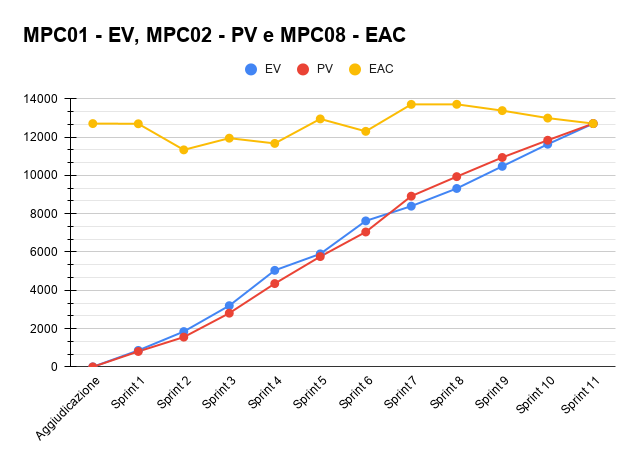
\includegraphics[scale=0.65]{../../../Assets/Grafici/EV_PV_EAC.png}}
            \caption{Grafico per sprint di MPC01, MPC02 e MPC08}
        \end{figure}

        \noindent \textbf{RTB:} \\
        Il valore dell'Earned Value (EV) coincide con quello del Planned Value (PV) nello sprint 1. Negli sprint successivi, l'EV risulta essere sempre superiore. In particolare, nello sprint 4, supera il PV di circa \euro700. Nello sprint 6, l’EV accumulato raggiunge \euro 7623, superiore al PV accumulato, che è di \euro 7045, segno di un avanzamento complessivamente in anticipo rispetto a quanto pianificato. 
        \\\\
        \noindent \textbf{PB:} \\
        Negli sprint dal 7 all’11 si osserva un'inversione rispetto alla fase precedente. A partire dallo sprint 7, l’EV risulta inferiore al PV: in questo punto l’EV accumulato è \euro8393, contro un PV di circa \euro8915, indicando un leggero ritardo rispetto al piano.
        Negli sprint successivi il divario persiste ma tende progressivamente a ridursi: nello sprint 9 si riduce a \euro463 e nello sprint 10 a \euro208.
        Nello sprint 11, infine, EV e PV coincidono nuovamente al valore di budget disponibile, segnalando un recupero completo del ritardo accumulato e la terminazione del progetto.

    }
    \newpage
    \subsection{MPC03, MPC08 e MPC09: Actual Cost, Estimate At Completion e Estimate To Complete}{
        \begin{figure}[H]
            \centering
            \fbox{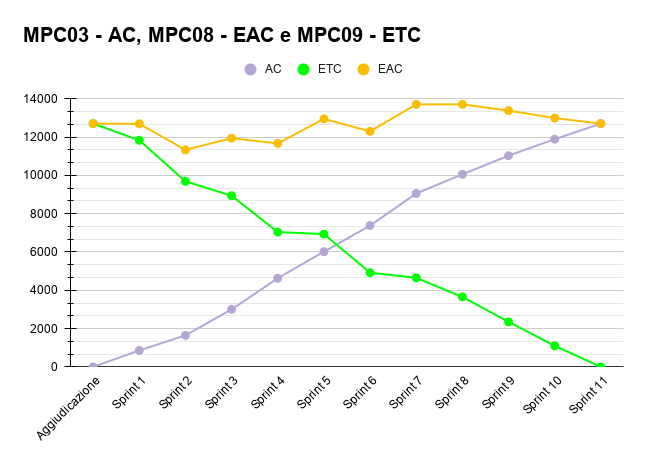
\includegraphics[scale=0.65]{../../../Assets/Grafici/AC_EAC_ETC.png}}
            \caption{Grafico per sprint di MPC03, MPC08 e MPC09}
        \end{figure}

        \noindent \textbf{RTB:} \\
        Il valore dell'Actual Cost (AC) cresce durante tutti gli sprint per raggiungere \euro7380 allo sprint 6. Il valore dell'Estimate To Complete (ETC) diminuisce circa della stessa quantità in quasi tutti gli sprint, e questo è indice di una regolare progressione nel progetto. Solo durante lo sprint 5, il valore dell'EAC si mantiene pressoché inalterato nonostante un incremento dell'AC di \euro1385. Durante il periodo 5 il team non ha fatto dei progressi sostanziali per terminare il lavoro necessario alla candidatura per la RTB, e li ha anzi relegati quasi totalmente allo sprint 6.
        \\\\
        \noindent \textbf{PB:} \\
        A partire dallo sprint 7, l’Actual Cost (AC) continua a crescere in modo regolare, passando da circa \euro9055 nello sprint 7 fino a \euro12700 nello sprint 11, indicando un avanzamento costante delle attività. Parallelamente, l’Estimate To Complete (ETC) diminuisce in maniera significativa e pressoché continua: da \euro4652 nello sprint 7 fino ad annullarsi nello sprint 11. L'andamento di questa metrica (e di quella speculare Estimate At Completion) riflette il progressivo completamento del lavoro residuo, senza evidenti rallentamenti nelle fasi finali.

    }
    \newpage
    \subsection{MPC04 e MPC05: Cost Variance e Schedule Variance}{
        \begin{figure}[H]
            \centering
            \fbox{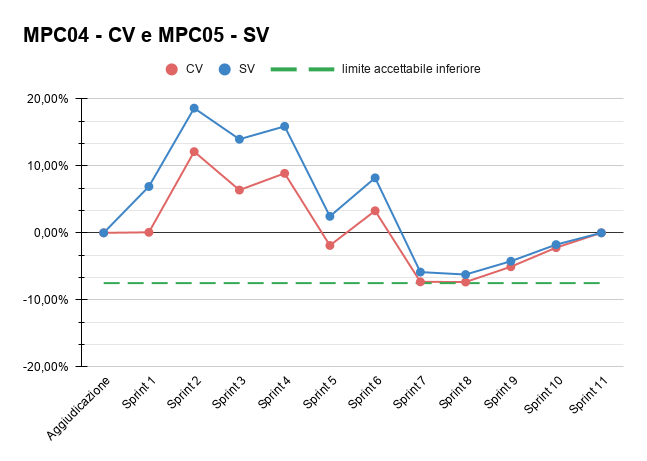
\includegraphics[scale=0.65]{../../../Assets/Grafici/CV_SV.png}}
            \caption{Grafico per sprint di MPC04 e MPC05}
        \end{figure}

        \noindent \textbf{RTB:} 
        \begin{itemize}[labelindent=0pt, leftmargin=*]
            \item Il Cost Variance (CV) assume valore positivo negli sprint 2, 3, 4 e 6, indicando che il progetto è in generale sotto budget. Durante lo sprint 2 il valore prodotto (l'EV) supera di oltre il 12\% l'ammontare dei costi (l'AC). Solo in corrispondenza dello sprint 5, il progetto va leggermente sopra budget. 
            \item Lo Schedule Variance (SV) assume sempre valore positivo (fino allo sprint 6). Di conseguenza, il progetto è in linea o avanti con i tempi. In particolare, durante lo sprint 2 è evidente come il valore prodotto (l'EV) superi quasi del 20\% quello pianificato (il PV). In questo periodo, infatti, il team ha avuto la possibilità di rendere le proprie ore molto produttive.
        \end{itemize}
        
        \noindent \\ \textbf{PB:}
        \begin{itemize}[labelindent=0pt, leftmargin=*]
            \item A partire dallo sprint 7, il Cost Variance (CV) assume valori negativi, indicando che il progetto entra in una fase sopra budget. In particolare, negli sprint 7 e 8 il CV si attesta intorno al -7\%, portandosi a ridosso della soglia di accettabilità. Negli sprint successivi si osserva però un progressivo recupero: il valore risale fino a circa -2\% nello sprint 10, per poi tornare a 0 nello sprint 11.
            \item Analogamente, lo Schedule Variance (SV) diventa negativo a partire dallo sprint 7, segnalando un ritardo rispetto alla pianificazione. Il valore minimo si registra tra gli sprint 7 e 8 (circa -6\%). Anche in questo caso si osserva un miglioramento graduale negli sprint successivi: il ritardo si riduce progressivamente fino ad annullarsi nello sprint 11, dove il progetto risulta nuovamente in linea con i tempi previsti.
        \end{itemize}
    }
    \newpage
    \subsection{MPC06 e MPC07: Cost Performance Index e Schedule Performance Index}{
        \begin{figure}[H]
            \centering
            \fbox{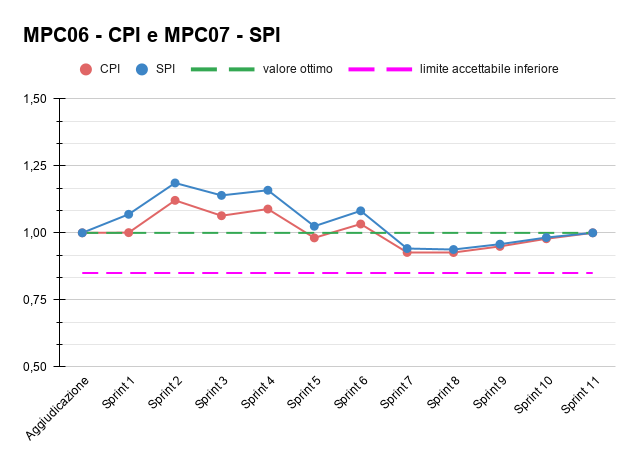
\includegraphics[scale=0.65]{../../../Assets/Grafici/CPI_SPI.png}}
            \caption{Grafico per sprint di MPC06 e MPC07}
        \end{figure}

        \noindent \textbf{RTB:}
        \begin{itemize}[labelindent=0pt, leftmargin=*]
            \item Il Cost Performance Index (CPI) assume valore ottimo nello sprint 1. Nei periodi 2, 3, 4 si alza complessivamente di 0,10. Torna a valori molto vicini a quello ottimo negli sprint 5, 6. Complessivamente, il rischio di superamento dei costi rimane basso.
            \item Lo Schedule Performance Index (SPI) assume valore quasi ottimo nello sprint 1, si alza nei tre sprint successivi fino a raggiungere il valore massimo di 1,18 nello sprint 2 e scende nuovamente attorno a 1 negli sprint 5 e 6. Il fatto che SPI non sia mai inferiore a 1 indica che il progetto non è mai in ritardo con i tempi.
        \end{itemize} 
        
        \noindent \\ \textbf{PB:}
        \begin{itemize}[labelindent=0pt, leftmargin=*]
            \item Dallo sprint 7, il Cost Performance Index (CPI) scende al di sotto del valore ottimo, assumendo valori inferiori a 1 (circa 0,93 negli sprint 7 e 8), indicando una fase in cui i costi superano il valore prodotto. Negli sprint successivi si osserva tuttavia un recupero progressivo: il CPI cresce gradualmente fino a riavvicinarsi al valore ottimo negli sprint 9 e 10, per poi attestarsi esattamente a 1 nello sprint 11.
            \item Lo Schedule Performance Index (SPI) scende sotto il valore ottimo a partire dallo sprint 7 (circa 0,94), evidenziando un ritardo rispetto alla pianificazione. Il valore rimane inferiore a 1 anche negli sprint 8 e 9. Nello sprint 10 lo SPI è ormai prossimo a 1 e nello sprint 11 raggiunge il valore ottimo.
        \end{itemize}
        
    }
    \newpage
    \subsection{MPC08: Estimate At Completion}{
        \begin{figure}[H]
            \centering
            \fbox{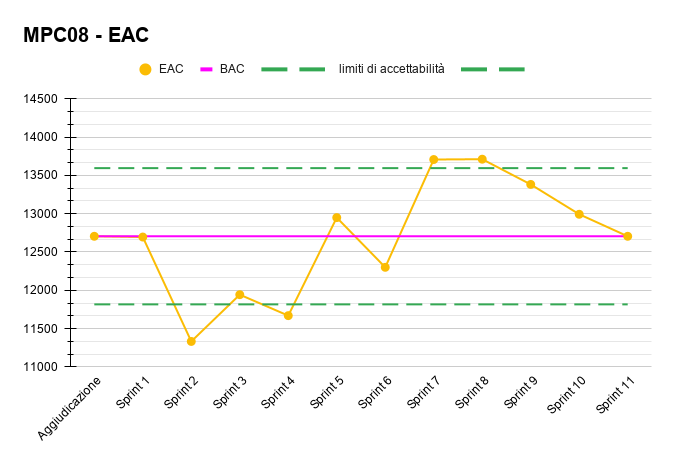
\includegraphics[scale=0.65]{../../../Assets/Grafici/BAC_EAC.png}}
            \caption{Grafico per sprint di MPC08}
        \end{figure}

        \noindent \textbf{RTB:} \\
        Nello sprint 1 l'Estimate At Completion (EAC) rimane pressoché invariato rispetto al Budget At Completion (BAC). Diminuisce invece fin sotto il limite accettabile inferiore durante gli sprint 2 e 4. Durante questo periodo il team ha dunque prodotto più di quanto pianificato. Il valore si alza poi oltre il budget in corrispondenza dello sprint 5, segno di rallentamenti. È positivo il fatto che l'EAC non superi mai il limite accettabile superiore.
        \\\\
        \noindent \textbf{PB:} \\
        Negli sprint 7 e 8, l’Estimate At Completion (EAC) supera il Budget At Completion (BAC) e raggiunge valori superiori al limite accettabile superiore (che è di quasi \euro13600), evidenziando una fase di maggiore criticità e possibili inefficienze nei costi. Negli sprint successivi si registra tuttavia un'inversione di tendenza: dallo sprint 9 l’EAC rientra sotto il limite superiore e continua a diminuire progressivamente negli sprint 10 e 11. Nello sprint 11, infine, l’EAC converge nuovamente verso il BAC (circa €12700), indicando la chiusura del progetto in linea con il budget previsto.

    }
    \newpage
    \subsection{MPC10: Requirements Stability Index}{
        \begin{figure}[H]
            \centering
            \fbox{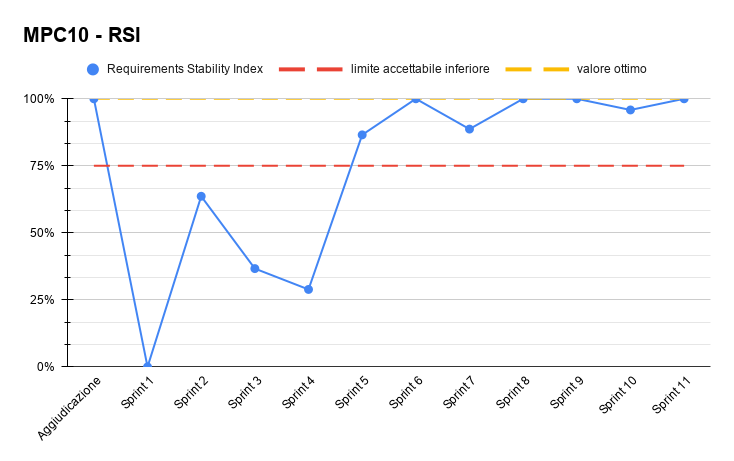
\includegraphics[scale=0.65]{../../../Assets/Grafici/RSI.png}}
            \caption{Grafico per sprint di MPC10}
        \end{figure}

        \noindent \textbf{RTB:} \\
        Il Requirements Stability Index (RSI) ha un picco negativo allo 0\% nello sprint 1 in quanto il team ha iniziato fin da subito a individuare i requisiti. Dopo un aumento in corrispondenza dello sprint 2, si registrano ulteriori flessioni negative al di sotto del limite inferiore di accettabilità in corrispondenza degli sprint 3 e 4 (37\% e 29\%). Durante questi periodi, infatti, il team ha effettuato colloqui aggiuntivi con l'azienda proponente per analizzare in profondità il capitolato d'appalto e ha di conseguenza aggiunto e modificato diversi requisiti. Il valore diventa infine accettabile a partire dallo sprint 5. 
        \\\\
        \noindent \textbf{PB:} \\
        Durante le attività di questa baseline si ha la stabilizzazione del RSI al di sopra della soglia inferiore di accettabilità. Nello sprint 7, il suo valore è di 89\% per via delle correzioni richieste dal prof. Cardin sull'Analisi dei Requisiti. Nei periodi 8 e 9 non si registrano cambiamenti e la metrica assume dunque valore ottimo. Nello sprint 10 il valore del RSI scende leggermente (a 96\%) a causa dell'adeguamento di alcuni requisiti agli scenari d'uso implementati nel progetto. Lo sprint 11 registra il ritorno della metrica al 100\%.
    }
    \newpage
    \subsection{MPC13: Indice di Gulpease}{
        \begin{figure}[H]
            \centering
            \fbox{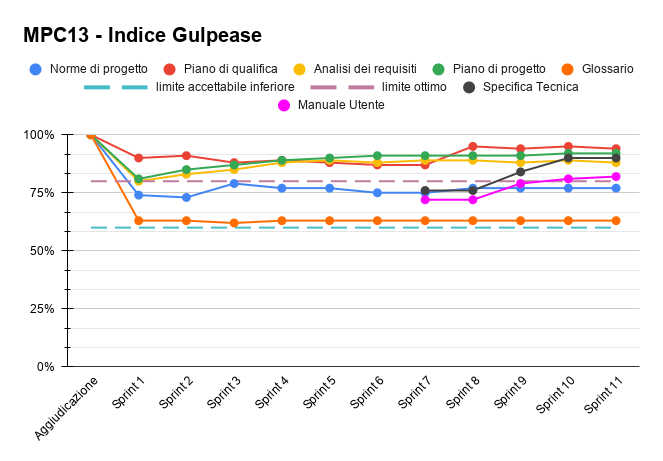
\includegraphics[scale=0.65]{../../../Assets/Grafici/Gulpease.png}}
            \caption{Grafico per sprint di MPC13}
        \end{figure}

        \noindent \textbf{RTB:} \\
        Il grafico mostra una chiara propensione del team alla cura della leggibilità dei documenti. L'indice di Gulpease si è infatti mantenuto al di sopra del valore di accettabilità per tutti i documenti durante tutti gli sprint.
        \begin{itemize}[labelindent=0pt, leftmargin=*]
            \item L'Analisi dei Requisiti ha un valore sempre ottimo e in crescita, che raggiunge il massimo (88\%) nello sprint 6.
            \item Simile è l'andamento dell'indice del Piano di Progetto, con il massimo (91\%) nello sprint 6.
            \item Il Piano di Qualifica ha un indice sempre ottimo ma che decresce a partire dallo sprint 2 (il cui valore è 91\%).
            \item Le Norme di Progetto hanno un valore di leggibilità accettabile che raggiunge il massimo nello sprint 2 (79\%) e che può dunque essere incrementato. 
            \item Il Glossario è il documento meno leggibile con un indice di Gulpease stabile al 63\%, legato alla presenza di termini tecnici e frasi brevi.
        \end{itemize}
        
        \noindent \\ \textbf{PB:} \\
        Il grafico conferma che, anche negli sprint dal 7 all’11, il team mantiene una forte attenzione alla leggibilità: l’indice di Gulpease resta sempre al di sopra del limite di accettabilità per tutti i documenti, con valori in alcuni casi superiori a quelli ottimali.
        \begin{itemize}[labelindent=0pt, leftmargin=*]
            \item L'Analisi dei Requisiti mantiene valori elevati e stabili dopo lo sprint 6; l'indice di Gulpease si stabilizza infatti sull'89\%.
            \item Il Piano di Progetto diventa via via più leggibile, fino a raggiungere il valore di 92\% negli sprint 10 e 11.
            \item Il Gulpease del Piano di Qualifica mostra una crescita significativa a partire dallo sprint 8 (momento in cui raggiunge il 95\%), per via delle correzioni apportate in seguito alla RTB.
            \item Le Norme di Progetto evidenziano invece una leggibilità stabile al 77\% (al di sotto del valore ottimo), nonostante le modifiche effettuate durante le attività di questa baseline.
            \item Il Glossario si mantiene stabile intorno al 63\%, confermandosi il documento meno leggibile a causa della natura tecnica dei contenuti.
            \item Il Manuale Utente, introdotto a partire dallo sprint 7, presenta valori inizialmente più bassi (72\%) ma in crescita costante fino a oltre l’80\% (limite per un indice ottimo) nello sprint 11.
            \item La Specifica Tecnica, che compare anch'essa nello sprint 7, parte dal 76\% ma migliora progressivamente la chiarezza espositiva fino ad arrivare al 90\%.
        \end{itemize}
    }
    \newpage
    \subsection{MPC14: Correttezza ortografica}{
        \begin{figure}[H]
            \centering
            \fbox{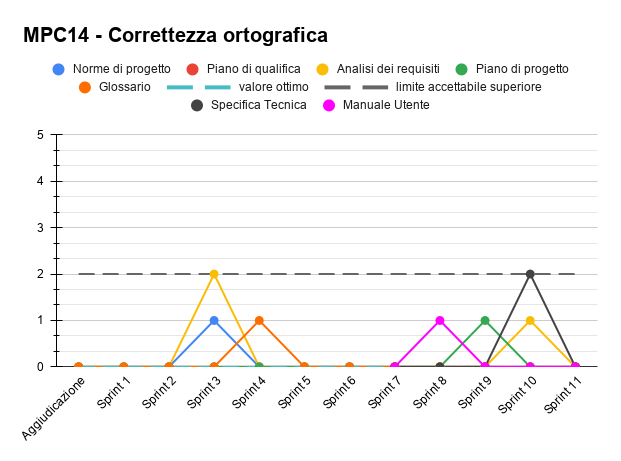
\includegraphics[scale=0.65]{../../../Assets/Grafici/Correttezza.png}}
            \caption{Grafico per sprint di MPC14}
        \end{figure}

        \noindent \textbf{RTB:} \\
        Al termine dei primi due sprint non sono stati rilevati errori ortografici. Al termine degli sprint 3 sono invece stati trovati 2 errori nell'Analisi dei Requisiti e 1 nelle Norme di Progetto. In questo periodo, tali documenti sono cresciuti molto in dimensione. Nello sprint 4, è stato segnalato un errore nel Glossario. Negli sprint 5 e 6, il team ha raggiunto il valore ottimo grazie a revisioni più attente.
        \\\\
        \noindent \textbf{PB:} \\
        Negli sprint dal 7 all’11, la correttezza ortografica rimane complessivamente elevata, con un numero di errori contenuto e sempre entro il limite accettabile. Nello sprint 7 non vengono rilevati errori, confermando il mantenimento del valore ottimo raggiunto negli sprint precedenti. Gli sprint 8 e 9 registrano un errore ciascuno, di cui quello nel Manuale Utente è dovuto alla recente introduzione del documento. Nello sprint 10 si rilevano due errori nella Specifica Tecnica e uno nell'Analisi dei Requisiti, rappresentando il punto di maggiore criticità del periodo, pur rimanendo entro i limiti accettabili. Nello sprint 11 il team recupera completamente, riportando tutti i documenti a zero errori e ristabilendo il valore ottimo grazie a un'attività di revisione finale accurata.

    }
    \newpage
    \subsection{MPC15: Code coverage}{
        \begin{figure}[H]
            \centering
            \fbox{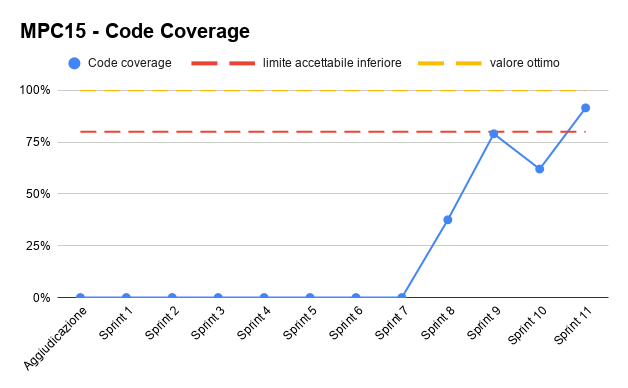
\includegraphics[scale=0.65]{../../../Assets/Grafici/CodeCoverage.png}}
            \caption{Grafico per sprint di MPC15}
        \end{figure}

        \noindent \textbf{RTB:} \\
        Misurazione non disponibile in questa baseline.
        \\\\
        \noindent \textbf{PB:} \\
        Il code coverage rimane nullo fino allo sprint 7 per via dell'assenza di test automatizzati nel processo di sviluppo del MVP. A partire dallo sprint 8 si osserva un primo incremento significativo (38\%). Nello sprint successivo la metrica cresce ancora e raggiunge il 79\%, appena sotto il limite accettabile (80\%). Lo sprint 10 registra tuttavia una flessione negativa (al 62\%), legata all'aggiunta di nuove funzionalità non ancora coperte da test. Infine, nello sprint 11 il coverage aumenta ulteriormente fino a 92\%, avvicinandosi al valore ottimo e indicando un consolidamento delle attività di testing e una buona copertura complessiva del codice del progetto.

    }
    \newpage
    \subsection{MPC16: Test Success Rate}{
        \begin{figure}[H]
            \centering
            \fbox{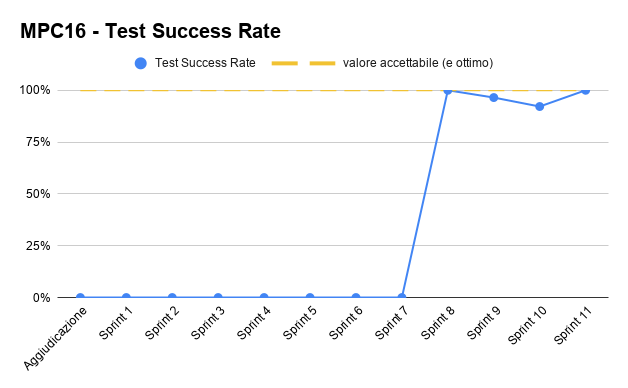
\includegraphics[scale=0.65]{../../../Assets/Grafici/TestSuccessRate.png}}
            \caption{Grafico per sprint di MPC16}
        \end{figure}

        \noindent \textbf{RTB:} \\
        Misurazione non disponibile in questa baseline.
        \\\\
        \noindent \textbf{PB:} \\
        Nello sprint 7, durante il quale sono stati aggiunti i primi test, il valore del Test Success Rate è massimo. 
    }
    \newpage
    \subsection{MPC17: Quality Metrics Satisfied}{
        \begin{figure}[H]
            \centering
            \fbox{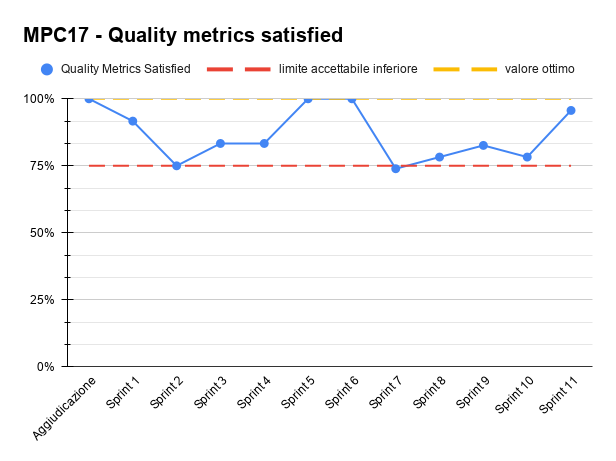
\includegraphics[scale=0.65]{../../../Assets/Grafici/QualityMetricsSatisfied.png}}
            \caption{Grafico per sprint di MPC17}
        \end{figure}

        \noindent \textbf{RTB:} \\
        Fin dal primo sprint, non tutte le metriche sono risultate soddisfatte. Durante gli sprint 2, 3 e 4, centrali per lo svolgimento dei compiti, il valore di Quality Metrics Satisfied è rimasto basso, ma comunque sopra la soglia di accettabilità (75\%). Il team giustifica questo con la poca esperienza dei membri nel gestire un tale progetto in modo efficiente. Durante gli sprint 5 e 6, in cui si è raggiunto il valore ottimo del 100\%, è evidente una presa di coscienza che ha portato alla risoluzione delle criticità.
        \\\\
        \noindent \textbf{PB:} \\
        //To Do
    }
    \newpage
    \subsection{MPC18: Non Calculated Risk}{
        \begin{figure}[H]
            \centering
            \fbox{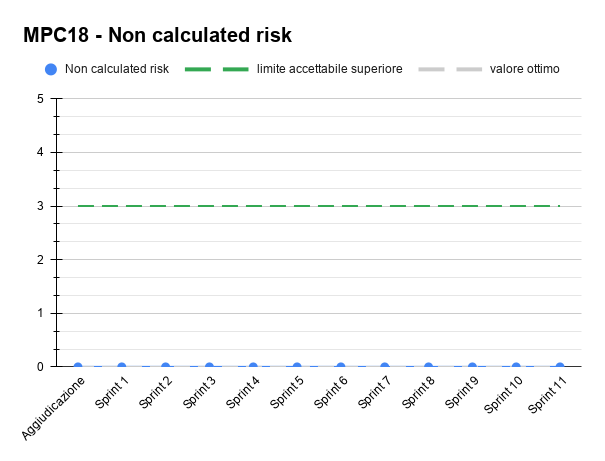
\includegraphics[scale=0.65]{../../../Assets/Grafici/NonCalculatedRisk.png}}
            \caption{Grafico per sprint di MPC18}
        \end{figure}

        \noindent \textbf{RTB:} \\
        Non si sono mai presentati rischi non attesi durante gli sprint. Ciò significa che il team è riuscito a individuare efficacemente e sapientemente i rischi all'inizio della RTB e prima di ogni nuovo sprint e che si è adoperato fin da subito per cercare di mitigarli.
        \\\\
        \noindent \textbf{PB:} \\
        //To Do
    }
    \newpage
    \subsection{MPD01: Requisiti obbligatori soddisfatti}{
        \begin{figure}[H]
            \centering
            \fbox{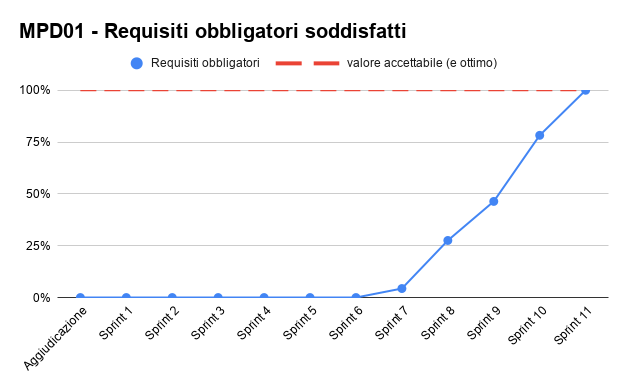
\includegraphics[scale=0.65]{../../../Assets/Grafici/RequisitiObbligatoriSoddisfatti.png}}
            \caption{Grafico per sprint di MPD01}
        \end{figure}

        \noindent \textbf{RTB:} \\
        Misurazione non disponibile in questa baseline.
        \\\\
        \noindent \textbf{PB:} \\
        //To Do
    }
    \newpage
    \subsection{MPD02 e MPD03: Requisiti desiderabili soddisfatti e Requisiti opzionali soddisfatti}{
        \begin{figure}[H]
            \centering
            \fbox{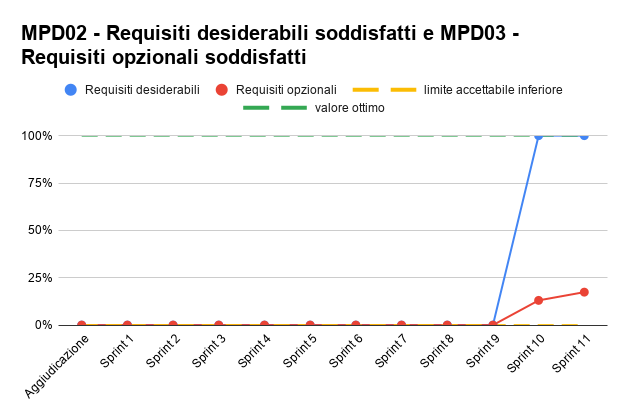
\includegraphics[scale=0.65]{../../../Assets/Grafici/RequisitiDesiderabiliOpzionaliSoddisfatti.png}}
            \caption{Grafico per sprint di MPD02 e MPD03}
        \end{figure}

        \noindent \textbf{RTB:} \\
        Misurazione non disponibile in questa baseline.
        \\\\
        \noindent \textbf{PB:} \\
        //To Do
    }
    \newpage
    \subsection{MPD04: Branch coverage}{
        \begin{figure}[H]
            \centering
            \fbox{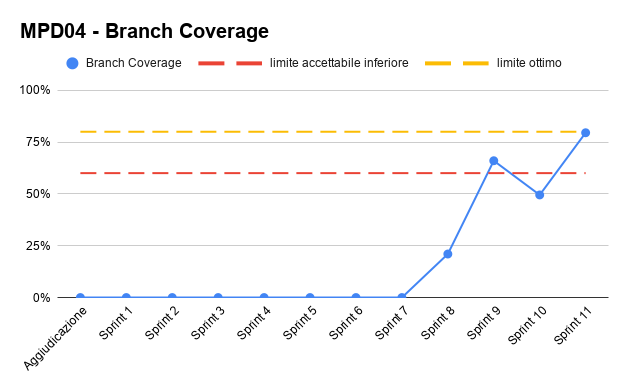
\includegraphics[scale=0.65]{../../../Assets/Grafici/BranchCoverage.png}}
            \caption{Grafico per sprint di MPD04}
        \end{figure}

        \noindent \textbf{RTB:} \\
        Misurazione non disponibile in questa baseline.
        \\\\
        \noindent \textbf{PB:} \\
        //To Do
    }
    \newpage
    \subsection{MPD05: Statement coverage}{
        \begin{figure}[H]
            \centering
            \fbox{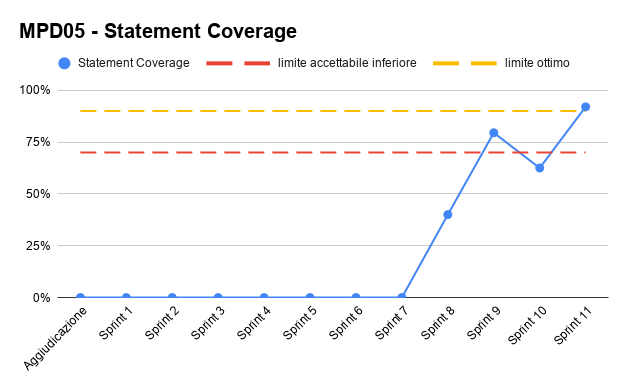
\includegraphics[scale=0.65]{../../../Assets/Grafici/StatementCoverage.png}}
            \caption{Grafico per sprint di MPD05}
        \end{figure}

        \noindent \textbf{RTB:} \\
        Misurazione non disponibile in questa baseline.
        \\\\
        \noindent \textbf{PB:} \\
        //To Do
    }
}

\end{document}

